\section{Method}
\subsection{Oscillator - 555 Timer IC}
\label{sec:555}
The first attempt made for the oscillators is to use a 555 timer chip to directly create an audible frequency square wave signal. The frequency of the 555 IC is determined by the size of the resistances, $R_1$ and $R_2$, and the capacitor, $C$, as located in figure~\ref{fig:555}.

\begin{figure}[htbp]
	\begin{center}
		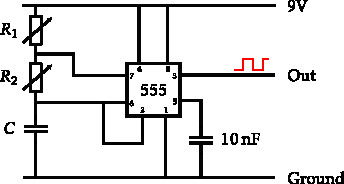
\includegraphics[scale=1.2]{report_img/555}
		\caption{Circuit diagram of the 555 timer IC with the immediate components used to make a VCO.}
		\label{fig:555}
	\end{center}
\end{figure}

The signal is generated by the chip using a series of capacitors and components contained within, a circuit diagram for the 555 can be seen in appendix~\ref{app:555}. The chip is connected in the astable mode so that the output signal is a continuous stream of rectangular pulses with a given frequency that obey equations (\ref{eqn:555freq}), (\ref{eqn:555high}) and (\ref{eqn:555low}), where $\tau_{\text{high}}$ is the time spent in the high voltage position and $\tau_{\text{low}}$ is the low time.\cite{NE555}
\begin{align}
	\label{eqn:555freq}
	f &= \frac{1}{\ln{2}C(R_1+R_2)}, \\
	\label{eqn:555high}
	\tau_{\text{high}} &= \ln{2}C(R_1+R_2), \\
	\label{eqn:555low}
	\tau_{\text{low}} &= \ln{2}CR_2. 
\end{align}
With two chips combined, a high degree of control over the output can be achieved by varying the value of the resistors. As a proof of concept, the circuit in figure \ref{fig:2x555} was built and a variable resistor in the form of an LDR was added. This allowed the pitch and volume to be controlled remotely using the fingers.

\begin{figure}[htbp]
	\begin{center}
		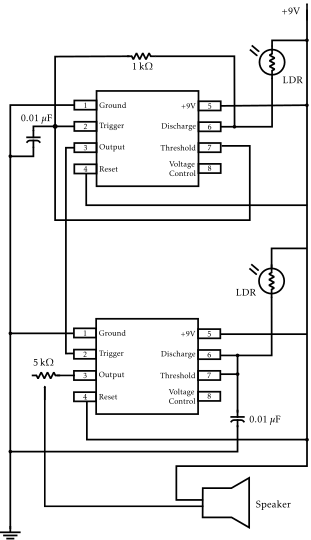
\includegraphics[scale=0.8,angle=90]{report_img/2x555}
		\caption{Circuit diagram of the two 555 timer ICs used to make a rudimentary resistance controlled theremin.}
		\label{fig:2x555}
	\end{center}
\end{figure}

\subsection{Oscillator - HEF4046 IC}
\label{sec:4046}
Though a controllable waveform in the audible frequency range was produced using the previously described 555 timer method, the sound was not pleasant as the wave was square shape and so does not resemble the ideal sinusoidal sound wave. In an attempt to improve the quality of this sound, an alternative VCO chip is tried. The first choice is the 8068 chip but this is no longer in commercial production, so a close relative, the 4046 chip, is used.

This chip contains several components that shall not be used, but importantly has a voltage controlled oscillator that can be used independently. The circuit diagram is shown in appendix~\ref{app:4046}. Pins 4, 6, 7, 10, 13, 15 and 16 are used with others left open.

Under these conditions, with a capacitance of 10\,nF and resistance of 10\,k$\Omega$, an audible sound was produced, shown, as measured on an oscilloscope, in figure~\ref{fig:4046square}.

\begin{figure}[htbp]
	\centering
		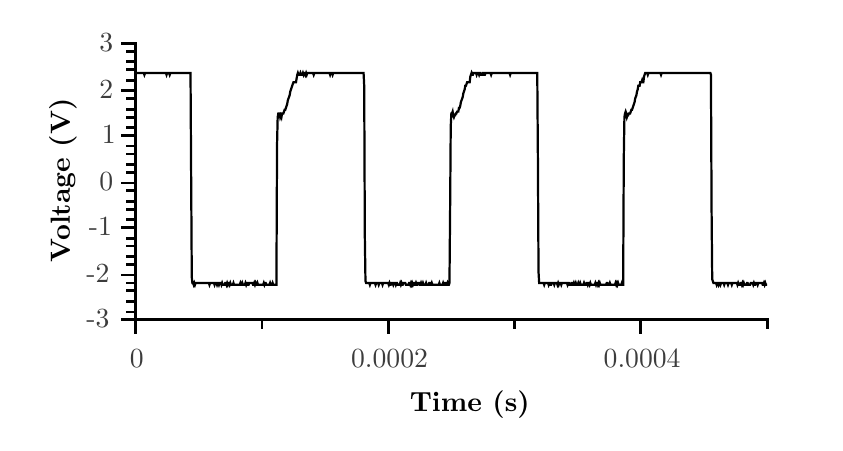
\begin{tikzpicture}{0pt}{0pt}{299pt}{150pt}
	\clip(0pt,150pt) -- (284.325pt,150pt) -- (284.325pt,7.36184pt) -- (0pt,7.36184pt) -- (0pt,150pt);
\begin{scope}
	\clip(38.9878pt,144.294pt) -- (267.209pt,144.294pt) -- (267.209pt,44.4478pt) -- (38.9878pt,44.4478pt) -- (38.9878pt,144.294pt);
	\color[gray]{0}
	\draw[line width=0.8pt, line join=miter, line cap=rect](39.216pt,133.644pt) -- (39.4442pt,133.644pt) -- (39.6724pt,133.644pt) -- (39.9006pt,133.644pt) -- (40.1289pt,133.644pt) -- (40.3571pt,133.644pt) -- (40.5853pt,133.644pt) -- (40.8135pt,133.644pt) -- (41.0418pt,133.644pt) -- (41.27pt,133.644pt) -- (41.4982pt,133.644pt) -- (41.7264pt,133.644pt) -- (41.9546pt,133.644pt) -- (42.1829pt,132.979pt) -- (42.4111pt,133.644pt) -- (42.6393pt,133.644pt) -- (42.8675pt,133.644pt) -- (43.0957pt,133.644pt) -- (43.324pt,133.644pt) -- (43.5522pt,133.644pt) -- (43.7804pt,133.644pt) -- (44.0086pt,133.644pt) -- (44.2368pt,133.644pt) -- (44.4651pt,133.644pt) -- (44.6933pt,133.644pt) -- (44.9215pt,133.644pt) -- (45.1497pt,133.644pt) -- (45.378pt,133.644pt) -- (45.6062pt,133.644pt) -- (45.8344pt,133.644pt) -- (46.0626pt,133.644pt) -- (46.2908pt,133.644pt) -- (46.5191pt,133.644pt) -- (46.7473pt,133.644pt) -- (46.9755pt,133.644pt) -- (47.2037pt,133.644pt) -- (47.4319pt,133.644pt) -- (47.6602pt,133.644pt) -- (47.8884pt,133.644pt) -- (48.1166pt,133.644pt) -- (48.3448pt,133.644pt) -- (48.573pt,133.644pt) -- (48.8013pt,133.644pt) -- (49.0295pt,133.644pt) -- (49.2577pt,133.644pt) -- (49.4859pt,133.644pt) -- (49.7142pt,133.644pt) -- (49.9424pt,133.644pt) -- (50.1706pt,132.979pt) -- (50.3988pt,133.644pt) -- (50.627pt,133.644pt) -- (50.8553pt,133.644pt) -- (51.0835pt,133.644pt) -- (51.3117pt,132.979pt) -- (51.5399pt,133.644pt) -- (51.7681pt,133.644pt) -- (51.9964pt,133.644pt) -- (52.2246pt,133.644pt) -- (52.4528pt,133.644pt) -- (52.681pt,133.644pt) -- (52.9092pt,133.644pt) -- (53.1375pt,133.644pt) -- (53.3657pt,133.644pt) -- (53.5939pt,133.644pt) -- (53.8221pt,133.644pt) -- (54.0504pt,133.644pt) -- (54.2786pt,133.644pt) -- (54.5068pt,133.644pt) -- (54.735pt,133.644pt) -- (54.9632pt,133.644pt) -- (55.1915pt,133.644pt) -- (55.4197pt,133.644pt) -- (55.6479pt,133.644pt) -- (55.8761pt,133.644pt) -- (56.1043pt,133.644pt) -- (56.3326pt,133.644pt) -- (56.5608pt,133.644pt) -- (56.789pt,133.644pt) -- (57.0172pt,133.644pt) -- (57.2454pt,133.644pt) -- (57.4737pt,133.644pt) -- (57.7019pt,133.644pt) -- (57.9301pt,133.644pt) -- (58.1583pt,133.644pt) -- (58.3866pt,133.644pt) -- (58.6148pt,133.644pt) -- (58.843pt,133.644pt) -- (59.0712pt,95.7024pt) -- (59.2994pt,59.7576pt) -- (59.5277pt,57.7607pt) -- (59.7559pt,57.7607pt) -- (59.9841pt,57.095pt) -- (60.2123pt,57.7607pt) -- (60.4405pt,57.095pt) -- (60.6688pt,57.7607pt) -- (60.897pt,57.7607pt) -- (61.1252pt,57.7607pt) -- (61.3534pt,57.7607pt) -- (61.5816pt,57.7607pt) -- (61.8099pt,57.7607pt) -- (62.0381pt,57.7607pt) -- (62.2663pt,57.7607pt) -- (62.4945pt,57.7607pt) -- (62.7228pt,57.7607pt) -- (62.951pt,57.7607pt) -- (63.1792pt,57.7607pt) -- (63.4074pt,57.7607pt) -- (63.6356pt,57.7607pt) -- (63.8639pt,57.7607pt) -- (64.0921pt,57.7607pt) -- (64.3203pt,57.7607pt) -- (64.5485pt,57.7607pt) -- (64.7767pt,57.7607pt) -- (65.005pt,57.7607pt) -- (65.2332pt,57.7607pt) -- (65.4614pt,57.7607pt) -- (65.6896pt,57.095pt) -- (65.9178pt,57.7607pt) -- (66.1461pt,57.7607pt) -- (66.3743pt,57.7607pt) -- (66.6025pt,57.7607pt) -- (66.8307pt,57.7607pt) -- (67.059pt,57.7607pt) -- (67.2872pt,57.7607pt) -- (67.5154pt,57.095pt) -- (67.7436pt,57.7607pt) -- (67.9718pt,57.7607pt) -- (68.2001pt,57.7607pt) -- (68.4283pt,57.095pt) -- (68.6565pt,57.7607pt) -- (68.8847pt,57.7607pt) -- (69.1129pt,57.095pt) -- (69.3412pt,57.7607pt) -- (69.5694pt,57.7607pt) -- (69.7976pt,57.7607pt) -- (70.0258pt,57.095pt) -- (70.254pt,57.7607pt) -- (70.4823pt,57.095pt) -- (70.7105pt,57.095pt) -- (70.9387pt,57.095pt) -- (71.1669pt,57.095pt) -- (71.3952pt,57.7607pt) -- (71.6234pt,57.7607pt) -- (71.8516pt,57.095pt) -- (72.0798pt,57.7607pt) -- (72.308pt,57.095pt) -- (72.5363pt,57.7607pt) -- (72.7645pt,57.7607pt) -- (72.9927pt,57.095pt) -- (73.2209pt,57.7607pt) -- (73.4491pt,57.095pt) -- (73.6774pt,57.095pt) -- (73.9056pt,57.095pt) -- (74.1338pt,57.095pt) -- (74.362pt,57.7607pt) -- (74.5902pt,57.095pt) -- (74.8185pt,57.095pt) -- (75.0467pt,57.095pt) -- (75.2749pt,57.095pt) -- (75.5031pt,57.095pt) -- (75.7314pt,57.095pt) -- (75.9596pt,57.095pt) -- (76.1878pt,57.095pt) -- (76.416pt,57.095pt) -- (76.6442pt,57.095pt) -- (76.8725pt,57.7607pt) -- (77.1007pt,57.095pt) -- (77.3289pt,57.095pt) -- (77.5571pt,57.7607pt) -- (77.7853pt,57.095pt) -- (78.0136pt,57.095pt) -- (78.2418pt,57.095pt) -- (78.47pt,57.095pt) -- (78.6982pt,57.7607pt) -- (78.9264pt,57.095pt) -- (79.1547pt,57.7607pt) -- (79.3829pt,57.7607pt) -- (79.6111pt,57.095pt) -- (79.8393pt,57.095pt) -- (80.0676pt,57.7607pt) -- (80.2958pt,57.7607pt) -- (80.524pt,57.7607pt) -- (80.7522pt,57.7607pt) -- (80.9804pt,57.7607pt) -- (81.2087pt,57.7607pt) -- (81.4369pt,57.095pt) -- (81.6651pt,57.095pt) -- (81.8933pt,57.7607pt) -- (82.1215pt,57.095pt) -- (82.3498pt,57.7607pt) -- (82.578pt,57.095pt) -- (82.8062pt,57.095pt) -- (83.0344pt,57.7607pt) -- (83.2626pt,57.095pt) -- (83.4909pt,57.095pt) -- (83.7191pt,57.095pt) -- (83.9473pt,57.095pt) -- (84.1755pt,57.095pt) -- (84.4038pt,57.095pt) -- (84.632pt,57.095pt) -- (84.8602pt,57.095pt) -- (85.0884pt,57.095pt) -- (85.3166pt,57.7607pt) -- (85.5449pt,57.095pt) -- (85.7731pt,57.7607pt) -- (86.0013pt,57.7607pt) -- (86.2295pt,57.095pt) -- (86.4577pt,57.095pt) -- (86.686pt,57.095pt) -- (86.9142pt,57.095pt) -- (87.1424pt,57.095pt) -- (87.3706pt,57.095pt) -- (87.5988pt,57.7607pt) -- (87.8271pt,57.095pt) -- (88.0553pt,57.095pt) -- (88.2835pt,57.095pt) -- (88.5117pt,57.7607pt) -- (88.74pt,57.095pt) -- (88.9682pt,57.095pt) -- (89.1964pt,57.095pt) -- (89.4246pt,57.095pt) -- (89.6528pt,57.095pt) -- (89.8811pt,57.095pt) -- (90.1093pt,107.684pt) -- (90.3375pt,117.669pt) -- (90.5657pt,119pt) -- (90.7939pt,119pt) -- (91.0222pt,119pt) -- (91.2504pt,117.669pt) -- (91.4786pt,118.334pt) -- (91.7068pt,117.669pt) -- (91.935pt,119pt) -- (92.1633pt,119pt) -- (92.3915pt,119pt) -- (92.6197pt,119.666pt) -- (92.8479pt,120.331pt) -- (93.0762pt,120.331pt) -- (93.3044pt,120.997pt) -- (93.5326pt,121.663pt) -- (93.7608pt,122.328pt) -- (93.989pt,123.659pt) -- (94.2173pt,124.325pt) -- (94.4455pt,124.991pt) -- (94.6737pt,125.656pt) -- (94.9019pt,126.988pt) -- (95.1301pt,127.653pt) -- (95.3584pt,128.319pt) -- (95.5866pt,128.985pt) -- (95.8148pt,129.65pt) -- (96.043pt,130.316pt) -- (96.2712pt,130.316pt) -- (96.4995pt,130.316pt) -- (96.7277pt,130.316pt) -- (96.9559pt,130.316pt) -- (97.1841pt,131.647pt) -- (97.4124pt,132.979pt) -- (97.6406pt,133.644pt) -- (97.8688pt,132.979pt) -- (98.097pt,132.979pt) -- (98.3252pt,132.979pt) -- (98.5535pt,133.644pt) -- (98.7817pt,132.979pt) -- (99.0099pt,132.979pt) -- (99.2381pt,132.979pt) -- (99.4663pt,133.644pt) -- (99.6946pt,132.979pt) -- (99.9228pt,133.644pt) -- (100.151pt,133.644pt) -- (100.379pt,132.979pt) -- (100.607pt,133.644pt) -- (100.836pt,132.979pt) -- (101.064pt,133.644pt) -- (101.292pt,133.644pt) -- (101.52pt,133.644pt) -- (101.749pt,133.644pt) -- (101.977pt,133.644pt) -- (102.205pt,133.644pt) -- (102.433pt,133.644pt) -- (102.661pt,133.644pt) -- (102.89pt,133.644pt) -- (103.118pt,133.644pt) -- (103.346pt,132.979pt) -- (103.574pt,133.644pt) -- (103.803pt,133.644pt) -- (104.031pt,133.644pt) -- (104.259pt,133.644pt) -- (104.487pt,133.644pt) -- (104.715pt,133.644pt) -- (104.944pt,133.644pt) -- (105.172pt,133.644pt) -- (105.4pt,133.644pt) -- (105.628pt,133.644pt) -- (105.857pt,133.644pt) -- (106.085pt,133.644pt) -- (106.313pt,133.644pt) -- (106.541pt,133.644pt) -- (106.769pt,133.644pt) -- (106.998pt,133.644pt) -- (107.226pt,133.644pt) -- (107.454pt,133.644pt) -- (107.682pt,133.644pt) -- (107.911pt,133.644pt) -- (108.139pt,133.644pt) -- (108.367pt,133.644pt) -- (108.595pt,133.644pt) -- (108.823pt,133.644pt) -- (109.052pt,133.644pt) -- (109.28pt,132.979pt) -- (109.508pt,133.644pt) -- (109.736pt,133.644pt) -- (109.965pt,133.644pt) -- (110.193pt,132.979pt) -- (110.421pt,133.644pt) -- (110.649pt,133.644pt) -- (110.877pt,133.644pt) -- (111.106pt,133.644pt) -- (111.334pt,133.644pt) -- (111.562pt,133.644pt) -- (111.79pt,133.644pt) -- (112.019pt,133.644pt) -- (112.247pt,133.644pt) -- (112.475pt,133.644pt) -- (112.703pt,133.644pt) -- (112.931pt,133.644pt) -- (113.16pt,133.644pt) -- (113.388pt,133.644pt) -- (113.616pt,133.644pt) -- (113.844pt,133.644pt) -- (114.072pt,133.644pt) -- (114.301pt,133.644pt) -- (114.529pt,133.644pt) -- (114.757pt,133.644pt) -- (114.985pt,133.644pt) -- (115.214pt,133.644pt) -- (115.442pt,133.644pt) -- (115.67pt,133.644pt) -- (115.898pt,133.644pt) -- (116.126pt,133.644pt) -- (116.355pt,133.644pt) -- (116.583pt,133.644pt) -- (116.811pt,133.644pt) -- (117.039pt,133.644pt) -- (117.268pt,133.644pt) -- (117.496pt,133.644pt) -- (117.724pt,133.644pt) -- (117.952pt,133.644pt) -- (118.18pt,133.644pt) -- (118.409pt,133.644pt) -- (118.637pt,133.644pt) -- (118.865pt,133.644pt) -- (119.093pt,133.644pt) -- (119.322pt,133.644pt) -- (119.55pt,133.644pt) -- (119.778pt,133.644pt) -- (120.006pt,133.644pt) -- (120.234pt,133.644pt) -- (120.463pt,133.644pt) -- (120.691pt,133.644pt) -- (120.919pt,133.644pt) -- (121.147pt,133.644pt) -- (121.376pt,133.644pt) -- (121.604pt,128.985pt) -- (121.832pt,74.4018pt) -- (122.06pt,58.4263pt) -- (122.288pt,57.7607pt) -- (122.517pt,57.7607pt) -- (122.745pt,57.7607pt) -- (122.973pt,57.7607pt) -- (123.201pt,57.7607pt) -- (123.43pt,57.7607pt) -- (123.658pt,57.095pt) -- (123.886pt,57.7607pt) -- (124.114pt,57.7607pt) -- (124.342pt,57.7607pt) -- (124.571pt,57.7607pt) -- (124.799pt,57.7607pt) -- (125.027pt,57.7607pt) -- (125.255pt,57.7607pt) -- (125.484pt,57.7607pt) -- (125.712pt,57.095pt) -- (125.94pt,57.7607pt) -- (126.168pt,57.7607pt) -- (126.396pt,57.7607pt) -- (126.625pt,57.7607pt) -- (126.853pt,57.095pt) -- (127.081pt,57.7607pt) -- (127.309pt,57.7607pt) -- (127.538pt,57.7607pt) -- (127.766pt,57.7607pt) -- (127.994pt,57.7607pt) -- (128.222pt,57.095pt) -- (128.45pt,57.7607pt) -- (128.679pt,57.7607pt) -- (128.907pt,57.7607pt) -- (129.135pt,57.7607pt) -- (129.363pt,57.7607pt) -- (129.592pt,57.7607pt) -- (129.82pt,57.7607pt) -- (130.048pt,57.7607pt) -- (130.276pt,57.7607pt) -- (130.504pt,57.095pt) -- (130.733pt,57.7607pt) -- (130.961pt,57.095pt) -- (131.189pt,57.095pt) -- (131.417pt,57.7607pt) -- (131.646pt,57.7607pt) -- (131.874pt,57.7607pt) -- (132.102pt,57.095pt) -- (132.33pt,57.7607pt) -- (132.558pt,57.7607pt) -- (132.787pt,57.7607pt) -- (133.015pt,57.095pt) -- (133.243pt,57.7607pt) -- (133.471pt,57.7607pt) -- (133.7pt,57.095pt) -- (133.928pt,57.095pt) -- (134.156pt,57.095pt) -- (134.384pt,57.095pt) -- (134.612pt,57.7607pt) -- (134.841pt,57.095pt) -- (135.069pt,57.7607pt) -- (135.297pt,57.095pt) -- (135.525pt,57.095pt) -- (135.753pt,57.7607pt) -- (135.982pt,57.7607pt) -- (136.21pt,57.7607pt) -- (136.438pt,57.7607pt) -- (136.666pt,57.095pt) -- (136.895pt,57.095pt) -- (137.123pt,57.095pt) -- (137.351pt,57.095pt) -- (137.579pt,57.095pt) -- (137.807pt,57.7607pt) -- (138.036pt,57.7607pt) -- (138.264pt,57.095pt) -- (138.492pt,57.7607pt) -- (138.72pt,57.095pt) -- (138.949pt,57.7607pt) -- (139.177pt,57.095pt) -- (139.405pt,57.7607pt) -- (139.633pt,57.7607pt) -- (139.861pt,57.095pt) -- (140.09pt,57.095pt) -- (140.318pt,57.7607pt) -- (140.546pt,57.095pt) -- (140.774pt,57.095pt) -- (141.003pt,57.7607pt) -- (141.231pt,57.7607pt) -- (141.459pt,57.7607pt) -- (141.687pt,57.095pt) -- (141.915pt,57.095pt) -- (142.144pt,57.7607pt) -- (142.372pt,57.095pt) -- (142.6pt,57.095pt) -- (142.828pt,57.7607pt) -- (143.057pt,57.095pt) -- (143.285pt,57.095pt) -- (143.513pt,57.095pt) -- (143.741pt,57.095pt) -- (143.969pt,57.7607pt) -- (144.198pt,57.095pt) -- (144.426pt,57.095pt) -- (144.654pt,57.095pt) -- (144.882pt,57.095pt) -- (145.111pt,57.7607pt) -- (145.339pt,57.7607pt) -- (145.567pt,57.095pt) -- (145.795pt,57.095pt) -- (146.023pt,57.7607pt) -- (146.252pt,57.095pt) -- (146.48pt,57.095pt) -- (146.708pt,57.095pt) -- (146.936pt,57.095pt) -- (147.165pt,57.095pt) -- (147.393pt,57.095pt) -- (147.621pt,57.095pt) -- (147.849pt,57.095pt) -- (148.077pt,57.095pt) -- (148.306pt,57.095pt) -- (148.534pt,57.095pt) -- (148.762pt,57.7607pt) -- (148.99pt,57.095pt) -- (149.219pt,57.095pt) -- (149.447pt,57.095pt) -- (149.675pt,57.095pt) -- (149.903pt,57.095pt) -- (150.131pt,57.7607pt) -- (150.36pt,57.095pt) -- (150.588pt,57.095pt) -- (150.816pt,57.7607pt) -- (151.044pt,57.7607pt) -- (151.273pt,57.095pt) -- (151.501pt,57.095pt) -- (151.729pt,57.7607pt) -- (151.957pt,57.095pt) -- (152.185pt,57.095pt) -- (152.414pt,57.7607pt) -- (152.642pt,83.7208pt) -- (152.87pt,114.34pt) -- (153.098pt,119pt) -- (153.327pt,119pt) -- (153.555pt,119.666pt) -- (153.783pt,118.334pt) -- (154.011pt,117.669pt) -- (154.239pt,118.334pt) -- (154.468pt,118.334pt) -- (154.696pt,119pt) -- (154.924pt,119pt) -- (155.152pt,119.666pt) -- (155.38pt,119.666pt) -- (155.609pt,119.666pt) -- (155.837pt,120.997pt) -- (156.065pt,120.997pt) -- (156.293pt,121.663pt) -- (156.522pt,122.994pt) -- (156.75pt,123.659pt) -- (156.978pt,124.325pt) -- (157.206pt,124.991pt) -- (157.434pt,126.322pt) -- (157.663pt,126.988pt) -- (157.891pt,127.653pt) -- (158.119pt,128.985pt) -- (158.347pt,128.985pt) -- (158.576pt,129.65pt) -- (158.804pt,130.316pt) -- (159.032pt,130.316pt) -- (159.26pt,130.316pt) -- (159.488pt,130.316pt) -- (159.717pt,130.316pt) -- (159.945pt,132.313pt) -- (160.173pt,132.979pt) -- (160.401pt,133.644pt) -- (160.63pt,132.979pt) -- (160.858pt,132.979pt) -- (161.086pt,133.644pt) -- (161.314pt,133.644pt) -- (161.542pt,133.644pt) -- (161.771pt,133.644pt) -- (161.999pt,133.644pt) -- (162.227pt,132.979pt) -- (162.455pt,133.644pt) -- (162.684pt,133.644pt) -- (162.912pt,133.644pt) -- (163.14pt,132.979pt) -- (163.368pt,133.644pt) -- (163.596pt,133.644pt) -- (163.825pt,132.979pt) -- (164.053pt,132.979pt) -- (164.281pt,132.979pt) -- (164.509pt,133.644pt) -- (164.738pt,133.644pt) -- (164.966pt,132.979pt) -- (165.194pt,132.979pt) -- (165.422pt,133.644pt) -- (165.65pt,133.644pt) -- (165.879pt,133.644pt) -- (166.107pt,133.644pt) -- (166.335pt,133.644pt) -- (166.563pt,133.644pt) -- (166.792pt,133.644pt) -- (167.02pt,133.644pt) -- (167.248pt,133.644pt) -- (167.476pt,132.979pt) -- (167.704pt,133.644pt) -- (167.933pt,133.644pt) -- (168.161pt,133.644pt) -- (168.389pt,133.644pt) -- (168.617pt,133.644pt) -- (168.846pt,133.644pt) -- (169.074pt,133.644pt) -- (169.302pt,133.644pt) -- (169.53pt,133.644pt) -- (169.758pt,133.644pt) -- (169.987pt,133.644pt) -- (170.215pt,133.644pt) -- (170.443pt,133.644pt) -- (170.671pt,133.644pt) -- (170.9pt,133.644pt) -- (171.128pt,133.644pt) -- (171.356pt,133.644pt) -- (171.584pt,133.644pt) -- (171.812pt,133.644pt) -- (172.041pt,133.644pt) -- (172.269pt,133.644pt) -- (172.497pt,133.644pt) -- (172.725pt,133.644pt) -- (172.954pt,133.644pt) -- (173.182pt,133.644pt) -- (173.41pt,133.644pt) -- (173.638pt,133.644pt) -- (173.866pt,133.644pt) -- (174.095pt,133.644pt) -- (174.323pt,132.979pt) -- (174.551pt,133.644pt) -- (174.779pt,133.644pt) -- (175.008pt,133.644pt) -- (175.236pt,133.644pt) -- (175.464pt,133.644pt) -- (175.692pt,133.644pt) -- (175.92pt,133.644pt) -- (176.149pt,133.644pt) -- (176.377pt,133.644pt) -- (176.605pt,133.644pt) -- (176.833pt,133.644pt) -- (177.061pt,133.644pt) -- (177.29pt,133.644pt) -- (177.518pt,133.644pt) -- (177.746pt,133.644pt) -- (177.974pt,133.644pt) -- (178.203pt,133.644pt) -- (178.431pt,133.644pt) -- (178.659pt,133.644pt) -- (178.887pt,133.644pt) -- (179.115pt,133.644pt) -- (179.344pt,133.644pt) -- (179.572pt,133.644pt) -- (179.8pt,133.644pt) -- (180.028pt,133.644pt) -- (180.257pt,133.644pt) -- (180.485pt,133.644pt) -- (180.713pt,133.644pt) -- (180.941pt,133.644pt) -- (181.169pt,133.644pt) -- (181.398pt,133.644pt) -- (181.626pt,133.644pt) -- (181.854pt,133.644pt) -- (182.082pt,133.644pt) -- (182.311pt,133.644pt) -- (182.539pt,133.644pt) -- (182.767pt,133.644pt) -- (182.995pt,133.644pt) -- (183.223pt,133.644pt) -- (183.452pt,133.644pt) -- (183.68pt,133.644pt) -- (183.908pt,133.644pt) -- (184.136pt,133.644pt) -- (184.365pt,103.025pt) -- (184.593pt,61.7545pt) -- (184.821pt,57.7607pt) -- (185.049pt,57.7607pt) -- (185.277pt,57.7607pt) -- (185.506pt,57.7607pt) -- (185.734pt,57.7607pt) -- (185.962pt,57.7607pt) -- (186.19pt,57.7607pt) -- (186.419pt,57.7607pt) -- (186.647pt,57.095pt) -- (186.875pt,57.7607pt) -- (187.103pt,57.7607pt) -- (187.331pt,57.7607pt) -- (187.56pt,57.7607pt) -- (187.788pt,57.7607pt) -- (188.016pt,57.7607pt) -- (188.244pt,57.095pt) -- (188.473pt,57.7607pt) -- (188.701pt,57.7607pt) -- (188.929pt,57.095pt) -- (189.157pt,57.095pt) -- (189.385pt,57.7607pt) -- (189.614pt,57.7607pt) -- (189.842pt,57.7607pt) -- (190.07pt,57.7607pt) -- (190.298pt,57.095pt) -- (190.527pt,57.7607pt) -- (190.755pt,57.7607pt) -- (190.983pt,57.7607pt) -- (191.211pt,57.7607pt) -- (191.439pt,57.095pt) -- (191.668pt,57.7607pt) -- (191.896pt,57.095pt) -- (192.124pt,57.7607pt) -- (192.352pt,57.7607pt) -- (192.581pt,57.7607pt) -- (192.809pt,57.095pt) -- (193.037pt,57.7607pt) -- (193.265pt,57.7607pt) -- (193.493pt,57.7607pt) -- (193.722pt,57.7607pt) -- (193.95pt,57.7607pt) -- (194.178pt,57.7607pt) -- (194.406pt,57.7607pt) -- (194.635pt,57.7607pt) -- (194.863pt,57.7607pt) -- (195.091pt,57.095pt) -- (195.319pt,57.7607pt) -- (195.547pt,57.7607pt) -- (195.776pt,57.095pt) -- (196.004pt,57.095pt) -- (196.232pt,57.095pt) -- (196.46pt,57.7607pt) -- (196.689pt,57.7607pt) -- (196.917pt,57.095pt) -- (197.145pt,57.095pt) -- (197.373pt,57.7607pt) -- (197.601pt,57.095pt) -- (197.83pt,57.095pt) -- (198.058pt,57.7607pt) -- (198.286pt,57.095pt) -- (198.514pt,57.095pt) -- (198.742pt,57.095pt) -- (198.971pt,57.7607pt) -- (199.199pt,57.095pt) -- (199.427pt,57.095pt) -- (199.655pt,57.7607pt) -- (199.884pt,57.095pt) -- (200.112pt,57.095pt) -- (200.34pt,57.095pt) -- (200.568pt,57.095pt) -- (200.796pt,57.095pt) -- (201.025pt,57.7607pt) -- (201.253pt,57.095pt) -- (201.481pt,57.095pt) -- (201.709pt,57.095pt) -- (201.938pt,57.7607pt) -- (202.166pt,57.7607pt) -- (202.394pt,57.095pt) -- (202.622pt,57.7607pt) -- (202.85pt,57.7607pt) -- (203.079pt,57.095pt) -- (203.307pt,57.7607pt) -- (203.535pt,57.095pt) -- (203.763pt,57.095pt) -- (203.992pt,57.095pt) -- (204.22pt,57.095pt) -- (204.448pt,57.095pt) -- (204.676pt,57.095pt) -- (204.904pt,57.095pt) -- (205.133pt,57.7607pt) -- (205.361pt,57.095pt) -- (205.589pt,57.7607pt) -- (205.817pt,57.7607pt) -- (206.046pt,57.095pt) -- (206.274pt,57.7607pt) -- (206.502pt,57.095pt) -- (206.73pt,57.7607pt) -- (206.958pt,57.095pt) -- (207.187pt,57.095pt) -- (207.415pt,57.095pt) -- (207.643pt,57.095pt) -- (207.871pt,57.095pt) -- (208.1pt,57.095pt) -- (208.328pt,57.095pt) -- (208.556pt,57.095pt) -- (208.784pt,57.095pt) -- (209.012pt,57.095pt) -- (209.241pt,57.7607pt) -- (209.469pt,57.7607pt) -- (209.697pt,57.095pt) -- (209.925pt,57.095pt) -- (210.154pt,57.095pt) -- (210.382pt,57.7607pt) -- (210.61pt,57.095pt) -- (210.838pt,57.095pt) -- (211.066pt,57.095pt) -- (211.295pt,57.095pt) -- (211.523pt,57.095pt) -- (211.751pt,57.095pt) -- (211.979pt,57.095pt) -- (212.208pt,57.095pt) -- (212.436pt,57.7607pt) -- (212.664pt,57.095pt) -- (212.892pt,57.7607pt) -- (213.12pt,57.095pt) -- (213.349pt,57.7607pt) -- (213.577pt,57.095pt) -- (213.805pt,57.095pt) -- (214.033pt,57.095pt) -- (214.262pt,57.095pt) -- (214.49pt,57.095pt) -- (214.718pt,57.7607pt) -- (214.946pt,57.095pt) -- (215.174pt,57.095pt) -- (215.403pt,103.025pt) -- (215.631pt,117.669pt) -- (215.859pt,119pt) -- (216.087pt,119.666pt) -- (216.316pt,119pt) -- (216.544pt,117.669pt) -- (216.772pt,118.334pt) -- (217pt,118.334pt) -- (217.228pt,119pt) -- (217.457pt,119pt) -- (217.685pt,119pt) -- (217.913pt,119.666pt) -- (218.141pt,120.331pt) -- (218.37pt,120.331pt) -- (218.598pt,120.997pt) -- (218.826pt,121.663pt) -- (219.054pt,122.328pt) -- (219.282pt,122.994pt) -- (219.511pt,124.325pt) -- (219.739pt,124.991pt) -- (219.967pt,125.656pt) -- (220.195pt,126.988pt) -- (220.423pt,127.653pt) -- (220.652pt,128.985pt) -- (220.88pt,128.985pt) -- (221.108pt,128.985pt) -- (221.336pt,130.316pt) -- (221.565pt,130.316pt) -- (221.793pt,130.316pt) -- (222.021pt,130.982pt) -- (222.249pt,130.316pt) -- (222.477pt,130.316pt) -- (222.706pt,132.313pt) -- (222.934pt,132.979pt) -- (223.162pt,133.644pt) -- (223.39pt,133.644pt) -- (223.619pt,133.644pt) -- (223.847pt,133.644pt) -- (224.075pt,132.979pt) -- (224.303pt,133.644pt) -- (224.531pt,133.644pt) -- (224.76pt,133.644pt) -- (224.988pt,133.644pt) -- (225.216pt,133.644pt) -- (225.444pt,133.644pt) -- (225.673pt,133.644pt) -- (225.901pt,133.644pt) -- (226.129pt,133.644pt) -- (226.357pt,133.644pt) -- (226.585pt,133.644pt) -- (226.814pt,133.644pt) -- (227.042pt,133.644pt) -- (227.27pt,133.644pt) -- (227.498pt,133.644pt) -- (227.727pt,133.644pt) -- (227.955pt,133.644pt) -- (228.183pt,133.644pt) -- (228.411pt,133.644pt) -- (228.639pt,133.644pt) -- (228.868pt,132.979pt) -- (229.096pt,133.644pt) -- (229.324pt,133.644pt) -- (229.552pt,133.644pt) -- (229.781pt,133.644pt) -- (230.009pt,133.644pt) -- (230.237pt,133.644pt) -- (230.465pt,133.644pt) -- (230.693pt,133.644pt) -- (230.922pt,133.644pt) -- (231.15pt,133.644pt) -- (231.378pt,133.644pt) -- (231.606pt,133.644pt) -- (231.835pt,133.644pt) -- (232.063pt,133.644pt) -- (232.291pt,133.644pt) -- (232.519pt,133.644pt) -- (232.747pt,133.644pt) -- (232.976pt,133.644pt) -- (233.204pt,133.644pt) -- (233.432pt,133.644pt) -- (233.66pt,133.644pt) -- (233.889pt,133.644pt) -- (234.117pt,133.644pt) -- (234.345pt,133.644pt) -- (234.573pt,133.644pt) -- (234.801pt,133.644pt) -- (235.03pt,133.644pt) -- (235.258pt,133.644pt) -- (235.486pt,133.644pt) -- (235.714pt,133.644pt) -- (235.943pt,133.644pt) -- (236.171pt,133.644pt) -- (236.399pt,133.644pt) -- (236.627pt,133.644pt) -- (236.855pt,133.644pt) -- (237.084pt,133.644pt) -- (237.312pt,133.644pt) -- (237.54pt,133.644pt) -- (237.768pt,133.644pt) -- (237.997pt,133.644pt) -- (238.225pt,133.644pt) -- (238.453pt,133.644pt) -- (238.681pt,133.644pt) -- (238.909pt,133.644pt) -- (239.138pt,133.644pt) -- (239.366pt,133.644pt) -- (239.594pt,133.644pt) -- (239.822pt,133.644pt) -- (240.051pt,133.644pt) -- (240.279pt,133.644pt) -- (240.507pt,133.644pt) -- (240.735pt,133.644pt) -- (240.963pt,133.644pt) -- (241.192pt,133.644pt) -- (241.42pt,133.644pt) -- (241.648pt,133.644pt) -- (241.876pt,133.644pt) -- (242.104pt,133.644pt) -- (242.333pt,133.644pt) -- (242.561pt,133.644pt) -- (242.789pt,133.644pt) -- (243.017pt,133.644pt) -- (243.246pt,133.644pt) -- (243.474pt,133.644pt) -- (243.702pt,133.644pt) -- (243.93pt,133.644pt) -- (244.158pt,133.644pt) -- (244.387pt,133.644pt) -- (244.615pt,133.644pt) -- (244.843pt,133.644pt) -- (245.071pt,133.644pt) -- (245.3pt,133.644pt) -- (245.528pt,133.644pt) -- (245.756pt,133.644pt) -- (245.984pt,133.644pt) -- (246.212pt,133.644pt) -- (246.441pt,133.644pt) -- (246.669pt,133.644pt) -- (246.897pt,132.979pt) -- (247.125pt,84.3864pt) -- (247.354pt,59.0919pt) -- (247.582pt,58.4263pt) -- (247.81pt,57.7607pt) -- (248.038pt,57.7607pt) -- (248.266pt,57.7607pt) -- (248.495pt,57.7607pt) -- (248.723pt,57.7607pt) -- (248.951pt,57.095pt) -- (249.179pt,57.7607pt) -- (249.408pt,57.7607pt) -- (249.636pt,57.095pt) -- (249.864pt,57.7607pt) -- (250.092pt,57.7607pt) -- (250.32pt,57.095pt) -- (250.549pt,57.7607pt) -- (250.777pt,57.7607pt) -- (251.005pt,57.7607pt) -- (251.233pt,57.7607pt) -- (251.462pt,57.7607pt) -- (251.69pt,57.095pt) -- (251.918pt,57.7607pt) -- (252.146pt,57.7607pt) -- (252.374pt,57.7607pt) -- (252.603pt,57.7607pt) -- (252.831pt,57.7607pt) -- (253.059pt,57.095pt) -- (253.287pt,57.7607pt) -- (253.516pt,57.7607pt) -- (253.744pt,57.7607pt) -- (253.972pt,57.7607pt) -- (254.2pt,57.7607pt) -- (254.428pt,57.095pt) -- (254.657pt,57.7607pt) -- (254.885pt,57.7607pt) -- (255.113pt,57.7607pt) -- (255.341pt,57.7607pt) -- (255.57pt,57.7607pt) -- (255.798pt,57.7607pt) -- (256.026pt,57.7607pt) -- (256.254pt,57.7607pt) -- (256.482pt,57.095pt) -- (256.711pt,57.7607pt) -- (256.939pt,57.095pt) -- (257.167pt,57.095pt) -- (257.395pt,57.095pt) -- (257.624pt,57.7607pt) -- (257.852pt,57.7607pt) -- (258.08pt,57.095pt) -- (258.308pt,57.7607pt) -- (258.536pt,57.095pt) -- (258.765pt,57.7607pt) -- (258.993pt,57.095pt) -- (259.221pt,57.095pt) -- (259.449pt,57.095pt) -- (259.678pt,57.095pt) -- (259.906pt,57.7607pt) -- (260.134pt,57.7607pt) -- (260.362pt,57.095pt) -- (260.59pt,57.095pt) -- (260.819pt,57.095pt) -- (261.047pt,57.095pt) -- (261.275pt,57.7607pt) -- (261.503pt,57.7607pt) -- (261.732pt,57.7607pt) -- (261.96pt,57.7607pt) -- (262.188pt,57.095pt) -- (262.416pt,57.7607pt) -- (262.644pt,57.095pt) -- (262.873pt,57.095pt) -- (263.101pt,57.7607pt) -- (263.329pt,57.7607pt) -- (263.557pt,57.7607pt) -- (263.785pt,57.095pt) -- (264.014pt,57.7607pt) -- (264.242pt,57.7607pt) -- (264.47pt,57.7607pt) -- (264.698pt,57.7607pt) -- (264.927pt,57.7607pt) -- (265.155pt,57.7607pt) -- (265.383pt,57.7607pt) -- (265.611pt,57.095pt) -- (265.839pt,57.095pt) -- (266.068pt,57.7607pt) -- (266.296pt,57.095pt) -- (266.524pt,57.7607pt) -- (266.752pt,57.095pt) -- (266.981pt,57.095pt) -- (267.209pt,57.095pt);
\end{scope}
\begin{scope}
	\color[gray]{0}
	\pgftext[center, base, at={\pgfpoint{15.2147pt}{94.8391pt}},rotate=90]{\textbf{Voltage (V)}}
	\color[gray]{0.235294}
	\pgftext[center, base, at={\pgfpoint{25.3628pt}{41.595pt}}]{-3}
	\pgftext[center, base, at={\pgfpoint{25.3628pt}{57.7607pt}}]{-2}
	\pgftext[center, base, at={\pgfpoint{26.3138pt}{74.8772pt}}]{-1}
	\pgftext[center, base, at={\pgfpoint{28.3716pt}{91.0429pt}}]{0}
	\pgftext[center, base, at={\pgfpoint{29.3225pt}{108.159pt}}]{1}
	\pgftext[center, base, at={\pgfpoint{28.3716pt}{124.325pt}}]{2}
	\pgftext[center, base, at={\pgfpoint{28.3716pt}{141.442pt}}]{3}
	\color[gray]{0}
	\draw[line width=1pt, line join=bevel, line cap=rect](38.9878pt,47.3005pt) -- (36.135pt,47.3005pt);
	\draw[line width=1pt, line join=bevel, line cap=rect](38.9878pt,51.1042pt) -- (36.135pt,51.1042pt);
	\draw[line width=1pt, line join=bevel, line cap=rect](38.9878pt,54.9079pt) -- (36.135pt,54.9079pt);
	\draw[line width=1pt, line join=bevel, line cap=rect](38.9878pt,57.7607pt) -- (36.135pt,57.7607pt);
	\draw[line width=1pt, line join=bevel, line cap=rect](38.9878pt,64.4171pt) -- (36.135pt,64.4171pt);
	\draw[line width=1pt, line join=bevel, line cap=rect](38.9878pt,67.2699pt) -- (36.135pt,67.2699pt);
	\draw[line width=1pt, line join=bevel, line cap=rect](38.9878pt,71.0736pt) -- (36.135pt,71.0736pt);
	\draw[line width=1pt, line join=bevel, line cap=rect](38.9878pt,73.9263pt) -- (36.135pt,73.9263pt);
	\draw[line width=1pt, line join=bevel, line cap=rect](38.9878pt,80.5828pt) -- (36.135pt,80.5828pt);
	\draw[line width=1pt, line join=bevel, line cap=rect](38.9878pt,84.3864pt) -- (36.135pt,84.3864pt);
	\draw[line width=1pt, line join=bevel, line cap=rect](38.9878pt,87.2392pt) -- (36.135pt,87.2392pt);
	\draw[line width=1pt, line join=bevel, line cap=rect](38.9878pt,91.0429pt) -- (36.135pt,91.0429pt);
	\draw[line width=1pt, line join=bevel, line cap=rect](38.9878pt,97.6993pt) -- (36.135pt,97.6993pt);
	\draw[line width=1pt, line join=bevel, line cap=rect](38.9878pt,100.552pt) -- (36.135pt,100.552pt);
	\draw[line width=1pt, line join=bevel, line cap=rect](38.9878pt,104.356pt) -- (36.135pt,104.356pt);
	\draw[line width=1pt, line join=bevel, line cap=rect](38.9878pt,107.209pt) -- (36.135pt,107.209pt);
	\draw[line width=1pt, line join=bevel, line cap=rect](38.9878pt,113.865pt) -- (36.135pt,113.865pt);
	\draw[line width=1pt, line join=bevel, line cap=rect](38.9878pt,117.669pt) -- (36.135pt,117.669pt);
	\draw[line width=1pt, line join=bevel, line cap=rect](38.9878pt,120.521pt) -- (36.135pt,120.521pt);
	\draw[line width=1pt, line join=bevel, line cap=rect](38.9878pt,124.325pt) -- (36.135pt,124.325pt);
	\draw[line width=1pt, line join=bevel, line cap=rect](38.9878pt,130.982pt) -- (36.135pt,130.982pt);
	\draw[line width=1pt, line join=bevel, line cap=rect](38.9878pt,134.785pt) -- (36.135pt,134.785pt);
	\draw[line width=1pt, line join=bevel, line cap=rect](38.9878pt,137.638pt) -- (36.135pt,137.638pt);
	\draw[line width=1pt, line join=bevel, line cap=rect](38.9878pt,141.442pt) -- (36.135pt,141.442pt);
	\draw[line width=1pt, line join=bevel, line cap=rect](38.9878pt,44.4478pt) -- (34.2332pt,44.4478pt);
	\draw[line width=1pt, line join=bevel, line cap=rect](38.9878pt,60.6134pt) -- (34.2332pt,60.6134pt);
	\draw[line width=1pt, line join=bevel, line cap=rect](38.9878pt,77.73pt) -- (34.2332pt,77.73pt);
	\draw[line width=1pt, line join=bevel, line cap=rect](38.9878pt,93.8957pt) -- (34.2332pt,93.8957pt);
	\draw[line width=1pt, line join=bevel, line cap=rect](38.9878pt,111.012pt) -- (34.2332pt,111.012pt);
	\draw[line width=1pt, line join=bevel, line cap=rect](38.9878pt,127.178pt) -- (34.2332pt,127.178pt);
	\draw[line width=1pt, line join=bevel, line cap=rect](38.9878pt,144.294pt) -- (34.2332pt,144.294pt);
	\draw[line width=1pt, line join=bevel, line cap=rect](38.9878pt,144.294pt) -- (38.9878pt,44.4478pt);
	\pgftext[center, base, at={\pgfpoint{159.755pt}{11.1655pt}}]{\textbf{Time (s)}}
	\color[gray]{0.235294}
	\pgftext[center, base, at={\pgfpoint{39.4558pt}{27.3312pt}}]{0}
	\pgftext[center, base, at={\pgfpoint{130.744pt}{27.3312pt}}]{0.0002}
	\pgftext[center, base, at={\pgfpoint{222.033pt}{27.3312pt}}]{0.0004}
	\color[gray]{0}
	\draw[line width=1pt, line join=bevel, line cap=rect](84.632pt,44.4478pt) -- (84.632pt,41.595pt);
	\draw[line width=1pt, line join=bevel, line cap=rect](175.92pt,44.4478pt) -- (175.92pt,41.595pt);
	\draw[line width=1pt, line join=bevel, line cap=rect](267.209pt,44.4478pt) -- (267.209pt,41.595pt);
	\draw[line width=1pt, line join=bevel, line cap=rect](38.9878pt,44.4478pt) -- (38.9878pt,39.6932pt);
	\draw[line width=1pt, line join=bevel, line cap=rect](130.276pt,44.4478pt) -- (130.276pt,39.6932pt);
	\draw[line width=1pt, line join=bevel, line cap=rect](221.565pt,44.4478pt) -- (221.565pt,39.6932pt);
	\draw[line width=1pt, line join=bevel, line cap=rect](38.9878pt,44.4478pt) -- (267.209pt,44.4478pt);
\end{scope}
\end{tikzpicture}

		\caption{Circuit diagram of the 555 timer IC with the immediate components used to make a VCO.}
		\label{fig:4046square}
\end{figure}

The slight imperfections seen on the upstroke of the waveform are due to inaccuracies in the formation of the wave in the chip. The imperfections are inaudible when played through a speaker and so shall not be addressed in great detail. The values of the capacitor is chosen from the graph in figure~\ref{fig:4046graph} which is from the data sheet.

\begin{figure}[htbp]
	\begin{center}
		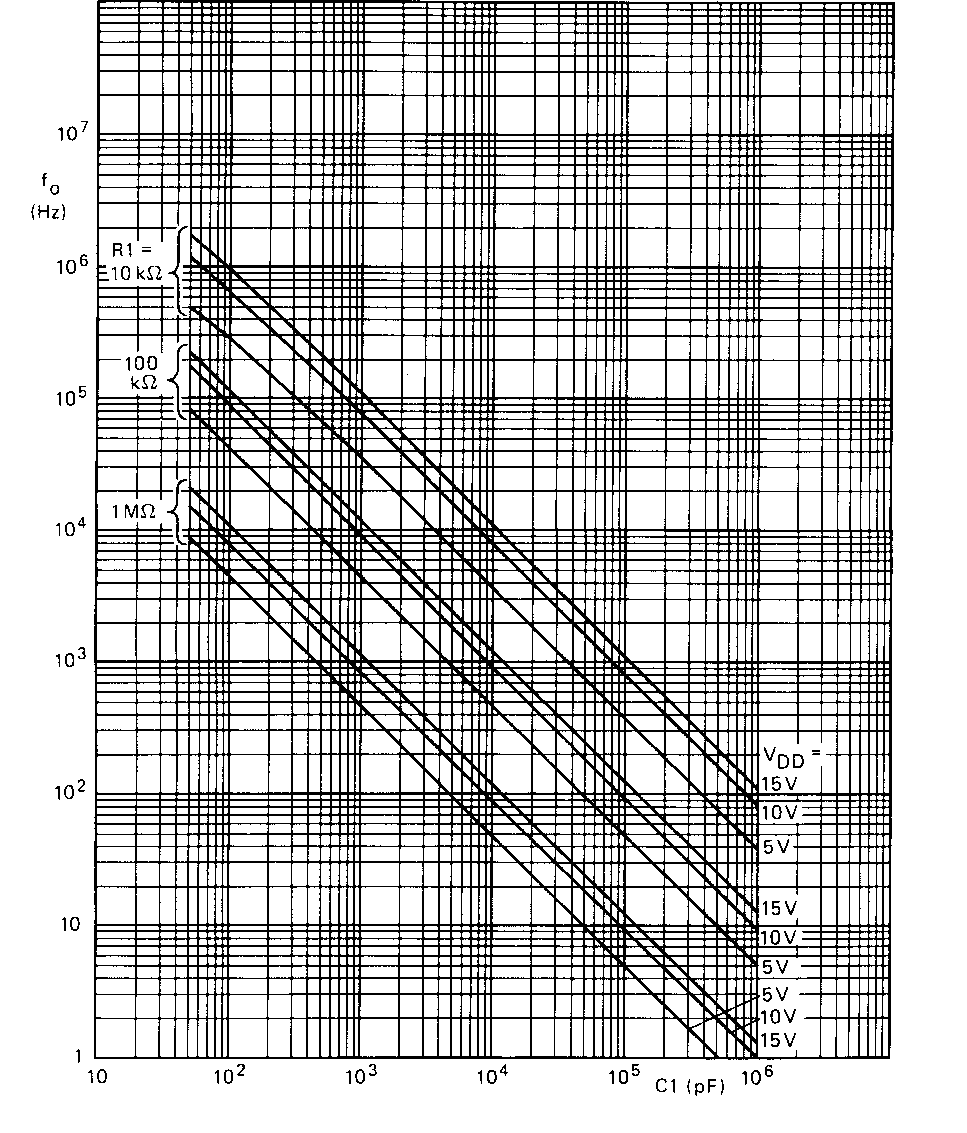
\includegraphics[scale=0.4]{report_img/4046graph}
		\caption{The capacitance used is determines the frequency of the signal produced. This graph, from the chip data sheet, allows the necessary capacitor to be chosen}
		\label{fig:4046graph}
	\end{center}
\end{figure}

Using trial and error, an optimum value for the capacitance was found at 2.8\,nF. In this arrangement, the maximum frequency that was available was measured and found to be 25600Hz and, similarly, the lowest frequency possible was 16.9\,Hz, shown in figure~\ref{fig:4046_high_low}. These are both outside audible range giving room for a decrease in range later. 

\begin{figure}[htbp]
	\centering
		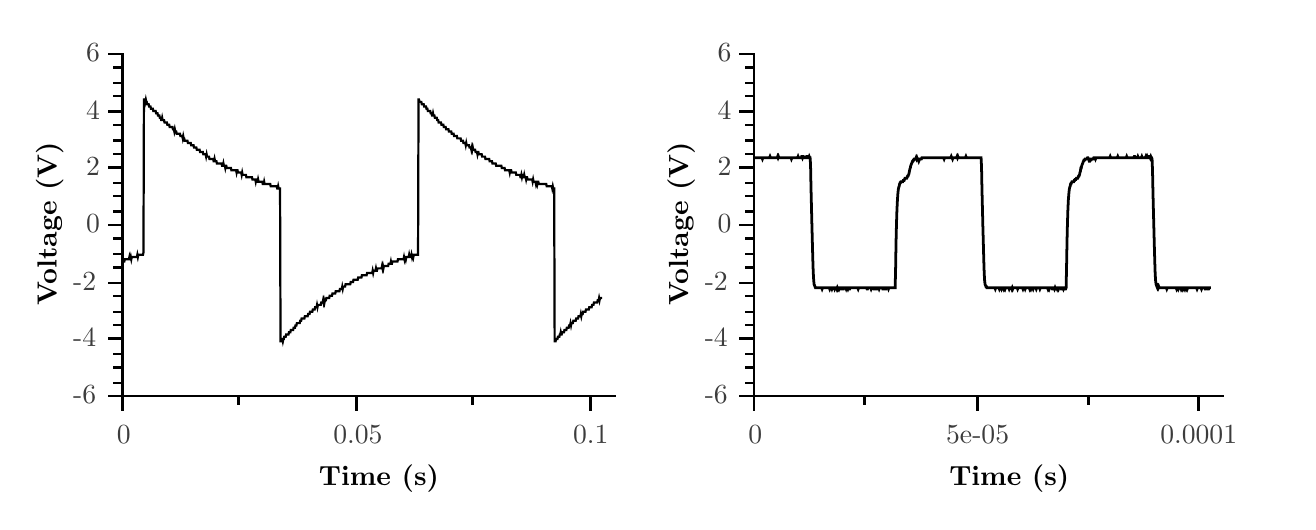
\begin{tikzpicture}{0pt}{0pt}{479pt}{180pt}
	\clip(0pt,180pt) -- (455.491pt,180pt) -- (455.491pt,8.83421pt) -- (0pt,8.83421pt) -- (0pt,180pt);
\begin{scope}
	\clip(262.454pt,170.491pt) -- (431.718pt,170.491pt) -- (431.718pt,46.8711pt) -- (262.454pt,46.8711pt) -- (262.454pt,170.491pt);
	\color[gray]{0}
	\draw[line width=1pt, line join=miter, line cap=rect](262.615pt,132.993pt) -- (262.776pt,132.993pt) -- (262.937pt,132.993pt) -- (263.098pt,132.993pt) -- (263.259pt,132.993pt) -- (263.42pt,132.993pt) -- (263.58pt,132.993pt) -- (263.741pt,132.993pt) -- (263.902pt,132.993pt) -- (264.063pt,132.993pt) -- (264.224pt,132.993pt) -- (264.385pt,132.993pt) -- (264.546pt,132.993pt) -- (264.707pt,132.993pt) -- (264.868pt,132.993pt) -- (265.029pt,132.993pt) -- (265.189pt,132.993pt) -- (265.35pt,132.993pt) -- (265.511pt,132.581pt) -- (265.672pt,132.993pt) -- (265.833pt,132.993pt) -- (265.994pt,132.993pt) -- (266.155pt,132.993pt) -- (266.316pt,132.993pt) -- (266.477pt,132.993pt) -- (266.638pt,132.993pt) -- (266.798pt,132.993pt) -- (266.959pt,132.993pt) -- (267.12pt,132.993pt) -- (267.281pt,132.993pt) -- (267.442pt,132.993pt) -- (267.603pt,132.993pt) -- (267.764pt,132.993pt) -- (267.925pt,132.993pt) -- (268.086pt,132.993pt) -- (268.247pt,133.405pt) -- (268.407pt,132.993pt) -- (268.568pt,132.993pt) -- (268.729pt,132.993pt) -- (268.89pt,132.993pt) -- (269.051pt,132.993pt) -- (269.212pt,132.993pt) -- (269.373pt,132.993pt) -- (269.534pt,132.993pt) -- (269.695pt,132.993pt) -- (269.855pt,132.993pt) -- (270.016pt,132.993pt) -- (270.177pt,132.993pt) -- (270.338pt,132.993pt) -- (270.499pt,132.993pt) -- (270.66pt,132.993pt) -- (270.821pt,132.993pt) -- (270.982pt,133.405pt) -- (271.143pt,132.993pt) -- (271.304pt,133.405pt) -- (271.464pt,132.993pt) -- (271.625pt,132.993pt) -- (271.786pt,132.993pt) -- (271.947pt,132.993pt) -- (272.108pt,132.993pt) -- (272.269pt,132.993pt) -- (272.43pt,132.993pt) -- (272.591pt,132.993pt) -- (272.752pt,132.993pt) -- (272.913pt,132.993pt) -- (273.073pt,132.993pt) -- (273.234pt,132.993pt) -- (273.395pt,132.993pt) -- (273.556pt,132.993pt) -- (273.717pt,132.993pt) -- (273.878pt,132.993pt) -- (274.039pt,132.993pt) -- (274.2pt,132.993pt) -- (274.361pt,132.993pt) -- (274.522pt,132.993pt) -- (274.682pt,132.993pt) -- (274.843pt,132.993pt) -- (275.004pt,132.993pt) -- (275.165pt,132.993pt) -- (275.326pt,132.993pt) -- (275.487pt,132.993pt) -- (275.648pt,132.993pt) -- (275.809pt,132.993pt) -- (275.97pt,132.581pt) -- (276.13pt,132.993pt) -- (276.291pt,132.993pt) -- (276.452pt,132.993pt) -- (276.613pt,132.993pt) -- (276.774pt,132.993pt) -- (276.935pt,132.993pt) -- (277.096pt,132.993pt) -- (277.257pt,132.993pt) -- (277.418pt,132.993pt) -- (277.579pt,132.993pt) -- (277.739pt,132.993pt) -- (277.9pt,132.993pt) -- (278.061pt,132.993pt) -- (278.222pt,132.993pt) -- (278.383pt,133.405pt) -- (278.544pt,132.993pt) -- (278.705pt,132.993pt) -- (278.866pt,132.993pt) -- (279.027pt,132.993pt) -- (279.188pt,132.993pt) -- (279.348pt,132.993pt) -- (279.509pt,132.993pt) -- (279.67pt,133.405pt) -- (279.831pt,133.405pt) -- (279.992pt,132.993pt) -- (280.153pt,133.405pt) -- (280.314pt,133.405pt) -- (280.475pt,132.993pt) -- (280.636pt,132.993pt) -- (280.797pt,132.993pt) -- (280.957pt,132.993pt) -- (281.118pt,132.993pt) -- (281.279pt,132.993pt) -- (281.44pt,133.405pt) -- (281.601pt,133.405pt) -- (281.762pt,133.405pt) -- (281.923pt,132.993pt) -- (282.084pt,132.993pt) -- (282.245pt,132.993pt) -- (282.405pt,133.405pt) -- (282.566pt,132.993pt) -- (282.727pt,132.993pt) -- (282.888pt,130.52pt) -- (283.049pt,122.279pt) -- (283.21pt,115.686pt) -- (283.371pt,109.093pt) -- (283.532pt,102.912pt) -- (283.693pt,96.731pt) -- (283.854pt,91.7862pt) -- (284.014pt,88.9018pt) -- (284.175pt,87.2535pt) -- (284.336pt,86.8414pt) -- (284.497pt,86.4294pt) -- (284.658pt,86.0173pt) -- (284.819pt,86.0173pt) -- (284.98pt,86.0173pt) -- (285.141pt,86.0173pt) -- (285.302pt,86.0173pt) -- (285.463pt,86.0173pt) -- (285.623pt,86.0173pt) -- (285.784pt,86.0173pt) -- (285.945pt,86.0173pt) -- (286.106pt,86.0173pt) -- (286.267pt,86.0173pt) -- (286.428pt,86.0173pt) -- (286.589pt,86.0173pt) -- (286.75pt,86.0173pt) -- (286.911pt,86.0173pt) -- (287.071pt,85.6052pt) -- (287.232pt,86.0173pt) -- (287.393pt,86.0173pt) -- (287.554pt,86.0173pt) -- (287.715pt,86.0173pt) -- (287.876pt,86.0173pt) -- (288.037pt,86.0173pt) -- (288.198pt,86.0173pt) -- (288.359pt,86.0173pt) -- (288.52pt,86.0173pt) -- (288.68pt,86.0173pt) -- (288.841pt,86.0173pt) -- (289.002pt,86.0173pt) -- (289.163pt,86.0173pt) -- (289.324pt,86.0173pt) -- (289.485pt,86.0173pt) -- (289.646pt,86.0173pt) -- (289.807pt,85.6052pt) -- (289.968pt,86.0173pt) -- (290.129pt,86.0173pt) -- (290.289pt,86.0173pt) -- (290.45pt,86.0173pt) -- (290.611pt,85.6052pt) -- (290.772pt,86.0173pt) -- (290.933pt,86.0173pt) -- (291.094pt,86.0173pt) -- (291.255pt,86.0173pt) -- (291.416pt,86.0173pt) -- (291.577pt,85.6052pt) -- (291.738pt,86.0173pt) -- (291.898pt,86.0173pt) -- (292.059pt,86.0173pt) -- (292.22pt,86.0173pt) -- (292.381pt,85.6052pt) -- (292.542pt,86.0173pt) -- (292.703pt,85.6052pt) -- (292.864pt,86.0173pt) -- (293.025pt,86.0173pt) -- (293.186pt,85.6052pt) -- (293.346pt,86.0173pt) -- (293.507pt,86.0173pt) -- (293.668pt,85.6052pt) -- (293.829pt,85.6052pt) -- (293.99pt,86.0173pt) -- (294.151pt,86.0173pt) -- (294.312pt,86.0173pt) -- (294.473pt,85.6052pt) -- (294.634pt,85.6052pt) -- (294.795pt,85.6052pt) -- (294.955pt,86.0173pt) -- (295.116pt,86.0173pt) -- (295.277pt,86.0173pt) -- (295.438pt,86.0173pt) -- (295.599pt,86.0173pt) -- (295.76pt,85.6052pt) -- (295.921pt,86.0173pt) -- (296.082pt,86.0173pt) -- (296.243pt,86.0173pt) -- (296.404pt,85.6052pt) -- (296.564pt,86.0173pt) -- (296.725pt,86.0173pt) -- (296.886pt,85.6052pt) -- (297.047pt,85.6052pt) -- (297.208pt,86.0173pt) -- (297.369pt,86.0173pt) -- (297.53pt,86.0173pt) -- (297.691pt,86.0173pt) -- (297.852pt,86.0173pt) -- (298.013pt,86.0173pt) -- (298.173pt,86.0173pt) -- (298.334pt,86.0173pt) -- (298.495pt,86.0173pt) -- (298.656pt,86.0173pt) -- (298.817pt,86.0173pt) -- (298.978pt,86.0173pt) -- (299.139pt,86.0173pt) -- (299.3pt,86.0173pt) -- (299.461pt,86.0173pt) -- (299.621pt,86.0173pt) -- (299.782pt,86.0173pt) -- (299.943pt,86.0173pt) -- (300.104pt,85.6052pt) -- (300.265pt,86.0173pt) -- (300.426pt,86.0173pt) -- (300.587pt,86.0173pt) -- (300.748pt,86.0173pt) -- (300.909pt,86.0173pt) -- (301.07pt,86.0173pt) -- (301.23pt,86.0173pt) -- (301.391pt,86.0173pt) -- (301.552pt,86.0173pt) -- (301.713pt,86.0173pt) -- (301.874pt,86.0173pt) -- (302.035pt,86.0173pt) -- (302.196pt,86.0173pt) -- (302.357pt,86.0173pt) -- (302.518pt,86.0173pt) -- (302.679pt,86.0173pt) -- (302.839pt,86.0173pt) -- (303pt,86.0173pt) -- (303.161pt,86.0173pt) -- (303.322pt,85.6052pt) -- (303.483pt,85.6052pt) -- (303.644pt,86.0173pt) -- (303.805pt,86.0173pt) -- (303.966pt,86.0173pt) -- (304.127pt,86.0173pt) -- (304.288pt,86.0173pt) -- (304.448pt,86.0173pt) -- (304.609pt,86.0173pt) -- (304.77pt,85.6052pt) -- (304.931pt,86.0173pt) -- (305.092pt,86.0173pt) -- (305.253pt,86.0173pt) -- (305.414pt,86.0173pt) -- (305.575pt,86.0173pt) -- (305.736pt,85.6052pt) -- (305.896pt,85.6052pt) -- (306.057pt,86.0173pt) -- (306.218pt,86.0173pt) -- (306.379pt,86.0173pt) -- (306.54pt,86.0173pt) -- (306.701pt,85.6052pt) -- (306.862pt,85.6052pt) -- (307.023pt,86.0173pt) -- (307.184pt,86.0173pt) -- (307.345pt,86.0173pt) -- (307.505pt,86.0173pt) -- (307.666pt,85.6052pt) -- (307.827pt,86.0173pt) -- (307.988pt,86.0173pt) -- (308.149pt,86.0173pt) -- (308.31pt,86.0173pt) -- (308.471pt,86.0173pt) -- (308.632pt,86.0173pt) -- (308.793pt,86.0173pt) -- (308.954pt,85.6052pt) -- (309.114pt,85.6052pt) -- (309.275pt,85.6052pt) -- (309.436pt,86.0173pt) -- (309.597pt,86.0173pt) -- (309.758pt,86.0173pt) -- (309.919pt,85.6052pt) -- (310.08pt,85.6052pt) -- (310.241pt,86.0173pt) -- (310.402pt,86.0173pt) -- (310.562pt,86.0173pt) -- (310.723pt,86.0173pt) -- (310.884pt,86.0173pt) -- (311.045pt,85.6052pt) -- (311.206pt,86.0173pt) -- (311.367pt,86.0173pt) -- (311.528pt,86.0173pt) -- (311.689pt,86.0173pt) -- (311.85pt,86.0173pt) -- (312.011pt,86.0173pt) -- (312.171pt,86.0173pt) -- (312.332pt,86.0173pt) -- (312.493pt,86.0173pt) -- (312.654pt,86.0173pt) -- (312.815pt,86.0173pt) -- (312.976pt,86.0173pt) -- (313.137pt,86.0173pt) -- (313.298pt,86.0173pt) -- (313.459pt,86.0173pt) -- (313.62pt,92.6104pt) -- (313.78pt,102.5pt) -- (313.941pt,109.093pt) -- (314.102pt,114.038pt) -- (314.263pt,117.334pt) -- (314.424pt,119.807pt) -- (314.585pt,121.455pt) -- (314.746pt,122.279pt) -- (314.907pt,122.691pt) -- (315.068pt,123.515pt) -- (315.229pt,123.927pt) -- (315.389pt,123.927pt) -- (315.55pt,124.339pt) -- (315.711pt,124.339pt) -- (315.872pt,124.339pt) -- (316.033pt,124.339pt) -- (316.194pt,124.339pt) -- (316.355pt,124.751pt) -- (316.516pt,124.751pt) -- (316.677pt,124.751pt) -- (316.837pt,125.164pt) -- (316.998pt,125.576pt) -- (317.159pt,125.576pt) -- (317.32pt,125.576pt) -- (317.481pt,125.576pt) -- (317.642pt,125.576pt) -- (317.803pt,125.988pt) -- (317.964pt,126.4pt) -- (318.125pt,126.4pt) -- (318.286pt,126.812pt) -- (318.446pt,127.224pt) -- (318.607pt,128.048pt) -- (318.768pt,128.872pt) -- (318.929pt,129.284pt) -- (319.09pt,130.108pt) -- (319.251pt,130.52pt) -- (319.412pt,130.932pt) -- (319.573pt,131.345pt) -- (319.734pt,131.757pt) -- (319.895pt,131.757pt) -- (320.055pt,132.169pt) -- (320.216pt,132.169pt) -- (320.377pt,132.581pt) -- (320.538pt,132.581pt) -- (320.699pt,132.581pt) -- (320.86pt,132.581pt) -- (321.021pt,132.993pt) -- (321.182pt,132.581pt) -- (321.343pt,132.993pt) -- (321.504pt,132.581pt) -- (321.664pt,132.581pt) -- (321.825pt,132.169pt) -- (321.986pt,131.757pt) -- (322.147pt,132.169pt) -- (322.308pt,132.581pt) -- (322.469pt,132.581pt) -- (322.63pt,132.581pt) -- (322.791pt,132.581pt) -- (322.952pt,132.581pt) -- (323.112pt,132.993pt) -- (323.273pt,132.993pt) -- (323.434pt,132.993pt) -- (323.595pt,132.993pt) -- (323.756pt,132.993pt) -- (323.917pt,132.993pt) -- (324.078pt,132.993pt) -- (324.239pt,132.993pt) -- (324.4pt,132.993pt) -- (324.561pt,132.993pt) -- (324.721pt,132.993pt) -- (324.882pt,132.993pt) -- (325.043pt,132.993pt) -- (325.204pt,132.993pt) -- (325.365pt,132.993pt) -- (325.526pt,132.993pt) -- (325.687pt,132.993pt) -- (325.848pt,132.993pt) -- (326.009pt,132.993pt) -- (326.17pt,132.993pt) -- (326.33pt,132.993pt) -- (326.491pt,132.993pt) -- (326.652pt,132.993pt) -- (326.813pt,132.993pt) -- (326.974pt,132.993pt) -- (327.135pt,132.993pt) -- (327.296pt,132.993pt) -- (327.457pt,132.993pt) -- (327.618pt,132.993pt) -- (327.779pt,132.993pt) -- (327.939pt,132.993pt) -- (328.1pt,132.993pt) -- (328.261pt,132.993pt) -- (328.422pt,132.993pt) -- (328.583pt,132.993pt) -- (328.744pt,132.993pt) -- (328.905pt,132.993pt) -- (329.066pt,132.993pt) -- (329.227pt,132.993pt) -- (329.387pt,132.993pt) -- (329.548pt,132.993pt) -- (329.709pt,132.993pt) -- (329.87pt,132.993pt) -- (330.031pt,132.993pt) -- (330.192pt,132.993pt) -- (330.353pt,132.993pt) -- (330.514pt,132.993pt) -- (330.675pt,132.993pt) -- (330.836pt,132.993pt) -- (330.996pt,132.993pt) -- (331.157pt,132.581pt) -- (331.318pt,132.993pt) -- (331.479pt,132.993pt) -- (331.64pt,132.993pt) -- (331.801pt,132.993pt) -- (331.962pt,132.993pt) -- (332.123pt,132.993pt) -- (332.284pt,132.993pt) -- (332.445pt,132.993pt) -- (332.605pt,132.993pt) -- (332.766pt,132.993pt) -- (332.927pt,132.993pt) -- (333.088pt,132.993pt) -- (333.249pt,132.993pt) -- (333.41pt,132.993pt) -- (333.571pt,132.993pt) -- (333.732pt,133.405pt) -- (333.893pt,132.993pt) -- (334.054pt,132.993pt) -- (334.214pt,132.581pt) -- (334.375pt,132.993pt) -- (334.536pt,132.993pt) -- (334.697pt,132.993pt) -- (334.858pt,132.993pt) -- (335.019pt,132.993pt) -- (335.18pt,132.993pt) -- (335.341pt,132.993pt) -- (335.502pt,132.993pt) -- (335.662pt,132.993pt) -- (335.823pt,133.405pt) -- (335.984pt,132.993pt) -- (336.145pt,133.405pt) -- (336.306pt,132.993pt) -- (336.467pt,132.993pt) -- (336.628pt,132.993pt) -- (336.789pt,132.993pt) -- (336.95pt,132.993pt) -- (337.111pt,132.993pt) -- (337.271pt,132.993pt) -- (337.432pt,132.993pt) -- (337.593pt,132.993pt) -- (337.754pt,132.993pt) -- (337.915pt,132.993pt) -- (338.076pt,132.993pt) -- (338.237pt,132.993pt) -- (338.398pt,132.993pt) -- (338.559pt,132.993pt) -- (338.72pt,132.993pt) -- (338.88pt,132.993pt) -- (339.041pt,133.405pt) -- (339.202pt,132.993pt) -- (339.363pt,132.993pt) -- (339.524pt,132.993pt) -- (339.685pt,132.993pt) -- (339.846pt,132.993pt) -- (340.007pt,132.993pt) -- (340.168pt,132.993pt) -- (340.328pt,132.993pt) -- (340.489pt,132.993pt) -- (340.65pt,132.993pt) -- (340.811pt,132.993pt) -- (340.972pt,132.993pt) -- (341.133pt,132.993pt) -- (341.294pt,132.993pt) -- (341.455pt,132.993pt) -- (341.616pt,132.993pt) -- (341.777pt,132.993pt) -- (341.937pt,132.993pt) -- (342.098pt,132.993pt) -- (342.259pt,132.993pt) -- (342.42pt,132.993pt) -- (342.581pt,132.993pt) -- (342.742pt,132.993pt) -- (342.903pt,132.993pt) -- (343.064pt,132.993pt) -- (343.225pt,132.993pt) -- (343.386pt,132.993pt) -- (343.546pt,132.993pt) -- (343.707pt,132.993pt) -- (343.868pt,132.993pt) -- (344.029pt,132.993pt) -- (344.19pt,132.993pt) -- (344.351pt,132.993pt) -- (344.512pt,132.993pt) -- (344.673pt,129.696pt) -- (344.834pt,121.455pt) -- (344.995pt,114.862pt) -- (345.155pt,108.269pt) -- (345.316pt,102.5pt) -- (345.477pt,96.3189pt) -- (345.638pt,91.3742pt) -- (345.799pt,88.4897pt) -- (345.96pt,87.2535pt) -- (346.121pt,86.8414pt) -- (346.282pt,86.4294pt) -- (346.443pt,86.4294pt) -- (346.603pt,86.0173pt) -- (346.764pt,86.0173pt) -- (346.925pt,86.0173pt) -- (347.086pt,86.0173pt) -- (347.247pt,86.0173pt) -- (347.408pt,86.0173pt) -- (347.569pt,86.0173pt) -- (347.73pt,86.0173pt) -- (347.891pt,86.0173pt) -- (348.052pt,86.0173pt) -- (348.212pt,86.0173pt) -- (348.373pt,86.0173pt) -- (348.534pt,86.0173pt) -- (348.695pt,86.0173pt) -- (348.856pt,86.0173pt) -- (349.017pt,86.0173pt) -- (349.178pt,86.0173pt) -- (349.339pt,86.0173pt) -- (349.5pt,86.0173pt) -- (349.661pt,85.6052pt) -- (349.821pt,86.0173pt) -- (349.982pt,86.0173pt) -- (350.143pt,86.0173pt) -- (350.304pt,86.0173pt) -- (350.465pt,86.0173pt) -- (350.626pt,86.0173pt) -- (350.787pt,86.0173pt) -- (350.948pt,86.0173pt) -- (351.109pt,85.6052pt) -- (351.27pt,86.0173pt) -- (351.43pt,86.0173pt) -- (351.591pt,86.0173pt) -- (351.752pt,86.0173pt) -- (351.913pt,85.6052pt) -- (352.074pt,86.0173pt) -- (352.235pt,86.0173pt) -- (352.396pt,86.0173pt) -- (352.557pt,86.0173pt) -- (352.718pt,85.6052pt) -- (352.878pt,86.0173pt) -- (353.039pt,86.0173pt) -- (353.2pt,85.6052pt) -- (353.361pt,86.0173pt) -- (353.522pt,86.0173pt) -- (353.683pt,86.0173pt) -- (353.844pt,86.0173pt) -- (354.005pt,86.0173pt) -- (354.166pt,86.0173pt) -- (354.327pt,86.0173pt) -- (354.487pt,86.0173pt) -- (354.648pt,85.6052pt) -- (354.809pt,86.0173pt) -- (354.97pt,86.0173pt) -- (355.131pt,86.0173pt) -- (355.292pt,86.0173pt) -- (355.453pt,86.0173pt) -- (355.614pt,85.6052pt) -- (355.775pt,86.0173pt) -- (355.936pt,85.6052pt) -- (356.096pt,86.0173pt) -- (356.257pt,86.0173pt) -- (356.418pt,86.0173pt) -- (356.579pt,86.0173pt) -- (356.74pt,86.0173pt) -- (356.901pt,86.0173pt) -- (357.062pt,86.0173pt) -- (357.223pt,86.0173pt) -- (357.384pt,86.0173pt) -- (357.545pt,86.0173pt) -- (357.705pt,85.6052pt) -- (357.866pt,86.0173pt) -- (358.027pt,86.0173pt) -- (358.188pt,86.0173pt) -- (358.349pt,86.0173pt) -- (358.51pt,86.0173pt) -- (358.671pt,86.0173pt) -- (358.832pt,86.0173pt) -- (358.993pt,86.0173pt) -- (359.153pt,86.0173pt) -- (359.314pt,86.0173pt) -- (359.475pt,86.0173pt) -- (359.636pt,85.6052pt) -- (359.797pt,86.0173pt) -- (359.958pt,86.0173pt) -- (360.119pt,86.0173pt) -- (360.28pt,86.0173pt) -- (360.441pt,85.6052pt) -- (360.602pt,86.0173pt) -- (360.762pt,86.0173pt) -- (360.923pt,86.0173pt) -- (361.084pt,86.0173pt) -- (361.245pt,86.0173pt) -- (361.406pt,86.0173pt) -- (361.567pt,86.0173pt) -- (361.728pt,86.0173pt) -- (361.889pt,86.0173pt) -- (362.05pt,85.6052pt) -- (362.211pt,86.0173pt) -- (362.371pt,86.0173pt) -- (362.532pt,85.6052pt) -- (362.693pt,86.0173pt) -- (362.854pt,86.0173pt) -- (363.015pt,86.0173pt) -- (363.176pt,86.0173pt) -- (363.337pt,85.6052pt) -- (363.498pt,86.0173pt) -- (363.659pt,86.0173pt) -- (363.82pt,86.0173pt) -- (363.98pt,86.0173pt) -- (364.141pt,86.0173pt) -- (364.302pt,86.0173pt) -- (364.463pt,85.6052pt) -- (364.624pt,86.0173pt) -- (364.785pt,86.0173pt) -- (364.946pt,86.0173pt) -- (365.107pt,86.0173pt) -- (365.268pt,86.0173pt) -- (365.428pt,86.0173pt) -- (365.589pt,86.0173pt) -- (365.75pt,85.6052pt) -- (365.911pt,86.0173pt) -- (366.072pt,86.0173pt) -- (366.233pt,86.0173pt) -- (366.394pt,86.0173pt) -- (366.555pt,86.0173pt) -- (366.716pt,86.0173pt) -- (366.877pt,86.0173pt) -- (367.037pt,86.0173pt) -- (367.198pt,86.0173pt) -- (367.359pt,86.0173pt) -- (367.52pt,86.0173pt) -- (367.681pt,86.0173pt) -- (367.842pt,86.0173pt) -- (368.003pt,86.0173pt) -- (368.164pt,86.0173pt) -- (368.325pt,86.0173pt) -- (368.486pt,86.0173pt) -- (368.646pt,85.6052pt) -- (368.807pt,86.0173pt) -- (368.968pt,86.0173pt) -- (369.129pt,85.6052pt) -- (369.29pt,86.0173pt) -- (369.451pt,86.0173pt) -- (369.612pt,86.0173pt) -- (369.773pt,86.0173pt) -- (369.934pt,86.0173pt) -- (370.094pt,86.0173pt) -- (370.255pt,85.6052pt) -- (370.416pt,85.6052pt) -- (370.577pt,86.0173pt) -- (370.738pt,86.0173pt) -- (370.899pt,86.0173pt) -- (371.06pt,85.6052pt) -- (371.221pt,86.0173pt) -- (371.382pt,85.6052pt) -- (371.543pt,85.6052pt) -- (371.703pt,86.0173pt) -- (371.864pt,86.0173pt) -- (372.025pt,85.6052pt) -- (372.186pt,86.0173pt) -- (372.347pt,86.0173pt) -- (372.508pt,85.6052pt) -- (372.669pt,86.0173pt) -- (372.83pt,86.0173pt) -- (372.991pt,86.0173pt) -- (373.152pt,86.0173pt) -- (373.312pt,86.0173pt) -- (373.473pt,85.6052pt) -- (373.634pt,85.6052pt) -- (373.795pt,86.0173pt) -- (373.956pt,86.0173pt) -- (374.117pt,86.0173pt) -- (374.278pt,85.6052pt) -- (374.439pt,86.0173pt) -- (374.6pt,86.0173pt) -- (374.761pt,86.0173pt) -- (374.921pt,85.6052pt) -- (375.082pt,85.6052pt) -- (375.243pt,86.0173pt) -- (375.404pt,93.8466pt) -- (375.565pt,102.912pt) -- (375.726pt,109.505pt) -- (375.887pt,114.45pt) -- (376.048pt,117.746pt) -- (376.209pt,119.807pt) -- (376.369pt,121.455pt) -- (376.53pt,122.279pt) -- (376.691pt,122.691pt) -- (376.852pt,123.515pt) -- (377.013pt,123.515pt) -- (377.174pt,123.927pt) -- (377.335pt,124.339pt) -- (377.496pt,124.339pt) -- (377.657pt,124.339pt) -- (377.818pt,124.339pt) -- (377.978pt,124.339pt) -- (378.139pt,124.751pt) -- (378.3pt,124.751pt) -- (378.461pt,125.164pt) -- (378.622pt,125.164pt) -- (378.783pt,125.164pt) -- (378.944pt,125.576pt) -- (379.105pt,125.576pt) -- (379.266pt,125.576pt) -- (379.427pt,125.576pt) -- (379.587pt,125.988pt) -- (379.748pt,126.4pt) -- (379.909pt,126.4pt) -- (380.07pt,126.812pt) -- (380.231pt,127.636pt) -- (380.392pt,128.048pt) -- (380.553pt,129.284pt) -- (380.714pt,129.284pt) -- (380.875pt,130.108pt) -- (381.036pt,130.52pt) -- (381.196pt,130.932pt) -- (381.357pt,131.345pt) -- (381.518pt,131.757pt) -- (381.679pt,132.169pt) -- (381.84pt,132.169pt) -- (382.001pt,132.169pt) -- (382.162pt,132.581pt) -- (382.323pt,132.581pt) -- (382.484pt,132.581pt) -- (382.644pt,132.581pt) -- (382.805pt,132.581pt) -- (382.966pt,132.993pt) -- (383.127pt,132.993pt) -- (383.288pt,132.581pt) -- (383.449pt,132.581pt) -- (383.61pt,131.757pt) -- (383.771pt,131.757pt) -- (383.932pt,132.169pt) -- (384.093pt,132.169pt) -- (384.253pt,132.169pt) -- (384.414pt,132.581pt) -- (384.575pt,132.581pt) -- (384.736pt,132.581pt) -- (384.897pt,132.581pt) -- (385.058pt,132.581pt) -- (385.219pt,132.993pt) -- (385.38pt,132.993pt) -- (385.541pt,132.993pt) -- (385.702pt,132.993pt) -- (385.862pt,132.581pt) -- (386.023pt,132.993pt) -- (386.184pt,132.993pt) -- (386.345pt,132.993pt) -- (386.506pt,132.993pt) -- (386.667pt,132.993pt) -- (386.828pt,132.993pt) -- (386.989pt,132.993pt) -- (387.15pt,132.993pt) -- (387.311pt,132.993pt) -- (387.471pt,132.993pt) -- (387.632pt,132.993pt) -- (387.793pt,132.993pt) -- (387.954pt,132.993pt) -- (388.115pt,132.993pt) -- (388.276pt,132.993pt) -- (388.437pt,132.993pt) -- (388.598pt,132.993pt) -- (388.759pt,132.993pt) -- (388.919pt,132.993pt) -- (389.08pt,132.993pt) -- (389.241pt,132.993pt) -- (389.402pt,132.993pt) -- (389.563pt,132.993pt) -- (389.724pt,132.993pt) -- (389.885pt,132.993pt) -- (390.046pt,132.993pt) -- (390.207pt,132.993pt) -- (390.368pt,132.993pt) -- (390.528pt,132.993pt) -- (390.689pt,132.993pt) -- (390.85pt,132.993pt) -- (391.011pt,132.993pt) -- (391.172pt,133.405pt) -- (391.333pt,132.993pt) -- (391.494pt,132.993pt) -- (391.655pt,132.993pt) -- (391.816pt,132.993pt) -- (391.977pt,132.993pt) -- (392.137pt,132.993pt) -- (392.298pt,132.993pt) -- (392.459pt,132.993pt) -- (392.62pt,132.993pt) -- (392.781pt,132.993pt) -- (392.942pt,132.993pt) -- (393.103pt,132.993pt) -- (393.264pt,132.993pt) -- (393.425pt,132.993pt) -- (393.586pt,132.993pt) -- (393.746pt,132.993pt) -- (393.907pt,133.405pt) -- (394.068pt,132.993pt) -- (394.229pt,132.993pt) -- (394.39pt,132.993pt) -- (394.551pt,132.993pt) -- (394.712pt,132.993pt) -- (394.873pt,132.993pt) -- (395.034pt,132.993pt) -- (395.194pt,132.993pt) -- (395.355pt,132.993pt) -- (395.516pt,132.993pt) -- (395.677pt,132.993pt) -- (395.838pt,132.993pt) -- (395.999pt,132.993pt) -- (396.16pt,132.993pt) -- (396.321pt,132.993pt) -- (396.482pt,132.993pt) -- (396.643pt,132.993pt) -- (396.803pt,132.993pt) -- (396.964pt,132.993pt) -- (397.125pt,133.405pt) -- (397.286pt,132.993pt) -- (397.447pt,132.993pt) -- (397.608pt,132.993pt) -- (397.769pt,132.993pt) -- (397.93pt,132.993pt) -- (398.091pt,132.993pt) -- (398.252pt,132.993pt) -- (398.412pt,132.993pt) -- (398.573pt,132.993pt) -- (398.734pt,132.993pt) -- (398.895pt,132.993pt) -- (399.056pt,132.993pt) -- (399.217pt,132.993pt) -- (399.378pt,132.993pt) -- (399.539pt,132.993pt) -- (399.7pt,132.993pt) -- (399.86pt,133.405pt) -- (400.021pt,133.405pt) -- (400.182pt,132.993pt) -- (400.343pt,132.993pt) -- (400.504pt,132.993pt) -- (400.665pt,132.993pt) -- (400.826pt,132.993pt) -- (400.987pt,132.993pt) -- (401.148pt,133.405pt) -- (401.309pt,132.993pt) -- (401.469pt,132.993pt) -- (401.63pt,132.993pt) -- (401.791pt,132.993pt) -- (401.952pt,132.993pt) -- (402.113pt,132.993pt) -- (402.274pt,132.993pt) -- (402.435pt,132.993pt) -- (402.596pt,133.405pt) -- (402.757pt,132.993pt) -- (402.918pt,132.993pt) -- (403.078pt,132.993pt) -- (403.239pt,132.993pt) -- (403.4pt,132.993pt) -- (403.561pt,132.993pt) -- (403.722pt,132.993pt) -- (403.883pt,132.993pt) -- (404.044pt,133.405pt) -- (404.205pt,132.993pt) -- (404.366pt,132.993pt) -- (404.527pt,133.405pt) -- (404.687pt,132.993pt) -- (404.848pt,132.993pt) -- (405.009pt,132.993pt) -- (405.17pt,133.405pt) -- (405.331pt,133.405pt) -- (405.492pt,133.405pt) -- (405.653pt,132.993pt) -- (405.814pt,133.405pt) -- (405.975pt,132.993pt) -- (406.135pt,132.993pt) -- (406.296pt,132.581pt) -- (406.457pt,128.46pt) -- (406.618pt,120.631pt) -- (406.779pt,114.038pt) -- (406.94pt,107.857pt) -- (407.101pt,101.676pt) -- (407.262pt,95.9069pt) -- (407.423pt,90.9621pt) -- (407.584pt,88.4897pt) -- (407.744pt,87.2535pt) -- (407.905pt,86.8414pt) -- (408.066pt,86.4294pt) -- (408.227pt,86.0173pt) -- (408.388pt,86.4294pt) -- (408.549pt,86.0173pt) -- (408.71pt,86.4294pt) -- (408.871pt,86.0173pt) -- (409.032pt,86.0173pt) -- (409.193pt,86.0173pt) -- (409.353pt,86.0173pt) -- (409.514pt,86.0173pt) -- (409.675pt,86.0173pt) -- (409.836pt,86.0173pt) -- (409.997pt,86.0173pt) -- (410.158pt,86.0173pt) -- (410.319pt,86.0173pt) -- (410.48pt,86.0173pt) -- (410.641pt,86.0173pt) -- (410.802pt,86.0173pt) -- (410.962pt,86.0173pt) -- (411.123pt,86.0173pt) -- (411.284pt,86.0173pt) -- (411.445pt,86.0173pt) -- (411.606pt,85.6052pt) -- (411.767pt,86.0173pt) -- (411.928pt,86.0173pt) -- (412.089pt,86.0173pt) -- (412.25pt,86.0173pt) -- (412.41pt,86.0173pt) -- (412.571pt,86.0173pt) -- (412.732pt,86.0173pt) -- (412.893pt,86.0173pt) -- (413.054pt,86.0173pt) -- (413.215pt,86.0173pt) -- (413.376pt,86.0173pt) -- (413.537pt,86.0173pt) -- (413.698pt,86.0173pt) -- (413.859pt,86.0173pt) -- (414.019pt,86.0173pt) -- (414.18pt,86.0173pt) -- (414.341pt,86.0173pt) -- (414.502pt,86.0173pt) -- (414.663pt,86.0173pt) -- (414.824pt,86.0173pt) -- (414.985pt,86.0173pt) -- (415.146pt,85.6052pt) -- (415.307pt,86.0173pt) -- (415.468pt,86.0173pt) -- (415.628pt,86.0173pt) -- (415.789pt,85.6052pt) -- (415.95pt,86.0173pt) -- (416.111pt,86.0173pt) -- (416.272pt,86.0173pt) -- (416.433pt,86.0173pt) -- (416.594pt,86.0173pt) -- (416.755pt,85.6052pt) -- (416.916pt,86.0173pt) -- (417.077pt,86.0173pt) -- (417.237pt,85.6052pt) -- (417.398pt,86.0173pt) -- (417.559pt,86.0173pt) -- (417.72pt,86.0173pt) -- (417.881pt,85.6052pt) -- (418.042pt,86.0173pt) -- (418.203pt,86.0173pt) -- (418.364pt,86.0173pt) -- (418.525pt,85.6052pt) -- (418.685pt,86.0173pt) -- (418.846pt,86.0173pt) -- (419.007pt,85.6052pt) -- (419.168pt,86.0173pt) -- (419.329pt,86.0173pt) -- (419.49pt,86.0173pt) -- (419.651pt,86.0173pt) -- (419.812pt,86.0173pt) -- (419.973pt,86.0173pt) -- (420.134pt,86.0173pt) -- (420.294pt,86.0173pt) -- (420.455pt,86.0173pt) -- (420.616pt,86.0173pt) -- (420.777pt,86.0173pt) -- (420.938pt,86.0173pt) -- (421.099pt,86.0173pt) -- (421.26pt,86.0173pt) -- (421.421pt,86.0173pt) -- (421.582pt,86.0173pt) -- (421.743pt,86.0173pt) -- (421.903pt,86.0173pt) -- (422.064pt,86.0173pt) -- (422.225pt,86.0173pt) -- (422.386pt,86.0173pt) -- (422.547pt,85.6052pt) -- (422.708pt,86.0173pt) -- (422.869pt,86.0173pt) -- (423.03pt,86.0173pt) -- (423.191pt,86.0173pt) -- (423.351pt,86.0173pt) -- (423.512pt,86.0173pt) -- (423.673pt,86.0173pt) -- (423.834pt,86.0173pt) -- (423.995pt,86.0173pt) -- (424.156pt,85.6052pt) -- (424.317pt,86.0173pt) -- (424.478pt,86.0173pt) -- (424.639pt,86.0173pt) -- (424.8pt,86.0173pt) -- (424.96pt,86.0173pt) -- (425.121pt,86.0173pt) -- (425.282pt,86.0173pt) -- (425.443pt,85.6052pt) -- (425.604pt,85.6052pt) -- (425.765pt,86.0173pt) -- (425.926pt,86.0173pt) -- (426.087pt,86.0173pt) -- (426.248pt,86.0173pt) -- (426.409pt,85.6052pt) -- (426.569pt,85.6052pt) -- (426.73pt,85.6052pt) -- (426.891pt,86.0173pt) -- (427.052pt,86.0173pt);
\end{scope}
\begin{scope}
	\color[gray]{0}
	\pgftext[center, base, at={\pgfpoint{238.681pt}{109.156pt}},rotate=90]{\textbf{Voltage (V)}}
	\color[gray]{0.235294}
	\pgftext[center, base, at={\pgfpoint{248.829pt}{44.0183pt}}]{-6}
	\pgftext[center, base, at={\pgfpoint{248.829pt}{64.9386pt}}]{-4}
	\pgftext[center, base, at={\pgfpoint{248.829pt}{84.9079pt}}]{-2}
	\pgftext[center, base, at={\pgfpoint{251.838pt}{105.828pt}}]{0}
	\pgftext[center, base, at={\pgfpoint{251.838pt}{126.748pt}}]{2}
	\pgftext[center, base, at={\pgfpoint{251.838pt}{146.718pt}}]{4}
	\pgftext[center, base, at={\pgfpoint{251.838pt}{167.638pt}}]{6}
	\color[gray]{0}
	\draw[line width=1pt, line join=bevel, line cap=rect](262.454pt,51.6257pt) -- (259.601pt,51.6257pt);
	\draw[line width=1pt, line join=bevel, line cap=rect](262.454pt,62.0858pt) -- (259.601pt,62.0858pt);
	\draw[line width=1pt, line join=bevel, line cap=rect](262.454pt,72.5459pt) -- (259.601pt,72.5459pt);
	\draw[line width=1pt, line join=bevel, line cap=rect](262.454pt,83.0061pt) -- (259.601pt,83.0061pt);
	\draw[line width=1pt, line join=bevel, line cap=rect](262.454pt,93.4662pt) -- (259.601pt,93.4662pt);
	\draw[line width=1pt, line join=bevel, line cap=rect](262.454pt,103.926pt) -- (259.601pt,103.926pt);
	\draw[line width=1pt, line join=bevel, line cap=rect](262.454pt,113.436pt) -- (259.601pt,113.436pt);
	\draw[line width=1pt, line join=bevel, line cap=rect](262.454pt,123.896pt) -- (259.601pt,123.896pt);
	\draw[line width=1pt, line join=bevel, line cap=rect](262.454pt,134.356pt) -- (259.601pt,134.356pt);
	\draw[line width=1pt, line join=bevel, line cap=rect](262.454pt,144.816pt) -- (259.601pt,144.816pt);
	\draw[line width=1pt, line join=bevel, line cap=rect](262.454pt,155.276pt) -- (259.601pt,155.276pt);
	\draw[line width=1pt, line join=bevel, line cap=rect](262.454pt,165.736pt) -- (259.601pt,165.736pt);
	\draw[line width=1pt, line join=bevel, line cap=rect](262.454pt,57.3312pt) -- (259.601pt,57.3312pt);
	\draw[line width=1pt, line join=bevel, line cap=rect](262.454pt,77.3005pt) -- (259.601pt,77.3005pt);
	\draw[line width=1pt, line join=bevel, line cap=rect](262.454pt,98.2208pt) -- (259.601pt,98.2208pt);
	\draw[line width=1pt, line join=bevel, line cap=rect](262.454pt,119.141pt) -- (259.601pt,119.141pt);
	\draw[line width=1pt, line join=bevel, line cap=rect](262.454pt,139.11pt) -- (259.601pt,139.11pt);
	\draw[line width=1pt, line join=bevel, line cap=rect](262.454pt,160.031pt) -- (259.601pt,160.031pt);
	\draw[line width=1pt, line join=bevel, line cap=rect](262.454pt,46.8711pt) -- (257.7pt,46.8711pt);
	\draw[line width=1pt, line join=bevel, line cap=rect](262.454pt,67.7913pt) -- (257.7pt,67.7913pt);
	\draw[line width=1pt, line join=bevel, line cap=rect](262.454pt,87.7607pt) -- (257.7pt,87.7607pt);
	\draw[line width=1pt, line join=bevel, line cap=rect](262.454pt,108.681pt) -- (257.7pt,108.681pt);
	\draw[line width=1pt, line join=bevel, line cap=rect](262.454pt,129.601pt) -- (257.7pt,129.601pt);
	\draw[line width=1pt, line join=bevel, line cap=rect](262.454pt,149.571pt) -- (257.7pt,149.571pt);
	\draw[line width=1pt, line join=bevel, line cap=rect](262.454pt,170.491pt) -- (257.7pt,170.491pt);
	\draw[line width=1pt, line join=bevel, line cap=rect](262.454pt,170.491pt) -- (262.454pt,46.8711pt);
	\pgftext[center, base, at={\pgfpoint{354.694pt}{14.5397pt}}]{\textbf{Time (s)}}
	\color[gray]{0.235294}
	\pgftext[center, base, at={\pgfpoint{262.922pt}{29.7545pt}}]{0}
	\pgftext[center, base, at={\pgfpoint{343.275pt}{29.7545pt}}]{5e-05}
	\pgftext[center, base, at={\pgfpoint{423.152pt}{29.7545pt}}]{0.0001}
	\color[gray]{0}
	\draw[line width=1pt, line join=bevel, line cap=rect](302.393pt,46.8711pt) -- (302.393pt,44.0183pt);
	\draw[line width=1pt, line join=bevel, line cap=rect](383.221pt,46.8711pt) -- (383.221pt,44.0183pt);
	\draw[line width=1pt, line join=bevel, line cap=rect](262.454pt,46.8711pt) -- (262.454pt,42.1164pt);
	\draw[line width=1pt, line join=bevel, line cap=rect](343.282pt,46.8711pt) -- (343.282pt,42.1164pt);
	\draw[line width=1pt, line join=bevel, line cap=rect](423.16pt,46.8711pt) -- (423.16pt,42.1164pt);
	\draw[line width=1pt, line join=bevel, line cap=rect](262.454pt,46.8711pt) -- (431.718pt,46.8711pt);
\end{scope}
\begin{scope}
	\clip(34.2332pt,170.491pt) -- (212.055pt,170.491pt) -- (212.055pt,46.8711pt) -- (34.2332pt,46.8711pt) -- (34.2332pt,170.491pt);
	\color[gray]{0}
	\draw[line width=0.8pt, line join=miter, line cap=rect](34.4022pt,95.4948pt) -- (34.5712pt,95.4948pt) -- (34.7403pt,95.4948pt) -- (34.9093pt,95.4948pt) -- (35.0783pt,96.3189pt) -- (35.2474pt,96.3189pt) -- (35.4164pt,96.3189pt) -- (35.5854pt,96.3189pt) -- (35.7545pt,96.3189pt) -- (35.9235pt,96.3189pt) -- (36.0925pt,96.3189pt) -- (36.2615pt,96.3189pt) -- (36.4306pt,96.3189pt) -- (36.5996pt,96.3189pt) -- (36.7686pt,97.1431pt) -- (36.9377pt,96.3189pt) -- (37.1067pt,96.3189pt) -- (37.2757pt,97.1431pt) -- (37.4448pt,96.3189pt) -- (37.6138pt,97.1431pt) -- (37.7828pt,97.1431pt) -- (37.9519pt,97.1431pt) -- (38.1209pt,97.1431pt) -- (38.2899pt,97.1431pt) -- (38.459pt,97.1431pt) -- (38.628pt,97.1431pt) -- (38.797pt,97.1431pt) -- (38.9661pt,97.1431pt) -- (39.1351pt,97.1431pt) -- (39.3041pt,97.1431pt) -- (39.4732pt,97.1431pt) -- (39.6422pt,97.9672pt) -- (39.8112pt,97.1431pt) -- (39.9803pt,97.9672pt) -- (40.1493pt,97.9672pt) -- (40.3183pt,97.9672pt) -- (40.4874pt,97.9672pt) -- (40.6564pt,97.9672pt) -- (40.8254pt,97.9672pt) -- (40.9945pt,97.9672pt) -- (41.1635pt,97.9672pt) -- (41.3325pt,97.9672pt) -- (41.5016pt,97.9672pt) -- (41.6706pt,97.9672pt) -- (41.8396pt,98.7913pt) -- (42.0087pt,154.008pt) -- (42.1777pt,154.008pt) -- (42.3467pt,154.008pt) -- (42.5158pt,153.184pt) -- (42.6848pt,154.008pt) -- (42.8538pt,153.184pt) -- (43.0229pt,153.184pt) -- (43.1919pt,152.36pt) -- (43.3609pt,152.36pt) -- (43.5299pt,152.36pt) -- (43.699pt,152.36pt) -- (43.868pt,151.536pt) -- (44.037pt,151.536pt) -- (44.2061pt,151.536pt) -- (44.3751pt,151.536pt) -- (44.5441pt,150.712pt) -- (44.7132pt,150.712pt) -- (44.8822pt,150.712pt) -- (45.0512pt,150.712pt) -- (45.2203pt,150.712pt) -- (45.3893pt,149.887pt) -- (45.5583pt,149.887pt) -- (45.7274pt,149.887pt) -- (45.8964pt,149.887pt) -- (46.0654pt,149.887pt) -- (46.2345pt,149.887pt) -- (46.4035pt,149.063pt) -- (46.5725pt,149.063pt) -- (46.7416pt,149.063pt) -- (46.9106pt,149.063pt) -- (47.0796pt,148.239pt) -- (47.2487pt,148.239pt) -- (47.4177pt,148.239pt) -- (47.5867pt,148.239pt) -- (47.7558pt,147.415pt) -- (47.9248pt,147.415pt) -- (48.0938pt,147.415pt) -- (48.2629pt,146.591pt) -- (48.4319pt,146.591pt) -- (48.6009pt,147.415pt) -- (48.77pt,146.591pt) -- (48.939pt,146.591pt) -- (49.108pt,146.591pt) -- (49.2771pt,146.591pt) -- (49.4461pt,145.767pt) -- (49.6151pt,145.767pt) -- (49.7842pt,145.767pt) -- (49.9532pt,145.767pt) -- (50.1222pt,145.767pt) -- (50.2912pt,145.767pt) -- (50.4603pt,144.943pt) -- (50.6293pt,144.943pt) -- (50.7983pt,144.943pt) -- (50.9674pt,144.943pt) -- (51.1364pt,144.943pt) -- (51.3054pt,144.119pt) -- (51.4745pt,144.119pt) -- (51.6435pt,144.119pt) -- (51.8125pt,144.119pt) -- (51.9816pt,144.119pt) -- (52.1506pt,144.119pt) -- (52.3196pt,144.119pt) -- (52.4887pt,143.294pt) -- (52.6577pt,143.294pt) -- (52.8267pt,143.294pt) -- (52.9958pt,142.47pt) -- (53.1648pt,143.294pt) -- (53.3338pt,142.47pt) -- (53.5029pt,142.47pt) -- (53.6719pt,142.47pt) -- (53.8409pt,141.646pt) -- (54.01pt,141.646pt) -- (54.179pt,141.646pt) -- (54.348pt,141.646pt) -- (54.5171pt,141.646pt) -- (54.6861pt,141.646pt) -- (54.8551pt,141.646pt) -- (55.0242pt,141.646pt) -- (55.1932pt,140.822pt) -- (55.3622pt,140.822pt) -- (55.5313pt,140.822pt) -- (55.7003pt,140.822pt) -- (55.8693pt,140.822pt) -- (56.0384pt,139.998pt) -- (56.2074pt,140.822pt) -- (56.3764pt,139.998pt) -- (56.5455pt,139.998pt) -- (56.7145pt,139.174pt) -- (56.8835pt,139.174pt) -- (57.0526pt,139.174pt) -- (57.2216pt,139.174pt) -- (57.3906pt,139.174pt) -- (57.5596pt,139.174pt) -- (57.7287pt,139.174pt) -- (57.8977pt,138.35pt) -- (58.0667pt,138.35pt) -- (58.2358pt,138.35pt) -- (58.4048pt,138.35pt) -- (58.5738pt,138.35pt) -- (58.7429pt,138.35pt) -- (58.9119pt,138.35pt) -- (59.0809pt,137.526pt) -- (59.25pt,137.526pt) -- (59.419pt,137.526pt) -- (59.588pt,137.526pt) -- (59.7571pt,137.526pt) -- (59.9261pt,137.526pt) -- (60.0951pt,136.701pt) -- (60.2642pt,136.701pt) -- (60.4332pt,136.701pt) -- (60.6022pt,136.701pt) -- (60.7713pt,136.701pt) -- (60.9403pt,136.701pt) -- (61.1093pt,135.877pt) -- (61.2784pt,135.877pt) -- (61.4474pt,135.877pt) -- (61.6164pt,135.877pt) -- (61.7855pt,135.877pt) -- (61.9545pt,135.877pt) -- (62.1235pt,135.877pt) -- (62.2926pt,135.053pt) -- (62.4616pt,135.053pt) -- (62.6306pt,135.053pt) -- (62.7997pt,135.053pt) -- (62.9687pt,135.053pt) -- (63.1377pt,135.053pt) -- (63.3068pt,135.053pt) -- (63.4758pt,134.229pt) -- (63.6448pt,134.229pt) -- (63.8139pt,134.229pt) -- (63.9829pt,134.229pt) -- (64.1519pt,134.229pt) -- (64.321pt,134.229pt) -- (64.49pt,133.405pt) -- (64.659pt,134.229pt) -- (64.828pt,133.405pt) -- (64.9971pt,133.405pt) -- (65.1661pt,133.405pt) -- (65.3351pt,133.405pt) -- (65.5042pt,133.405pt) -- (65.6732pt,132.581pt) -- (65.8422pt,132.581pt) -- (66.0113pt,132.581pt) -- (66.1803pt,132.581pt) -- (66.3493pt,132.581pt) -- (66.5184pt,132.581pt) -- (66.6874pt,132.581pt) -- (66.8564pt,132.581pt) -- (67.0255pt,132.581pt) -- (67.1945pt,131.757pt) -- (67.3635pt,131.757pt) -- (67.5326pt,132.581pt) -- (67.7016pt,131.757pt) -- (67.8706pt,131.757pt) -- (68.0397pt,131.757pt) -- (68.2087pt,131.757pt) -- (68.3777pt,130.932pt) -- (68.5468pt,130.932pt) -- (68.7158pt,130.932pt) -- (68.8848pt,130.932pt) -- (69.0539pt,130.932pt) -- (69.2229pt,130.932pt) -- (69.3919pt,130.932pt) -- (69.561pt,130.932pt) -- (69.73pt,130.932pt) -- (69.899pt,130.932pt) -- (70.0681pt,130.932pt) -- (70.2371pt,130.108pt) -- (70.4061pt,130.108pt) -- (70.5752pt,130.108pt) -- (70.7442pt,130.932pt) -- (70.9132pt,130.108pt) -- (71.0823pt,130.108pt) -- (71.2513pt,130.108pt) -- (71.4203pt,129.284pt) -- (71.5894pt,130.108pt) -- (71.7584pt,130.108pt) -- (71.9274pt,129.284pt) -- (72.0964pt,129.284pt) -- (72.2655pt,129.284pt) -- (72.4345pt,129.284pt) -- (72.6035pt,129.284pt) -- (72.7726pt,129.284pt) -- (72.9416pt,129.284pt) -- (73.1106pt,129.284pt) -- (73.2797pt,129.284pt) -- (73.4487pt,129.284pt) -- (73.6177pt,128.46pt) -- (73.7868pt,128.46pt) -- (73.9558pt,128.46pt) -- (74.1248pt,128.46pt) -- (74.2939pt,128.46pt) -- (74.4629pt,128.46pt) -- (74.6319pt,128.46pt) -- (74.801pt,128.46pt) -- (74.97pt,128.46pt) -- (75.139pt,128.46pt) -- (75.3081pt,128.46pt) -- (75.4771pt,127.636pt) -- (75.6461pt,128.46pt) -- (75.8152pt,128.46pt) -- (75.9842pt,127.636pt) -- (76.1532pt,127.636pt) -- (76.3223pt,127.636pt) -- (76.4913pt,127.636pt) -- (76.6603pt,127.636pt) -- (76.8294pt,127.636pt) -- (76.9984pt,127.636pt) -- (77.1674pt,127.636pt) -- (77.3365pt,126.812pt) -- (77.5055pt,127.636pt) -- (77.6745pt,126.812pt) -- (77.8436pt,126.812pt) -- (78.0126pt,126.812pt) -- (78.1816pt,126.812pt) -- (78.3507pt,126.812pt) -- (78.5197pt,126.812pt) -- (78.6887pt,126.812pt) -- (78.8577pt,126.812pt) -- (79.0268pt,125.988pt) -- (79.1958pt,125.988pt) -- (79.3648pt,125.988pt) -- (79.5339pt,125.988pt) -- (79.7029pt,125.988pt) -- (79.8719pt,125.988pt) -- (80.041pt,125.988pt) -- (80.21pt,125.988pt) -- (80.379pt,125.988pt) -- (80.5481pt,125.988pt) -- (80.7171pt,125.988pt) -- (80.8861pt,125.988pt) -- (81.0552pt,125.988pt) -- (81.2242pt,125.164pt) -- (81.3932pt,125.164pt) -- (81.5623pt,125.164pt) -- (81.7313pt,125.164pt) -- (81.9003pt,125.164pt) -- (82.0694pt,125.164pt) -- (82.2384pt,125.164pt) -- (82.4074pt,124.339pt) -- (82.5765pt,125.164pt) -- (82.7455pt,125.164pt) -- (82.9145pt,124.339pt) -- (83.0836pt,124.339pt) -- (83.2526pt,125.164pt) -- (83.4216pt,124.339pt) -- (83.5907pt,124.339pt) -- (83.7597pt,124.339pt) -- (83.9287pt,124.339pt) -- (84.0978pt,124.339pt) -- (84.2668pt,124.339pt) -- (84.4358pt,124.339pt) -- (84.6049pt,124.339pt) -- (84.7739pt,124.339pt) -- (84.9429pt,123.515pt) -- (85.112pt,123.515pt) -- (85.281pt,123.515pt) -- (85.45pt,124.339pt) -- (85.6191pt,123.515pt) -- (85.7881pt,123.515pt) -- (85.9571pt,123.515pt) -- (86.1261pt,123.515pt) -- (86.2952pt,123.515pt) -- (86.4642pt,123.515pt) -- (86.6332pt,123.515pt) -- (86.8023pt,123.515pt) -- (86.9713pt,123.515pt) -- (87.1403pt,123.515pt) -- (87.3094pt,123.515pt) -- (87.4784pt,123.515pt) -- (87.6474pt,123.515pt) -- (87.8165pt,122.691pt) -- (87.9855pt,122.691pt) -- (88.1545pt,122.691pt) -- (88.3236pt,122.691pt) -- (88.4926pt,122.691pt) -- (88.6616pt,122.691pt) -- (88.8307pt,122.691pt) -- (88.9997pt,122.691pt) -- (89.1687pt,122.691pt) -- (89.3378pt,122.691pt) -- (89.5068pt,122.691pt) -- (89.6758pt,122.691pt) -- (89.8449pt,122.691pt) -- (90.0139pt,122.691pt) -- (90.1829pt,121.867pt) -- (90.352pt,121.867pt) -- (90.521pt,122.691pt) -- (90.69pt,121.867pt) -- (90.8591pt,121.867pt) -- (91.0281pt,121.867pt) -- (91.1971pt,121.867pt) -- (91.3662pt,66.6502pt) -- (91.5352pt,66.6502pt) -- (91.7042pt,66.6502pt) -- (91.8733pt,67.4743pt) -- (92.0423pt,67.4743pt) -- (92.2113pt,66.6502pt) -- (92.3804pt,67.4743pt) -- (92.5494pt,67.4743pt) -- (92.7184pt,68.2985pt) -- (92.8875pt,68.2985pt) -- (93.0565pt,68.2985pt) -- (93.2255pt,68.2985pt) -- (93.3945pt,69.1226pt) -- (93.5636pt,69.1226pt) -- (93.7326pt,69.1226pt) -- (93.9016pt,69.1226pt) -- (94.0707pt,69.1226pt) -- (94.2397pt,69.1226pt) -- (94.4087pt,69.9467pt) -- (94.5778pt,69.9467pt) -- (94.7468pt,69.9467pt) -- (94.9158pt,69.9467pt) -- (95.0849pt,70.7709pt) -- (95.2539pt,70.7709pt) -- (95.4229pt,70.7709pt) -- (95.592pt,70.7709pt) -- (95.761pt,70.7709pt) -- (95.93pt,70.7709pt) -- (96.0991pt,71.595pt) -- (96.2681pt,71.595pt) -- (96.4371pt,71.595pt) -- (96.6062pt,71.595pt) -- (96.7752pt,72.4191pt) -- (96.9442pt,72.4191pt) -- (97.1133pt,72.4191pt) -- (97.2823pt,73.2433pt) -- (97.4513pt,73.2433pt) -- (97.6204pt,73.2433pt) -- (97.7894pt,73.2433pt) -- (97.9584pt,73.2433pt) -- (98.1275pt,73.2433pt) -- (98.2965pt,73.2433pt) -- (98.4655pt,74.0674pt) -- (98.6346pt,74.0674pt) -- (98.8036pt,74.0674pt) -- (98.9726pt,74.8915pt) -- (99.1417pt,74.8915pt) -- (99.3107pt,74.8915pt) -- (99.4797pt,74.8915pt) -- (99.6488pt,74.8915pt) -- (99.8178pt,74.8915pt) -- (99.9868pt,74.8915pt) -- (100.156pt,75.7157pt) -- (100.325pt,75.7157pt) -- (100.494pt,75.7157pt) -- (100.663pt,75.7157pt) -- (100.832pt,75.7157pt) -- (101.001pt,75.7157pt) -- (101.17pt,75.7157pt) -- (101.339pt,76.5398pt) -- (101.508pt,76.5398pt) -- (101.677pt,76.5398pt) -- (101.846pt,76.5398pt) -- (102.015pt,77.3639pt) -- (102.184pt,77.3639pt) -- (102.353pt,77.3639pt) -- (102.522pt,77.3639pt) -- (102.691pt,77.3639pt) -- (102.86pt,77.3639pt) -- (103.029pt,78.1881pt) -- (103.198pt,78.1881pt) -- (103.367pt,78.1881pt) -- (103.537pt,78.1881pt) -- (103.706pt,78.1881pt) -- (103.875pt,79.0122pt) -- (104.044pt,79.0122pt) -- (104.213pt,79.0122pt) -- (104.382pt,79.0122pt) -- (104.551pt,79.8363pt) -- (104.72pt,79.0122pt) -- (104.889pt,79.8363pt) -- (105.058pt,79.8363pt) -- (105.227pt,79.8363pt) -- (105.396pt,79.8363pt) -- (105.565pt,79.8363pt) -- (105.734pt,79.8363pt) -- (105.903pt,79.8363pt) -- (106.072pt,80.6604pt) -- (106.241pt,80.6604pt) -- (106.41pt,80.6604pt) -- (106.579pt,80.6604pt) -- (106.748pt,81.4846pt) -- (106.917pt,80.6604pt) -- (107.086pt,81.4846pt) -- (107.255pt,80.6604pt) -- (107.424pt,81.4846pt) -- (107.593pt,81.4846pt) -- (107.762pt,81.4846pt) -- (107.931pt,82.3087pt) -- (108.1pt,82.3087pt) -- (108.269pt,82.3087pt) -- (108.438pt,82.3087pt) -- (108.607pt,82.3087pt) -- (108.777pt,82.3087pt) -- (108.946pt,82.3087pt) -- (109.115pt,83.1328pt) -- (109.284pt,83.1328pt) -- (109.453pt,83.1328pt) -- (109.622pt,83.1328pt) -- (109.791pt,83.1328pt) -- (109.96pt,83.1328pt) -- (110.129pt,83.957pt) -- (110.298pt,83.957pt) -- (110.467pt,83.957pt) -- (110.636pt,83.957pt) -- (110.805pt,83.957pt) -- (110.974pt,83.957pt) -- (111.143pt,83.957pt) -- (111.312pt,84.7811pt) -- (111.481pt,84.7811pt) -- (111.65pt,84.7811pt) -- (111.819pt,84.7811pt) -- (111.988pt,84.7811pt) -- (112.157pt,84.7811pt) -- (112.326pt,84.7811pt) -- (112.495pt,84.7811pt) -- (112.664pt,84.7811pt) -- (112.833pt,85.6052pt) -- (113.002pt,85.6052pt) -- (113.171pt,85.6052pt) -- (113.34pt,85.6052pt) -- (113.509pt,85.6052pt) -- (113.678pt,86.4294pt) -- (113.847pt,85.6052pt) -- (114.017pt,86.4294pt) -- (114.186pt,86.4294pt) -- (114.355pt,86.4294pt) -- (114.524pt,86.4294pt) -- (114.693pt,86.4294pt) -- (114.862pt,87.2535pt) -- (115.031pt,87.2535pt) -- (115.2pt,87.2535pt) -- (115.369pt,87.2535pt) -- (115.538pt,87.2535pt) -- (115.707pt,87.2535pt) -- (115.876pt,87.2535pt) -- (116.045pt,87.2535pt) -- (116.214pt,87.2535pt) -- (116.383pt,87.2535pt) -- (116.552pt,87.2535pt) -- (116.721pt,88.0776pt) -- (116.89pt,88.0776pt) -- (117.059pt,88.0776pt) -- (117.228pt,88.0776pt) -- (117.397pt,88.0776pt) -- (117.566pt,88.0776pt) -- (117.735pt,88.9018pt) -- (117.904pt,88.9018pt) -- (118.073pt,88.9018pt) -- (118.242pt,88.9018pt) -- (118.411pt,88.9018pt) -- (118.58pt,88.9018pt) -- (118.749pt,88.9018pt) -- (118.918pt,88.9018pt) -- (119.087pt,88.9018pt) -- (119.257pt,88.9018pt) -- (119.426pt,89.7259pt) -- (119.595pt,89.7259pt) -- (119.764pt,89.7259pt) -- (119.933pt,89.7259pt) -- (120.102pt,89.7259pt) -- (120.271pt,89.7259pt) -- (120.44pt,89.7259pt) -- (120.609pt,89.7259pt) -- (120.778pt,90.55pt) -- (120.947pt,90.55pt) -- (121.116pt,90.55pt) -- (121.285pt,90.55pt) -- (121.454pt,90.55pt) -- (121.623pt,90.55pt) -- (121.792pt,90.55pt) -- (121.961pt,90.55pt) -- (122.13pt,90.55pt) -- (122.299pt,90.55pt) -- (122.468pt,90.55pt) -- (122.637pt,91.3742pt) -- (122.806pt,91.3742pt) -- (122.975pt,91.3742pt) -- (123.144pt,91.3742pt) -- (123.313pt,91.3742pt) -- (123.482pt,91.3742pt) -- (123.651pt,91.3742pt) -- (123.82pt,91.3742pt) -- (123.989pt,91.3742pt) -- (124.158pt,91.3742pt) -- (124.328pt,91.3742pt) -- (124.497pt,91.3742pt) -- (124.666pt,92.1983pt) -- (124.835pt,91.3742pt) -- (125.004pt,92.1983pt) -- (125.173pt,92.1983pt) -- (125.342pt,92.1983pt) -- (125.511pt,92.1983pt) -- (125.68pt,92.1983pt) -- (125.849pt,93.0224pt) -- (126.018pt,92.1983pt) -- (126.187pt,92.1983pt) -- (126.356pt,93.0224pt) -- (126.525pt,93.0224pt) -- (126.694pt,93.0224pt) -- (126.863pt,93.0224pt) -- (127.032pt,93.0224pt) -- (127.201pt,93.0224pt) -- (127.37pt,93.0224pt) -- (127.539pt,93.0224pt) -- (127.708pt,93.0224pt) -- (127.877pt,93.0224pt) -- (128.046pt,93.8466pt) -- (128.215pt,93.0224pt) -- (128.384pt,93.8466pt) -- (128.553pt,93.0224pt) -- (128.722pt,93.8466pt) -- (128.891pt,93.8466pt) -- (129.06pt,93.8466pt) -- (129.229pt,93.8466pt) -- (129.398pt,93.8466pt) -- (129.568pt,93.8466pt) -- (129.737pt,93.8466pt) -- (129.906pt,93.8466pt) -- (130.075pt,93.8466pt) -- (130.244pt,93.8466pt) -- (130.413pt,94.6707pt) -- (130.582pt,94.6707pt) -- (130.751pt,94.6707pt) -- (130.92pt,94.6707pt) -- (131.089pt,94.6707pt) -- (131.258pt,95.4948pt) -- (131.427pt,94.6707pt) -- (131.596pt,94.6707pt) -- (131.765pt,95.4948pt) -- (131.934pt,95.4948pt) -- (132.103pt,95.4948pt) -- (132.272pt,95.4948pt) -- (132.441pt,95.4948pt) -- (132.61pt,95.4948pt) -- (132.779pt,95.4948pt) -- (132.948pt,95.4948pt) -- (133.117pt,95.4948pt) -- (133.286pt,95.4948pt) -- (133.455pt,95.4948pt) -- (133.624pt,95.4948pt) -- (133.793pt,96.3189pt) -- (133.962pt,96.3189pt) -- (134.131pt,96.3189pt) -- (134.3pt,96.3189pt) -- (134.469pt,96.3189pt) -- (134.638pt,96.3189pt) -- (134.808pt,96.3189pt) -- (134.977pt,96.3189pt) -- (135.146pt,96.3189pt) -- (135.315pt,96.3189pt) -- (135.484pt,96.3189pt) -- (135.653pt,96.3189pt) -- (135.822pt,96.3189pt) -- (135.991pt,97.1431pt) -- (136.16pt,96.3189pt) -- (136.329pt,97.1431pt) -- (136.498pt,97.1431pt) -- (136.667pt,96.3189pt) -- (136.836pt,97.1431pt) -- (137.005pt,97.1431pt) -- (137.174pt,97.1431pt) -- (137.343pt,97.1431pt) -- (137.512pt,97.1431pt) -- (137.681pt,97.1431pt) -- (137.85pt,97.9672pt) -- (138.019pt,97.1431pt) -- (138.188pt,97.1431pt) -- (138.357pt,97.1431pt) -- (138.526pt,97.1431pt) -- (138.695pt,97.9672pt) -- (138.864pt,97.1431pt) -- (139.033pt,97.9672pt) -- (139.202pt,97.9672pt) -- (139.371pt,97.1431pt) -- (139.54pt,97.9672pt) -- (139.709pt,97.9672pt) -- (139.878pt,97.9672pt) -- (140.048pt,97.9672pt) -- (140.217pt,97.9672pt) -- (140.386pt,97.9672pt) -- (140.555pt,97.9672pt) -- (140.724pt,97.9672pt) -- (140.893pt,97.9672pt) -- (141.062pt,97.9672pt) -- (141.231pt,154.008pt) -- (141.4pt,154.008pt) -- (141.569pt,153.184pt) -- (141.738pt,153.184pt) -- (141.907pt,153.184pt) -- (142.076pt,153.184pt) -- (142.245pt,153.184pt) -- (142.414pt,152.36pt) -- (142.583pt,152.36pt) -- (142.752pt,152.36pt) -- (142.921pt,152.36pt) -- (143.09pt,152.36pt) -- (143.259pt,151.536pt) -- (143.428pt,151.536pt) -- (143.597pt,151.536pt) -- (143.766pt,151.536pt) -- (143.935pt,151.536pt) -- (144.104pt,150.712pt) -- (144.273pt,150.712pt) -- (144.442pt,150.712pt) -- (144.611pt,149.887pt) -- (144.78pt,149.887pt) -- (144.949pt,149.887pt) -- (145.119pt,149.887pt) -- (145.288pt,149.887pt) -- (145.457pt,149.887pt) -- (145.626pt,149.063pt) -- (145.795pt,149.063pt) -- (145.964pt,149.063pt) -- (146.133pt,148.239pt) -- (146.302pt,148.239pt) -- (146.471pt,149.063pt) -- (146.64pt,148.239pt) -- (146.809pt,148.239pt) -- (146.978pt,148.239pt) -- (147.147pt,147.415pt) -- (147.316pt,147.415pt) -- (147.485pt,147.415pt) -- (147.654pt,147.415pt) -- (147.823pt,147.415pt) -- (147.992pt,146.591pt) -- (148.161pt,146.591pt) -- (148.33pt,146.591pt) -- (148.499pt,145.767pt) -- (148.668pt,145.767pt) -- (148.837pt,145.767pt) -- (149.006pt,145.767pt) -- (149.175pt,145.767pt) -- (149.344pt,145.767pt) -- (149.513pt,144.943pt) -- (149.682pt,144.943pt) -- (149.851pt,144.943pt) -- (150.02pt,144.943pt) -- (150.189pt,144.943pt) -- (150.359pt,144.119pt) -- (150.528pt,144.119pt) -- (150.697pt,144.119pt) -- (150.866pt,144.119pt) -- (151.035pt,144.119pt) -- (151.204pt,143.294pt) -- (151.373pt,143.294pt) -- (151.542pt,143.294pt) -- (151.711pt,143.294pt) -- (151.88pt,143.294pt) -- (152.049pt,143.294pt) -- (152.218pt,142.47pt) -- (152.387pt,142.47pt) -- (152.556pt,142.47pt) -- (152.725pt,142.47pt) -- (152.894pt,142.47pt) -- (153.063pt,142.47pt) -- (153.232pt,141.646pt) -- (153.401pt,141.646pt) -- (153.57pt,141.646pt) -- (153.739pt,141.646pt) -- (153.908pt,141.646pt) -- (154.077pt,140.822pt) -- (154.246pt,140.822pt) -- (154.415pt,140.822pt) -- (154.584pt,140.822pt) -- (154.753pt,140.822pt) -- (154.922pt,140.822pt) -- (155.091pt,140.822pt) -- (155.26pt,139.998pt) -- (155.429pt,139.998pt) -- (155.599pt,139.998pt) -- (155.768pt,139.998pt) -- (155.937pt,139.998pt) -- (156.106pt,139.998pt) -- (156.275pt,139.998pt) -- (156.444pt,139.998pt) -- (156.613pt,139.174pt) -- (156.782pt,139.174pt) -- (156.951pt,139.174pt) -- (157.12pt,139.174pt) -- (157.289pt,139.174pt) -- (157.458pt,138.35pt) -- (157.627pt,138.35pt) -- (157.796pt,138.35pt) -- (157.965pt,138.35pt) -- (158.134pt,138.35pt) -- (158.303pt,137.526pt) -- (158.472pt,138.35pt) -- (158.641pt,137.526pt) -- (158.81pt,137.526pt) -- (158.979pt,137.526pt) -- (159.148pt,137.526pt) -- (159.317pt,137.526pt) -- (159.486pt,137.526pt) -- (159.655pt,136.701pt) -- (159.824pt,136.701pt) -- (159.993pt,136.701pt) -- (160.162pt,136.701pt) -- (160.331pt,135.877pt) -- (160.5pt,136.701pt) -- (160.67pt,135.877pt) -- (160.839pt,136.701pt) -- (161.008pt,135.877pt) -- (161.177pt,135.877pt) -- (161.346pt,135.877pt) -- (161.515pt,135.877pt) -- (161.684pt,135.877pt) -- (161.853pt,135.053pt) -- (162.022pt,135.053pt) -- (162.191pt,135.053pt) -- (162.36pt,135.053pt) -- (162.529pt,134.229pt) -- (162.698pt,135.053pt) -- (162.867pt,135.053pt) -- (163.036pt,134.229pt) -- (163.205pt,134.229pt) -- (163.374pt,134.229pt) -- (163.543pt,134.229pt) -- (163.712pt,134.229pt) -- (163.881pt,134.229pt) -- (164.05pt,134.229pt) -- (164.219pt,133.405pt) -- (164.388pt,133.405pt) -- (164.557pt,133.405pt) -- (164.726pt,133.405pt) -- (164.895pt,133.405pt) -- (165.064pt,133.405pt) -- (165.233pt,133.405pt) -- (165.402pt,132.581pt) -- (165.571pt,132.581pt) -- (165.74pt,132.581pt) -- (165.91pt,132.581pt) -- (166.079pt,132.581pt) -- (166.248pt,132.581pt) -- (166.417pt,132.581pt) -- (166.586pt,132.581pt) -- (166.755pt,132.581pt) -- (166.924pt,131.757pt) -- (167.093pt,131.757pt) -- (167.262pt,131.757pt) -- (167.431pt,131.757pt) -- (167.6pt,131.757pt) -- (167.769pt,131.757pt) -- (167.938pt,130.932pt) -- (168.107pt,130.932pt) -- (168.276pt,130.932pt) -- (168.445pt,130.932pt) -- (168.614pt,130.932pt) -- (168.783pt,130.932pt) -- (168.952pt,130.932pt) -- (169.121pt,130.932pt) -- (169.29pt,130.108pt) -- (169.459pt,130.108pt) -- (169.628pt,130.108pt) -- (169.797pt,130.108pt) -- (169.966pt,130.108pt) -- (170.135pt,130.108pt) -- (170.304pt,130.108pt) -- (170.473pt,130.108pt) -- (170.642pt,130.108pt) -- (170.811pt,130.108pt) -- (170.98pt,130.108pt) -- (171.15pt,130.108pt) -- (171.319pt,129.284pt) -- (171.488pt,129.284pt) -- (171.657pt,129.284pt) -- (171.826pt,129.284pt) -- (171.995pt,129.284pt) -- (172.164pt,129.284pt) -- (172.333pt,129.284pt) -- (172.502pt,128.46pt) -- (172.671pt,128.46pt) -- (172.84pt,128.46pt) -- (173.009pt,128.46pt) -- (173.178pt,128.46pt) -- (173.347pt,128.46pt) -- (173.516pt,128.46pt) -- (173.685pt,128.46pt) -- (173.854pt,128.46pt) -- (174.023pt,128.46pt) -- (174.192pt,127.636pt) -- (174.361pt,128.46pt) -- (174.53pt,128.46pt) -- (174.699pt,128.46pt) -- (174.868pt,127.636pt) -- (175.037pt,127.636pt) -- (175.206pt,127.636pt) -- (175.375pt,127.636pt) -- (175.544pt,127.636pt) -- (175.713pt,127.636pt) -- (175.882pt,127.636pt) -- (176.051pt,127.636pt) -- (176.22pt,127.636pt) -- (176.39pt,127.636pt) -- (176.559pt,126.812pt) -- (176.728pt,126.812pt) -- (176.897pt,126.812pt) -- (177.066pt,126.812pt) -- (177.235pt,126.812pt) -- (177.404pt,126.812pt) -- (177.573pt,126.812pt) -- (177.742pt,126.812pt) -- (177.911pt,126.812pt) -- (178.08pt,125.988pt) -- (178.249pt,125.988pt) -- (178.418pt,126.812pt) -- (178.587pt,125.988pt) -- (178.756pt,126.812pt) -- (178.925pt,126.812pt) -- (179.094pt,125.988pt) -- (179.263pt,125.988pt) -- (179.432pt,126.812pt) -- (179.601pt,125.988pt) -- (179.77pt,125.988pt) -- (179.939pt,125.988pt) -- (180.108pt,125.164pt) -- (180.277pt,125.988pt) -- (180.446pt,125.988pt) -- (180.615pt,125.164pt) -- (180.784pt,125.164pt) -- (180.953pt,125.164pt) -- (181.122pt,125.164pt) -- (181.291pt,125.164pt) -- (181.461pt,125.164pt) -- (181.63pt,125.164pt) -- (181.799pt,125.164pt) -- (181.968pt,125.164pt) -- (182.137pt,125.164pt) -- (182.306pt,125.164pt) -- (182.475pt,124.339pt) -- (182.644pt,125.164pt) -- (182.813pt,124.339pt) -- (182.982pt,124.339pt) -- (183.151pt,124.339pt) -- (183.32pt,124.339pt) -- (183.489pt,124.339pt) -- (183.658pt,123.515pt) -- (183.827pt,124.339pt) -- (183.996pt,124.339pt) -- (184.165pt,123.515pt) -- (184.334pt,124.339pt) -- (184.503pt,124.339pt) -- (184.672pt,123.515pt) -- (184.841pt,123.515pt) -- (185.01pt,123.515pt) -- (185.179pt,123.515pt) -- (185.348pt,123.515pt) -- (185.517pt,123.515pt) -- (185.686pt,123.515pt) -- (185.855pt,123.515pt) -- (186.024pt,123.515pt) -- (186.193pt,123.515pt) -- (186.362pt,123.515pt) -- (186.531pt,123.515pt) -- (186.701pt,123.515pt) -- (186.87pt,123.515pt) -- (187.039pt,123.515pt) -- (187.208pt,123.515pt) -- (187.377pt,123.515pt) -- (187.546pt,122.691pt) -- (187.715pt,122.691pt) -- (187.884pt,122.691pt) -- (188.053pt,122.691pt) -- (188.222pt,122.691pt) -- (188.391pt,122.691pt) -- (188.56pt,122.691pt) -- (188.729pt,122.691pt) -- (188.898pt,122.691pt) -- (189.067pt,122.691pt) -- (189.236pt,122.691pt) -- (189.405pt,122.691pt) -- (189.574pt,121.867pt) -- (189.743pt,122.691pt) -- (189.912pt,121.867pt) -- (190.081pt,121.867pt) -- (190.25pt,121.867pt) -- (190.419pt,66.6502pt) -- (190.588pt,66.6502pt) -- (190.757pt,66.6502pt) -- (190.926pt,67.4743pt) -- (191.095pt,67.4743pt) -- (191.264pt,67.4743pt) -- (191.433pt,67.4743pt) -- (191.602pt,68.2985pt) -- (191.771pt,68.2985pt) -- (191.941pt,68.2985pt) -- (192.11pt,68.2985pt) -- (192.279pt,69.1226pt) -- (192.448pt,69.1226pt) -- (192.617pt,69.9467pt) -- (192.786pt,69.1226pt) -- (192.955pt,69.1226pt) -- (193.124pt,69.9467pt) -- (193.293pt,69.9467pt) -- (193.462pt,69.9467pt) -- (193.631pt,69.9467pt) -- (193.8pt,69.9467pt) -- (193.969pt,70.7709pt) -- (194.138pt,70.7709pt) -- (194.307pt,70.7709pt) -- (194.476pt,70.7709pt) -- (194.645pt,70.7709pt) -- (194.814pt,71.595pt) -- (194.983pt,71.595pt) -- (195.152pt,71.595pt) -- (195.321pt,71.595pt) -- (195.49pt,71.595pt) -- (195.659pt,72.4191pt) -- (195.828pt,72.4191pt) -- (195.997pt,72.4191pt) -- (196.166pt,73.2433pt) -- (196.335pt,72.4191pt) -- (196.504pt,73.2433pt) -- (196.673pt,73.2433pt) -- (196.842pt,73.2433pt) -- (197.011pt,73.2433pt) -- (197.181pt,74.0674pt) -- (197.35pt,74.0674pt) -- (197.519pt,74.0674pt) -- (197.688pt,74.0674pt) -- (197.857pt,74.0674pt) -- (198.026pt,74.0674pt) -- (198.195pt,74.8915pt) -- (198.364pt,74.8915pt) -- (198.533pt,74.8915pt) -- (198.702pt,74.8915pt) -- (198.871pt,74.8915pt) -- (199.04pt,75.7157pt) -- (199.209pt,75.7157pt) -- (199.378pt,75.7157pt) -- (199.547pt,75.7157pt) -- (199.716pt,75.7157pt) -- (199.885pt,76.5398pt) -- (200.054pt,75.7157pt) -- (200.223pt,76.5398pt) -- (200.392pt,76.5398pt) -- (200.561pt,76.5398pt) -- (200.73pt,77.3639pt) -- (200.899pt,77.3639pt) -- (201.068pt,77.3639pt) -- (201.237pt,77.3639pt) -- (201.406pt,77.3639pt) -- (201.575pt,77.3639pt) -- (201.744pt,78.1881pt) -- (201.913pt,78.1881pt) -- (202.082pt,78.1881pt) -- (202.252pt,78.1881pt) -- (202.421pt,78.1881pt) -- (202.59pt,78.1881pt) -- (202.759pt,78.1881pt) -- (202.928pt,79.0122pt) -- (203.097pt,79.0122pt) -- (203.266pt,79.0122pt) -- (203.435pt,79.0122pt) -- (203.604pt,79.0122pt) -- (203.773pt,79.0122pt) -- (203.942pt,79.8363pt) -- (204.111pt,79.8363pt) -- (204.28pt,79.8363pt) -- (204.449pt,79.8363pt) -- (204.618pt,80.6604pt) -- (204.787pt,80.6604pt) -- (204.956pt,80.6604pt) -- (205.125pt,80.6604pt) -- (205.294pt,80.6604pt) -- (205.463pt,80.6604pt) -- (205.632pt,80.6604pt) -- (205.801pt,80.6604pt) -- (205.97pt,81.4846pt) -- (206.139pt,81.4846pt) -- (206.308pt,81.4846pt) -- (206.477pt,82.3087pt) -- (206.646pt,81.4846pt) -- (206.815pt,82.3087pt) -- (206.984pt,82.3087pt) -- (207.153pt,82.3087pt);
\end{scope}
\begin{scope}
	\color[gray]{0}
	\pgftext[center, base, at={\pgfpoint{10.4601pt}{109.156pt}},rotate=90]{\textbf{Voltage (V)}}
	\color[gray]{0.235294}
	\pgftext[center, base, at={\pgfpoint{20.6082pt}{44.0183pt}}]{-6}
	\pgftext[center, base, at={\pgfpoint{20.6082pt}{64.9386pt}}]{-4}
	\pgftext[center, base, at={\pgfpoint{20.6082pt}{84.9079pt}}]{-2}
	\pgftext[center, base, at={\pgfpoint{23.617pt}{105.828pt}}]{0}
	\pgftext[center, base, at={\pgfpoint{23.617pt}{126.748pt}}]{2}
	\pgftext[center, base, at={\pgfpoint{23.617pt}{146.718pt}}]{4}
	\pgftext[center, base, at={\pgfpoint{23.617pt}{167.638pt}}]{6}
	\color[gray]{0}
	\draw[line width=1pt, line join=bevel, line cap=rect](34.2332pt,51.6257pt) -- (31.3804pt,51.6257pt);
	\draw[line width=1pt, line join=bevel, line cap=rect](34.2332pt,62.0858pt) -- (31.3804pt,62.0858pt);
	\draw[line width=1pt, line join=bevel, line cap=rect](34.2332pt,72.5459pt) -- (31.3804pt,72.5459pt);
	\draw[line width=1pt, line join=bevel, line cap=rect](34.2332pt,83.0061pt) -- (31.3804pt,83.0061pt);
	\draw[line width=1pt, line join=bevel, line cap=rect](34.2332pt,93.4662pt) -- (31.3804pt,93.4662pt);
	\draw[line width=1pt, line join=bevel, line cap=rect](34.2332pt,103.926pt) -- (31.3804pt,103.926pt);
	\draw[line width=1pt, line join=bevel, line cap=rect](34.2332pt,113.436pt) -- (31.3804pt,113.436pt);
	\draw[line width=1pt, line join=bevel, line cap=rect](34.2332pt,123.896pt) -- (31.3804pt,123.896pt);
	\draw[line width=1pt, line join=bevel, line cap=rect](34.2332pt,134.356pt) -- (31.3804pt,134.356pt);
	\draw[line width=1pt, line join=bevel, line cap=rect](34.2332pt,144.816pt) -- (31.3804pt,144.816pt);
	\draw[line width=1pt, line join=bevel, line cap=rect](34.2332pt,155.276pt) -- (31.3804pt,155.276pt);
	\draw[line width=1pt, line join=bevel, line cap=rect](34.2332pt,165.736pt) -- (31.3804pt,165.736pt);
	\draw[line width=1pt, line join=bevel, line cap=rect](34.2332pt,57.3312pt) -- (31.3804pt,57.3312pt);
	\draw[line width=1pt, line join=bevel, line cap=rect](34.2332pt,77.3005pt) -- (31.3804pt,77.3005pt);
	\draw[line width=1pt, line join=bevel, line cap=rect](34.2332pt,98.2208pt) -- (31.3804pt,98.2208pt);
	\draw[line width=1pt, line join=bevel, line cap=rect](34.2332pt,119.141pt) -- (31.3804pt,119.141pt);
	\draw[line width=1pt, line join=bevel, line cap=rect](34.2332pt,139.11pt) -- (31.3804pt,139.11pt);
	\draw[line width=1pt, line join=bevel, line cap=rect](34.2332pt,160.031pt) -- (31.3804pt,160.031pt);
	\draw[line width=1pt, line join=bevel, line cap=rect](34.2332pt,46.8711pt) -- (29.4786pt,46.8711pt);
	\draw[line width=1pt, line join=bevel, line cap=rect](34.2332pt,67.7913pt) -- (29.4786pt,67.7913pt);
	\draw[line width=1pt, line join=bevel, line cap=rect](34.2332pt,87.7607pt) -- (29.4786pt,87.7607pt);
	\draw[line width=1pt, line join=bevel, line cap=rect](34.2332pt,108.681pt) -- (29.4786pt,108.681pt);
	\draw[line width=1pt, line join=bevel, line cap=rect](34.2332pt,129.601pt) -- (29.4786pt,129.601pt);
	\draw[line width=1pt, line join=bevel, line cap=rect](34.2332pt,149.571pt) -- (29.4786pt,149.571pt);
	\draw[line width=1pt, line join=bevel, line cap=rect](34.2332pt,170.491pt) -- (29.4786pt,170.491pt);
	\draw[line width=1pt, line join=bevel, line cap=rect](34.2332pt,170.491pt) -- (34.2332pt,46.8711pt);
	\pgftext[center, base, at={\pgfpoint{126.948pt}{14.5397pt}}]{\textbf{Time (s)}}
	\color[gray]{0.235294}
	\pgftext[center, base, at={\pgfpoint{34.7012pt}{29.7545pt}}]{0}
	\pgftext[center, base, at={\pgfpoint{119.333pt}{29.7545pt}}]{0.05}
	\pgftext[center, base, at={\pgfpoint{203.497pt}{29.7545pt}}]{0.1}
	\color[gray]{0}
	\draw[line width=1pt, line join=bevel, line cap=rect](76.0737pt,46.8711pt) -- (76.0737pt,44.0183pt);
	\draw[line width=1pt, line join=bevel, line cap=rect](160.706pt,46.8711pt) -- (160.706pt,44.0183pt);
	\draw[line width=1pt, line join=bevel, line cap=rect](34.2332pt,46.8711pt) -- (34.2332pt,42.1164pt);
	\draw[line width=1pt, line join=bevel, line cap=rect](118.865pt,46.8711pt) -- (118.865pt,42.1164pt);
	\draw[line width=1pt, line join=bevel, line cap=rect](203.497pt,46.8711pt) -- (203.497pt,42.1164pt);
	\draw[line width=1pt, line join=bevel, line cap=rect](34.2332pt,46.8711pt) -- (212.055pt,46.8711pt);
\end{scope}
\end{tikzpicture}
 
		\caption{The lowest, (a), and highest, (b), frequencies achievable using the 4046 VCO.}
		\label{fig:4046_high_low}
\end{figure}

\subsection{Oscillator - 555 with Capacitance Variation}
\label{sec:555capacitor}
Though the 555 method is not practically possible using a resistance controlled input frequency, the circuit shown in figure~\ref{fig:555} has a capacitor between the comparative resistors and ground. This means that changing the size of that capacitor will have an effect on the voltage entering the chip, and so the frequency of the waveform produced. For this method, the resistors are constant and so are chosen to give the best possible range for the frequencies as controlled by the capacitor.

Since, as was noted previously, the high time and low time are controlled by these resistors, the ideal scenario would be to have the resistor $R_1$ set to zero so the two times would be equal, in accordance with equation~\ref{eqn:555high} and \ref{eqn:555low}. This however is limited by the duty cycle of the chip which is defined by equation~\ref{eqn:duty cycle},
\begin{equation}
	D = \frac{R_2}{R_1 + 2R_2},
	\label{eqn:duty cycle}
\end{equation}
and is not permitted to be less than 50\% by the intrinsic properties of the chip. This means that the value of the first resistor cannot be zero, i.e.\ the resistor cannot be removed from the circuit, but must be some finite value, and so the wave cannot be perfectly symmetrical.

\subsection{Oscillator - 7555 CMOS Chip}
\label{sec:7555}
The new 555 method is a great improvement, but to improve the quality of the output signal, a change in design is required. Up to this point, the method of signal production relies simply on a single chip that provides an output depending on the voltage across the input pins. In order to achieve a greater range of frequencies from a smaller change of stimulus, a second chip is added and the two signal mixed together. The chip that is used now is the ICM7555 CMOS chip which has an identical internal structure to the regular 555 chip, but is capable of producing frequencies up to 3\,MHz\cite{CMOS-7555}.

When using this new chip, the output signal is much more acceptable, as shown in figure~\ref{fig:7555}. In order to ensure the signal is in the audible range, the arrangement of resistors and capacitors is edited in accordance with the equations governing the chip.

\begin{figure}[htbp]
	\centering
		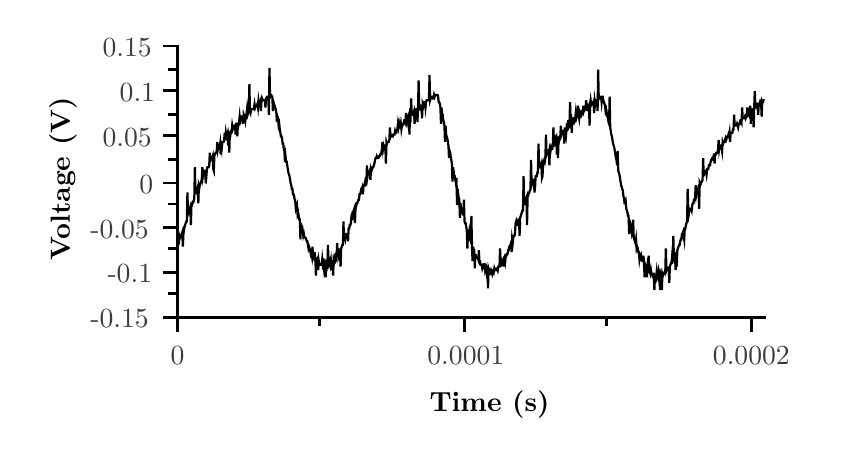
\begin{tikzpicture}{0pt}{0pt}{299pt}{150pt}
	\clip(0pt,150pt) -- (284.325pt,150pt) -- (284.325pt,7.36184pt) -- (0pt,7.36184pt) -- (0pt,150pt);
\begin{scope}
	\clip(54.2025pt,143.344pt) -- (266.258pt,143.344pt) -- (266.258pt,45.3987pt) -- (54.2025pt,45.3987pt) -- (54.2025pt,143.344pt);
	\color[gray]{0}
	\draw[line width=0.8pt, line join=miter, line cap=rect](54.4098pt,71.5173pt) -- (54.6171pt,72.1703pt) -- (54.8244pt,74.7821pt) -- (55.0317pt,74.1292pt) -- (55.2389pt,74.7821pt) -- (55.4462pt,74.7821pt) -- (55.6535pt,75.4351pt) -- (55.8608pt,76.0881pt) -- (56.0681pt,70.8644pt) -- (56.2754pt,75.4351pt) -- (56.4827pt,76.741pt) -- (56.69pt,78.047pt) -- (56.8972pt,78.6999pt) -- (57.1045pt,79.3529pt) -- (57.3118pt,80.0059pt) -- (57.5191pt,80.0059pt) -- (57.7264pt,90.4533pt) -- (57.9337pt,82.6177pt) -- (58.141pt,83.2707pt) -- (58.3483pt,84.5766pt) -- (58.5555pt,84.5766pt) -- (58.7628pt,85.2296pt) -- (58.9701pt,78.6999pt) -- (59.1774pt,85.8826pt) -- (59.3847pt,85.8826pt) -- (59.592pt,86.5355pt) -- (59.7993pt,87.1885pt) -- (60.0066pt,87.1885pt) -- (60.2138pt,88.4944pt) -- (60.4211pt,99.5948pt) -- (60.6284pt,89.8004pt) -- (60.8357pt,91.7593pt) -- (61.043pt,91.7593pt) -- (61.2503pt,91.7593pt) -- (61.4576pt,92.4122pt) -- (61.6649pt,86.5355pt) -- (61.8721pt,93.0652pt) -- (62.0794pt,92.4122pt) -- (62.2867pt,93.7182pt) -- (62.494pt,93.7182pt) -- (62.7013pt,94.3711pt) -- (62.9086pt,95.0241pt) -- (63.1159pt,99.5948pt) -- (63.3232pt,96.33pt) -- (63.5304pt,97.6359pt) -- (63.7377pt,97.6359pt) -- (63.945pt,98.2889pt) -- (64.1523pt,98.2889pt) -- (64.3596pt,93.7182pt) -- (64.5669pt,96.33pt) -- (64.7742pt,98.9419pt) -- (64.9815pt,99.5948pt) -- (65.1888pt,99.5948pt) -- (65.396pt,99.5948pt) -- (65.6033pt,100.248pt) -- (65.8106pt,104.819pt) -- (66.0179pt,102.207pt) -- (66.2252pt,102.86pt) -- (66.4325pt,102.86pt) -- (66.6398pt,102.86pt) -- (66.8471pt,103.513pt) -- (67.0543pt,98.9419pt) -- (67.2616pt,98.2889pt) -- (67.4689pt,104.166pt) -- (67.6762pt,104.166pt) -- (67.8835pt,104.819pt) -- (68.0908pt,104.819pt) -- (68.2981pt,104.819pt) -- (68.5054pt,108.736pt) -- (68.7126pt,106.125pt) -- (68.9199pt,107.43pt) -- (69.1272pt,107.43pt) -- (69.3345pt,106.777pt) -- (69.5418pt,108.083pt) -- (69.7491pt,104.166pt) -- (69.9564pt,108.736pt) -- (70.1637pt,106.777pt) -- (70.3709pt,108.736pt) -- (70.5782pt,108.736pt) -- (70.7855pt,108.736pt) -- (70.9928pt,109.389pt) -- (71.2001pt,112.001pt) -- (71.4074pt,109.389pt) -- (71.6147pt,112.001pt) -- (71.822pt,110.695pt) -- (72.0292pt,111.348pt) -- (72.2365pt,112.001pt) -- (72.4438pt,107.43pt) -- (72.6511pt,112.654pt) -- (72.8584pt,104.819pt) -- (73.0657pt,112.654pt) -- (73.273pt,111.348pt) -- (73.4803pt,112.654pt) -- (73.6876pt,112.654pt) -- (73.8948pt,114.613pt) -- (74.1021pt,113.307pt) -- (74.3094pt,113.96pt) -- (74.5167pt,113.96pt) -- (74.724pt,114.613pt) -- (74.9313pt,114.613pt) -- (75.1386pt,111.348pt) -- (75.3459pt,115.266pt) -- (75.5531pt,115.266pt) -- (75.7604pt,110.695pt) -- (75.9677pt,115.266pt) -- (76.175pt,115.266pt) -- (76.3823pt,115.919pt) -- (76.5896pt,117.878pt) -- (76.7969pt,115.919pt) -- (77.0042pt,116.572pt) -- (77.2114pt,116.572pt) -- (77.4187pt,117.878pt) -- (77.626pt,117.878pt) -- (77.8333pt,115.266pt) -- (78.0406pt,118.531pt) -- (78.2479pt,117.878pt) -- (78.4552pt,117.878pt) -- (78.6625pt,116.572pt) -- (78.8697pt,118.531pt) -- (79.077pt,118.531pt) -- (79.2843pt,120.49pt) -- (79.4916pt,118.531pt) -- (79.6989pt,119.184pt) -- (79.9062pt,119.837pt) -- (80.1135pt,129.631pt) -- (80.3208pt,119.837pt) -- (80.528pt,119.184pt) -- (80.7353pt,120.49pt) -- (80.9426pt,120.49pt) -- (81.1499pt,120.49pt) -- (81.3572pt,120.49pt) -- (81.5645pt,120.49pt) -- (81.7718pt,121.143pt) -- (81.9791pt,122.449pt) -- (82.1863pt,121.143pt) -- (82.3936pt,121.796pt) -- (82.6009pt,121.796pt) -- (82.8082pt,121.796pt) -- (83.0155pt,122.449pt) -- (83.2228pt,121.143pt) -- (83.4301pt,123.755pt) -- (83.6374pt,122.449pt) -- (83.8447pt,122.449pt) -- (84.0519pt,123.102pt) -- (84.2592pt,119.837pt) -- (84.4665pt,123.102pt) -- (84.6738pt,124.408pt) -- (84.8811pt,123.755pt) -- (85.0884pt,123.755pt) -- (85.2957pt,123.755pt) -- (85.503pt,123.755pt) -- (85.7102pt,123.755pt) -- (85.9175pt,121.143pt) -- (86.1248pt,124.408pt) -- (86.3321pt,124.408pt) -- (86.5394pt,125.061pt) -- (86.7467pt,125.061pt) -- (86.954pt,125.061pt) -- (87.1613pt,118.531pt) -- (87.3685pt,135.508pt) -- (87.5758pt,125.061pt) -- (87.7831pt,125.713pt) -- (87.9904pt,125.713pt) -- (88.1977pt,125.061pt) -- (88.405pt,125.061pt) -- (88.6123pt,119.837pt) -- (88.8196pt,123.102pt) -- (89.0268pt,122.449pt) -- (89.2341pt,121.796pt) -- (89.4414pt,121.143pt) -- (89.6487pt,120.49pt) -- (89.856pt,119.184pt) -- (90.0633pt,115.919pt) -- (90.2706pt,117.878pt) -- (90.4779pt,117.225pt) -- (90.6851pt,114.613pt) -- (90.8924pt,115.266pt) -- (91.0997pt,113.307pt) -- (91.307pt,112.001pt) -- (91.5143pt,110.695pt) -- (91.7216pt,110.695pt) -- (91.9289pt,110.042pt) -- (92.1362pt,108.083pt) -- (92.3435pt,108.083pt) -- (92.5507pt,106.125pt) -- (92.758pt,105.472pt) -- (92.9653pt,101.554pt) -- (93.1726pt,103.513pt) -- (93.3799pt,101.554pt) -- (93.5872pt,101.554pt) -- (93.7945pt,100.248pt) -- (94.0018pt,98.9419pt) -- (94.209pt,97.6359pt) -- (94.4163pt,96.983pt) -- (94.6236pt,96.33pt) -- (94.8309pt,95.0241pt) -- (95.0382pt,93.7182pt) -- (95.2455pt,93.0652pt) -- (95.4528pt,91.7593pt) -- (95.6601pt,91.7593pt) -- (95.8673pt,89.8004pt) -- (96.0746pt,89.8004pt) -- (96.2819pt,89.1474pt) -- (96.4892pt,87.8415pt) -- (96.6965pt,87.1885pt) -- (96.9038pt,84.5766pt) -- (97.1111pt,85.2296pt) -- (97.3184pt,85.8826pt) -- (97.5256pt,82.6177pt) -- (97.7329pt,83.2707pt) -- (97.9402pt,81.9648pt) -- (98.1475pt,80.6588pt) -- (98.3548pt,80.6588pt) -- (98.5621pt,73.4762pt) -- (98.7694pt,79.3529pt) -- (98.9767pt,78.047pt) -- (99.1839pt,78.047pt) -- (99.3912pt,76.741pt) -- (99.5985pt,74.7821pt) -- (99.8058pt,75.4351pt) -- (100.013pt,74.1292pt) -- (100.22pt,74.1292pt) -- (100.428pt,74.1292pt) -- (100.635pt,73.4762pt) -- (100.842pt,72.8232pt) -- (101.05pt,72.8232pt) -- (101.257pt,71.5173pt) -- (101.464pt,70.2114pt) -- (101.671pt,70.8644pt) -- (101.879pt,70.2114pt) -- (102.086pt,69.5584pt) -- (102.293pt,68.2525pt) -- (102.501pt,68.9055pt) -- (102.708pt,67.5995pt) -- (102.915pt,70.8644pt) -- (103.122pt,66.9466pt) -- (103.33pt,67.5995pt) -- (103.537pt,66.9466pt) -- (103.744pt,68.9055pt) -- (103.952pt,66.2936pt) -- (104.159pt,60.4169pt) -- (104.366pt,66.9466pt) -- (104.573pt,65.6406pt) -- (104.781pt,66.2936pt) -- (104.988pt,62.3758pt) -- (105.195pt,65.6406pt) -- (105.403pt,64.3347pt) -- (105.61pt,64.3347pt) -- (105.817pt,64.3347pt) -- (106.024pt,64.3347pt) -- (106.232pt,64.3347pt) -- (106.439pt,66.2936pt) -- (106.646pt,64.3347pt) -- (106.854pt,64.9877pt) -- (107.061pt,63.0288pt) -- (107.268pt,64.9877pt) -- (107.475pt,64.3347pt) -- (107.683pt,59.7639pt) -- (107.89pt,64.3347pt) -- (108.097pt,63.6817pt) -- (108.305pt,64.3347pt) -- (108.512pt,71.5173pt) -- (108.719pt,64.3347pt) -- (108.926pt,64.9877pt) -- (109.134pt,65.6406pt) -- (109.341pt,64.3347pt) -- (109.548pt,65.6406pt) -- (109.756pt,62.3758pt) -- (109.963pt,65.6406pt) -- (110.17pt,65.6406pt) -- (110.377pt,60.4169pt) -- (110.585pt,66.2936pt) -- (110.792pt,65.6406pt) -- (110.999pt,66.9466pt) -- (111.207pt,66.2936pt) -- (111.414pt,67.5995pt) -- (111.621pt,66.9466pt) -- (111.829pt,72.1703pt) -- (112.036pt,68.2525pt) -- (112.243pt,68.9055pt) -- (112.45pt,68.9055pt) -- (112.658pt,65.6406pt) -- (112.865pt,70.2114pt) -- (113.072pt,63.6817pt) -- (113.28pt,70.2114pt) -- (113.487pt,70.8644pt) -- (113.694pt,71.5173pt) -- (113.901pt,71.5173pt) -- (114.109pt,80.0059pt) -- (114.316pt,72.8232pt) -- (114.523pt,74.1292pt) -- (114.731pt,73.4762pt) -- (114.938pt,75.4351pt) -- (115.145pt,75.4351pt) -- (115.352pt,75.4351pt) -- (115.56pt,75.4351pt) -- (115.767pt,72.8232pt) -- (115.974pt,77.394pt) -- (116.182pt,77.394pt) -- (116.389pt,78.6999pt) -- (116.596pt,78.6999pt) -- (116.803pt,79.3529pt) -- (117.011pt,81.9648pt) -- (117.218pt,82.6177pt) -- (117.425pt,81.9648pt) -- (117.633pt,83.2707pt) -- (117.84pt,83.9237pt) -- (118.047pt,84.5766pt) -- (118.254pt,79.3529pt) -- (118.462pt,84.5766pt) -- (118.669pt,85.2296pt) -- (118.876pt,86.5355pt) -- (119.084pt,86.5355pt) -- (119.291pt,87.1885pt) -- (119.498pt,87.8415pt) -- (119.705pt,87.8415pt) -- (119.913pt,89.8004pt) -- (120.12pt,89.8004pt) -- (120.327pt,90.4533pt) -- (120.535pt,91.7593pt) -- (120.742pt,91.7593pt) -- (120.949pt,92.4122pt) -- (121.156pt,89.8004pt) -- (121.364pt,93.0652pt) -- (121.571pt,93.0652pt) -- (121.778pt,93.0652pt) -- (121.986pt,94.3711pt) -- (122.193pt,93.7182pt) -- (122.4pt,94.3711pt) -- (122.607pt,100.248pt) -- (122.815pt,96.33pt) -- (123.022pt,97.6359pt) -- (123.229pt,97.6359pt) -- (123.437pt,97.6359pt) -- (123.644pt,98.2889pt) -- (123.851pt,95.0241pt) -- (124.058pt,98.9419pt) -- (124.266pt,98.2889pt) -- (124.473pt,98.9419pt) -- (124.68pt,99.5948pt) -- (124.888pt,99.5948pt) -- (125.095pt,100.248pt) -- (125.302pt,100.901pt) -- (125.509pt,102.207pt) -- (125.717pt,102.86pt) -- (125.924pt,102.86pt) -- (126.131pt,103.513pt) -- (126.339pt,102.86pt) -- (126.546pt,102.86pt) -- (126.753pt,102.86pt) -- (126.961pt,103.513pt) -- (127.168pt,103.513pt) -- (127.375pt,104.166pt) -- (127.582pt,104.166pt) -- (127.79pt,104.819pt) -- (127.997pt,106.125pt) -- (128.204pt,108.736pt) -- (128.412pt,106.125pt) -- (128.619pt,107.43pt) -- (128.826pt,106.777pt) -- (129.033pt,107.43pt) -- (129.241pt,107.43pt) -- (129.448pt,100.901pt) -- (129.655pt,108.736pt) -- (129.863pt,108.083pt) -- (130.07pt,108.736pt) -- (130.277pt,108.736pt) -- (130.484pt,108.736pt) -- (130.692pt,109.389pt) -- (130.899pt,113.96pt) -- (131.106pt,110.695pt) -- (131.314pt,111.348pt) -- (131.521pt,111.348pt) -- (131.728pt,110.695pt) -- (131.935pt,110.695pt) -- (132.143pt,111.348pt) -- (132.35pt,111.348pt) -- (132.557pt,111.348pt) -- (132.765pt,112.654pt) -- (132.972pt,112.001pt) -- (133.179pt,112.001pt) -- (133.386pt,112.654pt) -- (133.594pt,113.307pt) -- (133.801pt,115.266pt) -- (134.008pt,113.96pt) -- (134.216pt,115.266pt) -- (134.423pt,113.96pt) -- (134.63pt,113.96pt) -- (134.837pt,115.266pt) -- (135.045pt,113.307pt) -- (135.252pt,114.613pt) -- (135.459pt,114.613pt) -- (135.667pt,115.266pt) -- (135.874pt,115.266pt) -- (136.081pt,116.572pt) -- (136.288pt,116.572pt) -- (136.496pt,115.919pt) -- (136.703pt,119.184pt) -- (136.91pt,117.225pt) -- (137.118pt,115.919pt) -- (137.325pt,117.225pt) -- (137.532pt,117.878pt) -- (137.739pt,118.531pt) -- (137.947pt,111.348pt) -- (138.154pt,118.531pt) -- (138.361pt,117.878pt) -- (138.569pt,124.408pt) -- (138.776pt,118.531pt) -- (138.983pt,118.531pt) -- (139.19pt,118.531pt) -- (139.398pt,119.184pt) -- (139.605pt,119.837pt) -- (139.812pt,115.266pt) -- (140.02pt,119.837pt) -- (140.227pt,119.837pt) -- (140.434pt,120.49pt) -- (140.642pt,120.49pt) -- (140.849pt,115.919pt) -- (141.056pt,121.143pt) -- (141.263pt,130.937pt) -- (141.471pt,121.143pt) -- (141.678pt,121.796pt) -- (141.885pt,121.143pt) -- (142.093pt,121.796pt) -- (142.3pt,121.796pt) -- (142.507pt,117.225pt) -- (142.714pt,122.449pt) -- (142.922pt,121.796pt) -- (143.129pt,123.102pt) -- (143.336pt,123.102pt) -- (143.544pt,123.102pt) -- (143.751pt,121.143pt) -- (143.958pt,123.102pt) -- (144.165pt,123.755pt) -- (144.373pt,123.755pt) -- (144.58pt,123.755pt) -- (144.787pt,123.755pt) -- (144.995pt,123.755pt) -- (145.202pt,132.896pt) -- (145.409pt,123.755pt) -- (145.616pt,124.408pt) -- (145.824pt,125.061pt) -- (146.031pt,125.061pt) -- (146.238pt,125.061pt) -- (146.446pt,124.408pt) -- (146.653pt,124.408pt) -- (146.86pt,125.713pt) -- (147.067pt,125.061pt) -- (147.275pt,125.713pt) -- (147.482pt,125.713pt) -- (147.689pt,125.713pt) -- (147.897pt,125.713pt) -- (148.104pt,125.713pt) -- (148.311pt,125.061pt) -- (148.518pt,123.102pt) -- (148.726pt,123.102pt) -- (148.933pt,122.449pt) -- (149.14pt,121.143pt) -- (149.348pt,115.266pt) -- (149.555pt,121.143pt) -- (149.762pt,118.531pt) -- (149.969pt,118.531pt) -- (150.177pt,116.572pt) -- (150.384pt,115.919pt) -- (150.591pt,114.613pt) -- (150.799pt,108.736pt) -- (151.006pt,114.613pt) -- (151.213pt,111.348pt) -- (151.42pt,110.695pt) -- (151.628pt,110.042pt) -- (151.835pt,108.736pt) -- (152.042pt,107.43pt) -- (152.25pt,102.86pt) -- (152.457pt,105.472pt) -- (152.664pt,104.819pt) -- (152.871pt,103.513pt) -- (153.079pt,102.207pt) -- (153.286pt,100.901pt) -- (153.493pt,94.3711pt) -- (153.701pt,99.5948pt) -- (153.908pt,98.2889pt) -- (154.115pt,96.33pt) -- (154.322pt,96.33pt) -- (154.53pt,95.0241pt) -- (154.737pt,93.7182pt) -- (154.944pt,95.6771pt) -- (155.152pt,85.8826pt) -- (155.359pt,91.7593pt) -- (155.566pt,89.8004pt) -- (155.774pt,88.4944pt) -- (155.981pt,87.8415pt) -- (156.188pt,81.3118pt) -- (156.395pt,86.5355pt) -- (156.603pt,84.5766pt) -- (156.81pt,84.5766pt) -- (157.017pt,83.2707pt) -- (157.225pt,82.6177pt) -- (157.432pt,82.6177pt) -- (157.639pt,87.8415pt) -- (157.846pt,80.0059pt) -- (158.054pt,79.3529pt) -- (158.261pt,79.3529pt) -- (158.468pt,78.047pt) -- (158.676pt,76.741pt) -- (158.883pt,70.2114pt) -- (159.09pt,75.4351pt) -- (159.297pt,74.7821pt) -- (159.505pt,76.0881pt) -- (159.712pt,73.4762pt) -- (159.919pt,73.4762pt) -- (160.127pt,72.8232pt) -- (160.334pt,81.9648pt) -- (160.541pt,71.5173pt) -- (160.748pt,65.6406pt) -- (160.956pt,70.8644pt) -- (161.163pt,69.5584pt) -- (161.37pt,69.5584pt) -- (161.578pt,63.0288pt) -- (161.785pt,68.2525pt) -- (161.992pt,66.9466pt) -- (162.199pt,66.9466pt) -- (162.407pt,66.9466pt) -- (162.614pt,66.9466pt) -- (162.821pt,66.2936pt) -- (163.029pt,69.5584pt) -- (163.236pt,65.6406pt) -- (163.443pt,65.6406pt) -- (163.65pt,64.3347pt) -- (163.858pt,64.3347pt) -- (164.065pt,64.3347pt) -- (164.272pt,63.0288pt) -- (164.48pt,63.6817pt) -- (164.687pt,63.0288pt) -- (164.894pt,63.0288pt) -- (165.101pt,64.9877pt) -- (165.309pt,62.3758pt) -- (165.516pt,63.0288pt) -- (165.723pt,61.7228pt) -- (165.931pt,63.0288pt) -- (166.138pt,62.3758pt) -- (166.345pt,55.8461pt) -- (166.552pt,63.0288pt) -- (166.76pt,62.3758pt) -- (166.967pt,62.3758pt) -- (167.174pt,61.7228pt) -- (167.382pt,62.3758pt) -- (167.589pt,61.7228pt) -- (167.796pt,61.0699pt) -- (168.003pt,62.3758pt) -- (168.211pt,62.3758pt) -- (168.418pt,61.7228pt) -- (168.625pt,63.0288pt) -- (168.833pt,62.3758pt) -- (169.04pt,62.3758pt) -- (169.247pt,62.3758pt) -- (169.455pt,63.0288pt) -- (169.662pt,63.0288pt) -- (169.869pt,62.3758pt) -- (170.076pt,63.6817pt) -- (170.284pt,63.6817pt) -- (170.491pt,63.6817pt) -- (170.698pt,70.2114pt) -- (170.906pt,63.6817pt) -- (171.113pt,64.9877pt) -- (171.32pt,65.6406pt) -- (171.527pt,64.9877pt) -- (171.735pt,65.6406pt) -- (171.942pt,63.6817pt) -- (172.149pt,66.2936pt) -- (172.357pt,66.9466pt) -- (172.564pt,65.6406pt) -- (172.771pt,67.5995pt) -- (172.978pt,67.5995pt) -- (173.186pt,68.2525pt) -- (173.393pt,68.2525pt) -- (173.6pt,69.5584pt) -- (173.808pt,69.5584pt) -- (174.015pt,70.8644pt) -- (174.222pt,70.8644pt) -- (174.429pt,71.5173pt) -- (174.637pt,72.1703pt) -- (174.844pt,68.9055pt) -- (175.051pt,73.4762pt) -- (175.259pt,72.1703pt) -- (175.466pt,74.1292pt) -- (175.673pt,74.7821pt) -- (175.88pt,74.7821pt) -- (176.088pt,75.4351pt) -- (176.295pt,79.3529pt) -- (176.502pt,80.0059pt) -- (176.71pt,78.6999pt) -- (176.917pt,78.6999pt) -- (177.124pt,79.3529pt) -- (177.331pt,80.6588pt) -- (177.539pt,80.6588pt) -- (177.746pt,74.7821pt) -- (177.953pt,81.3118pt) -- (178.161pt,81.9648pt) -- (178.368pt,82.6177pt) -- (178.575pt,83.2707pt) -- (178.782pt,83.9237pt) -- (178.99pt,83.9237pt) -- (179.197pt,96.33pt) -- (179.404pt,85.8826pt) -- (179.612pt,87.1885pt) -- (179.819pt,87.1885pt) -- (180.026pt,87.8415pt) -- (180.233pt,88.4944pt) -- (180.441pt,78.6999pt) -- (180.648pt,89.1474pt) -- (180.855pt,89.1474pt) -- (181.063pt,90.4533pt) -- (181.27pt,90.4533pt) -- (181.477pt,91.1063pt) -- (181.684pt,91.7593pt) -- (181.892pt,102.207pt) -- (182.099pt,93.0652pt) -- (182.306pt,93.7182pt) -- (182.514pt,94.3711pt) -- (182.721pt,95.0241pt) -- (182.928pt,95.0241pt) -- (183.135pt,90.4533pt) -- (183.343pt,92.4122pt) -- (183.55pt,96.33pt) -- (183.757pt,96.33pt) -- (183.965pt,96.33pt) -- (184.172pt,97.6359pt) -- (184.379pt,97.6359pt) -- (184.587pt,108.083pt) -- (184.794pt,99.5948pt) -- (185.001pt,99.5948pt) -- (185.208pt,100.248pt) -- (185.416pt,100.248pt) -- (185.623pt,100.901pt) -- (185.83pt,95.6771pt) -- (186.038pt,96.33pt) -- (186.245pt,100.901pt) -- (186.452pt,101.554pt) -- (186.659pt,102.207pt) -- (186.867pt,101.554pt) -- (187.074pt,102.86pt) -- (187.281pt,111.348pt) -- (187.489pt,104.166pt) -- (187.696pt,104.819pt) -- (187.903pt,104.819pt) -- (188.11pt,104.819pt) -- (188.318pt,105.472pt) -- (188.525pt,100.248pt) -- (188.732pt,106.125pt) -- (188.94pt,105.472pt) -- (189.147pt,106.777pt) -- (189.354pt,106.125pt) -- (189.561pt,106.125pt) -- (189.769pt,107.43pt) -- (189.976pt,113.96pt) -- (190.183pt,107.43pt) -- (190.391pt,111.348pt) -- (190.598pt,108.736pt) -- (190.805pt,109.389pt) -- (191.012pt,110.042pt) -- (191.22pt,104.166pt) -- (191.427pt,110.042pt) -- (191.634pt,102.86pt) -- (191.842pt,110.695pt) -- (192.049pt,109.389pt) -- (192.256pt,110.695pt) -- (192.463pt,110.695pt) -- (192.671pt,114.613pt) -- (192.878pt,111.348pt) -- (193.085pt,112.001pt) -- (193.293pt,112.001pt) -- (193.5pt,112.654pt) -- (193.707pt,112.654pt) -- (193.914pt,108.083pt) -- (194.122pt,113.96pt) -- (194.329pt,112.654pt) -- (194.536pt,111.348pt) -- (194.744pt,113.96pt) -- (194.951pt,113.307pt) -- (195.158pt,113.96pt) -- (195.365pt,116.572pt) -- (195.573pt,114.613pt) -- (195.78pt,115.266pt) -- (195.987pt,123.102pt) -- (196.195pt,115.919pt) -- (196.402pt,116.572pt) -- (196.609pt,112.001pt) -- (196.816pt,116.572pt) -- (197.024pt,115.919pt) -- (197.231pt,116.572pt) -- (197.438pt,115.919pt) -- (197.646pt,116.572pt) -- (197.853pt,117.225pt) -- (198.06pt,119.184pt) -- (198.268pt,117.225pt) -- (198.475pt,117.878pt) -- (198.682pt,117.878pt) -- (198.889pt,121.796pt) -- (199.097pt,118.531pt) -- (199.304pt,117.225pt) -- (199.511pt,119.184pt) -- (199.719pt,118.531pt) -- (199.926pt,119.184pt) -- (200.133pt,118.531pt) -- (200.34pt,119.184pt) -- (200.548pt,119.184pt) -- (200.755pt,121.796pt) -- (200.962pt,119.837pt) -- (201.17pt,120.49pt) -- (201.377pt,120.49pt) -- (201.584pt,120.49pt) -- (201.791pt,123.755pt) -- (201.999pt,119.837pt) -- (202.206pt,121.796pt) -- (202.413pt,121.143pt) -- (202.621pt,121.143pt) -- (202.828pt,121.796pt) -- (203.035pt,114.613pt) -- (203.242pt,121.796pt) -- (203.45pt,123.755pt) -- (203.657pt,122.449pt) -- (203.864pt,123.102pt) -- (204.072pt,123.102pt) -- (204.279pt,122.449pt) -- (204.486pt,123.102pt) -- (204.693pt,119.184pt) -- (204.901pt,123.755pt) -- (205.108pt,122.449pt) -- (205.315pt,123.755pt) -- (205.523pt,123.755pt) -- (205.73pt,123.755pt) -- (205.937pt,119.837pt) -- (206.144pt,134.855pt) -- (206.352pt,124.408pt) -- (206.559pt,125.061pt) -- (206.766pt,125.061pt) -- (206.974pt,125.061pt) -- (207.181pt,125.061pt) -- (207.388pt,123.102pt) -- (207.595pt,125.061pt) -- (207.803pt,125.061pt) -- (208.01pt,123.755pt) -- (208.217pt,123.102pt) -- (208.425pt,122.449pt) -- (208.632pt,121.796pt) -- (208.839pt,119.837pt) -- (209.046pt,120.49pt) -- (209.254pt,119.184pt) -- (209.461pt,117.878pt) -- (209.668pt,117.878pt) -- (209.876pt,115.919pt) -- (210.083pt,115.266pt) -- (210.29pt,125.061pt) -- (210.497pt,113.96pt) -- (210.705pt,112.654pt) -- (210.912pt,111.348pt) -- (211.119pt,110.695pt) -- (211.327pt,109.389pt) -- (211.534pt,108.083pt) -- (211.741pt,107.43pt) -- (211.948pt,106.777pt) -- (212.156pt,105.472pt) -- (212.363pt,104.166pt) -- (212.57pt,102.86pt) -- (212.778pt,102.207pt) -- (212.985pt,100.248pt) -- (213.192pt,105.472pt) -- (213.4pt,98.2889pt) -- (213.607pt,97.6359pt) -- (213.814pt,96.983pt) -- (214.021pt,95.6771pt) -- (214.229pt,94.3711pt) -- (214.436pt,93.0652pt) -- (214.643pt,92.4122pt) -- (214.851pt,91.7593pt) -- (215.058pt,91.1063pt) -- (215.265pt,89.1474pt) -- (215.472pt,88.4944pt) -- (215.68pt,86.5355pt) -- (215.887pt,86.5355pt) -- (216.094pt,87.1885pt) -- (216.302pt,84.5766pt) -- (216.509pt,83.9237pt) -- (216.716pt,83.2707pt) -- (216.923pt,81.9648pt) -- (217.131pt,81.9648pt) -- (217.338pt,75.4351pt) -- (217.545pt,80.0059pt) -- (217.753pt,79.3529pt) -- (217.96pt,78.047pt) -- (218.167pt,77.394pt) -- (218.374pt,75.4351pt) -- (218.582pt,76.0881pt) -- (218.789pt,80.6588pt) -- (218.996pt,74.1292pt) -- (219.204pt,73.4762pt) -- (219.411pt,72.8232pt) -- (219.618pt,72.1703pt) -- (219.825pt,73.4762pt) -- (220.033pt,70.2114pt) -- (220.24pt,70.8644pt) -- (220.447pt,70.2114pt) -- (220.655pt,68.9055pt) -- (220.862pt,68.9055pt) -- (221.069pt,66.2936pt) -- (221.276pt,67.5995pt) -- (221.484pt,66.9466pt) -- (221.691pt,67.5995pt) -- (221.898pt,66.2936pt) -- (222.106pt,65.6406pt) -- (222.313pt,65.6406pt) -- (222.52pt,67.5995pt) -- (222.727pt,64.3347pt) -- (222.935pt,59.7639pt) -- (223.142pt,64.3347pt) -- (223.349pt,63.6817pt) -- (223.557pt,63.0288pt) -- (223.764pt,59.7639pt) -- (223.971pt,63.0288pt) -- (224.178pt,61.7228pt) -- (224.386pt,67.5995pt) -- (224.593pt,61.7228pt) -- (224.8pt,61.7228pt) -- (225.008pt,61.0699pt) -- (225.215pt,62.3758pt) -- (225.422pt,61.0699pt) -- (225.629pt,61.0699pt) -- (225.837pt,60.4169pt) -- (226.044pt,61.0699pt) -- (226.251pt,61.0699pt) -- (226.459pt,55.1932pt) -- (226.666pt,60.4169pt) -- (226.873pt,60.4169pt) -- (227.081pt,59.7639pt) -- (227.288pt,61.7228pt) -- (227.495pt,59.7639pt) -- (227.702pt,60.4169pt) -- (227.91pt,61.7228pt) -- (228.117pt,59.7639pt) -- (228.324pt,61.0699pt) -- (228.532pt,55.1932pt) -- (228.739pt,61.0699pt) -- (228.946pt,60.4169pt) -- (229.153pt,55.1932pt) -- (229.361pt,61.0699pt) -- (229.568pt,60.4169pt) -- (229.775pt,61.0699pt) -- (229.983pt,61.0699pt) -- (230.19pt,61.7228pt) -- (230.397pt,61.7228pt) -- (230.604pt,70.2114pt) -- (230.812pt,62.3758pt) -- (231.019pt,63.0288pt) -- (231.226pt,62.3758pt) -- (231.434pt,62.3758pt) -- (231.641pt,63.6817pt) -- (231.848pt,57.805pt) -- (232.055pt,63.6817pt) -- (232.263pt,64.3347pt) -- (232.47pt,64.9877pt) -- (232.677pt,64.9877pt) -- (232.885pt,67.5995pt) -- (233.092pt,66.2936pt) -- (233.299pt,74.7821pt) -- (233.506pt,66.9466pt) -- (233.714pt,67.5995pt) -- (233.921pt,67.5995pt) -- (234.128pt,62.3758pt) -- (234.336pt,68.9055pt) -- (234.543pt,63.6817pt) -- (234.75pt,69.5584pt) -- (234.957pt,70.2114pt) -- (235.165pt,70.8644pt) -- (235.372pt,71.5173pt) -- (235.579pt,71.5173pt) -- (235.787pt,72.8232pt) -- (235.994pt,73.4762pt) -- (236.201pt,73.4762pt) -- (236.408pt,75.4351pt) -- (236.616pt,75.4351pt) -- (236.823pt,76.0881pt) -- (237.03pt,74.7821pt) -- (237.238pt,73.4762pt) -- (237.445pt,77.394pt) -- (237.652pt,77.394pt) -- (237.859pt,78.6999pt) -- (238.067pt,79.3529pt) -- (238.274pt,80.0059pt) -- (238.481pt,91.7593pt) -- (238.689pt,84.5766pt) -- (238.896pt,82.6177pt) -- (239.103pt,83.9237pt) -- (239.31pt,84.5766pt) -- (239.518pt,84.5766pt) -- (239.725pt,84.5766pt) -- (239.932pt,83.9237pt) -- (240.14pt,85.8826pt) -- (240.347pt,86.5355pt) -- (240.554pt,86.5355pt) -- (240.761pt,87.8415pt) -- (240.969pt,87.8415pt) -- (241.176pt,88.4944pt) -- (241.383pt,93.0652pt) -- (241.591pt,89.8004pt) -- (241.798pt,91.1063pt) -- (242.005pt,91.7593pt) -- (242.213pt,91.7593pt) -- (242.42pt,92.4122pt) -- (242.627pt,84.5766pt) -- (242.834pt,93.7182pt) -- (243.042pt,93.0652pt) -- (243.249pt,93.7182pt) -- (243.456pt,94.3711pt) -- (243.664pt,94.3711pt) -- (243.871pt,95.0241pt) -- (244.078pt,102.86pt) -- (244.285pt,96.33pt) -- (244.493pt,97.6359pt) -- (244.7pt,97.6359pt) -- (244.907pt,98.2889pt) -- (245.115pt,98.2889pt) -- (245.322pt,96.983pt) -- (245.529pt,98.9419pt) -- (245.736pt,98.9419pt) -- (245.944pt,98.9419pt) -- (246.151pt,100.248pt) -- (246.358pt,100.248pt) -- (246.566pt,100.248pt) -- (246.773pt,101.554pt) -- (246.98pt,102.207pt) -- (247.187pt,102.207pt) -- (247.395pt,102.86pt) -- (247.602pt,102.86pt) -- (247.809pt,103.513pt) -- (248.017pt,102.86pt) -- (248.224pt,100.901pt) -- (248.431pt,104.166pt) -- (248.638pt,104.166pt) -- (248.846pt,104.819pt) -- (249.053pt,104.819pt) -- (249.26pt,104.819pt) -- (249.468pt,106.125pt) -- (249.675pt,109.389pt) -- (249.882pt,106.125pt) -- (250.089pt,107.43pt) -- (250.297pt,107.43pt) -- (250.504pt,107.43pt) -- (250.711pt,106.777pt) -- (250.919pt,105.472pt) -- (251.126pt,108.736pt) -- (251.333pt,108.083pt) -- (251.54pt,108.736pt) -- (251.748pt,108.736pt) -- (251.955pt,109.389pt) -- (252.162pt,110.042pt) -- (252.37pt,109.389pt) -- (252.577pt,110.042pt) -- (252.784pt,110.695pt) -- (252.991pt,110.695pt) -- (253.199pt,111.348pt) -- (253.406pt,110.695pt) -- (253.613pt,112.001pt) -- (253.821pt,108.736pt) -- (254.028pt,112.001pt) -- (254.235pt,112.001pt) -- (254.442pt,112.001pt) -- (254.65pt,112.001pt) -- (254.857pt,113.307pt) -- (255.064pt,113.307pt) -- (255.272pt,118.531pt) -- (255.479pt,114.613pt) -- (255.686pt,114.613pt) -- (255.894pt,114.613pt) -- (256.101pt,114.613pt) -- (256.308pt,115.266pt) -- (256.515pt,114.613pt) -- (256.723pt,113.96pt) -- (256.93pt,115.266pt) -- (257.137pt,115.266pt) -- (257.345pt,115.266pt) -- (257.552pt,116.572pt) -- (257.759pt,116.572pt) -- (257.966pt,115.919pt) -- (258.174pt,121.143pt) -- (258.381pt,117.225pt) -- (258.588pt,117.225pt) -- (258.796pt,117.225pt) -- (259.003pt,117.225pt) -- (259.21pt,117.878pt) -- (259.417pt,117.225pt) -- (259.625pt,117.878pt) -- (259.832pt,117.878pt) -- (260.039pt,121.143pt) -- (260.247pt,119.184pt) -- (260.454pt,119.184pt) -- (260.661pt,118.531pt) -- (260.868pt,119.184pt) -- (261.076pt,121.796pt) -- (261.283pt,115.266pt) -- (261.49pt,119.837pt) -- (261.698pt,120.49pt) -- (261.905pt,120.49pt) -- (262.112pt,120.49pt) -- (262.319pt,113.96pt) -- (262.527pt,121.143pt) -- (262.734pt,127.019pt) -- (262.941pt,121.796pt) -- (263.149pt,121.143pt) -- (263.356pt,121.143pt) -- (263.563pt,121.796pt) -- (263.77pt,121.143pt) -- (263.978pt,118.531pt) -- (264.185pt,122.449pt) -- (264.392pt,122.449pt) -- (264.6pt,123.102pt) -- (264.807pt,122.449pt) -- (265.014pt,123.102pt) -- (265.221pt,117.878pt) -- (265.429pt,123.102pt) -- (265.636pt,123.102pt) -- (265.843pt,123.755pt) -- (266.051pt,123.755pt) -- (266.258pt,123.755pt);
\end{scope}
\begin{scope}
	\color[gray]{0}
	\pgftext[center, base, at={\pgfpoint{15.2147pt}{95.3146pt}},rotate=90]{\textbf{Voltage (V)}}
	\color[gray]{0.235294}
	\pgftext[center, base, at={\pgfpoint{33.2154pt}{41.595pt}}]{-0.15}
	\pgftext[center, base, at={\pgfpoint{36.9076pt}{57.7607pt}}]{-0.1}
	\pgftext[center, base, at={\pgfpoint{33.2154pt}{73.9263pt}}]{-0.05}
	\pgftext[center, base, at={\pgfpoint{42.9029pt}{90.092pt}}]{0}
	\pgftext[center, base, at={\pgfpoint{35.9567pt}{107.209pt}}]{0.05}
	\pgftext[center, base, at={\pgfpoint{39.649pt}{123.374pt}}]{0.1}
	\pgftext[center, base, at={\pgfpoint{35.9567pt}{139.54pt}}]{0.15}
	\color[gray]{0}
	\draw[line width=1pt, line join=bevel, line cap=rect](54.2025pt,53.957pt) -- (51.3497pt,53.957pt);
	\draw[line width=1pt, line join=bevel, line cap=rect](54.2025pt,70.1226pt) -- (51.3497pt,70.1226pt);
	\draw[line width=1pt, line join=bevel, line cap=rect](54.2025pt,86.2883pt) -- (51.3497pt,86.2883pt);
	\draw[line width=1pt, line join=bevel, line cap=rect](54.2025pt,102.454pt) -- (51.3497pt,102.454pt);
	\draw[line width=1pt, line join=bevel, line cap=rect](54.2025pt,118.62pt) -- (51.3497pt,118.62pt);
	\draw[line width=1pt, line join=bevel, line cap=rect](54.2025pt,134.785pt) -- (51.3497pt,134.785pt);
	\draw[line width=1pt, line join=bevel, line cap=rect](54.2025pt,45.3987pt) -- (49.4479pt,45.3987pt);
	\draw[line width=1pt, line join=bevel, line cap=rect](54.2025pt,61.5643pt) -- (49.4479pt,61.5643pt);
	\draw[line width=1pt, line join=bevel, line cap=rect](54.2025pt,77.73pt) -- (49.4479pt,77.73pt);
	\draw[line width=1pt, line join=bevel, line cap=rect](54.2025pt,93.8957pt) -- (49.4479pt,93.8957pt);
	\draw[line width=1pt, line join=bevel, line cap=rect](54.2025pt,111.012pt) -- (49.4479pt,111.012pt);
	\draw[line width=1pt, line join=bevel, line cap=rect](54.2025pt,127.178pt) -- (49.4479pt,127.178pt);
	\draw[line width=1pt, line join=bevel, line cap=rect](54.2025pt,143.344pt) -- (49.4479pt,143.344pt);
	\draw[line width=1pt, line join=bevel, line cap=rect](54.2025pt,143.344pt) -- (54.2025pt,45.3987pt);
	\pgftext[center, base, at={\pgfpoint{166.887pt}{11.1655pt}}]{\textbf{Time (s)}}
	\color[gray]{0.235294}
	\pgftext[center, base, at={\pgfpoint{54.1951pt}{28.2821pt}}]{0}
	\pgftext[center, base, at={\pgfpoint{158.328pt}{28.2821pt}}]{0.0001}
	\pgftext[center, base, at={\pgfpoint{261.503pt}{28.2821pt}}]{0.0002}
	\color[gray]{0}
	\draw[line width=1pt, line join=bevel, line cap=rect](105.552pt,45.3987pt) -- (105.552pt,42.5459pt);
	\draw[line width=1pt, line join=bevel, line cap=rect](209.203pt,45.3987pt) -- (209.203pt,42.5459pt);
	\draw[line width=1pt, line join=bevel, line cap=rect](54.2025pt,45.3987pt) -- (54.2025pt,40.6441pt);
	\draw[line width=1pt, line join=bevel, line cap=rect](157.853pt,45.3987pt) -- (157.853pt,40.6441pt);
	\draw[line width=1pt, line join=bevel, line cap=rect](261.503pt,45.3987pt) -- (261.503pt,40.6441pt);
	\draw[line width=1pt, line join=bevel, line cap=rect](54.2025pt,45.3987pt) -- (266.258pt,45.3987pt);
\end{scope}
\end{tikzpicture}

		\caption{New signal produced when the two 7555 chips are used in the circuit and combined by the mixer.}
		\label{fig:7555}
\end{figure}

\subsection{Mixer - SA612A}
\label{sec:SA612A-mixer}
The mixer chip is used to calculate the difference in frequency between the input signals and output this difference as a new signal. This allows a small influence to the circuit to cause a big difference in the signal by comparing two high frequency inputs so that the relative difference is large. The chip that is used is the SA612A IC which is a double-balanced mixer and oscillator\cite{SA612A}. The pin configuration and internal block configuration is shown in appendix~\ref{app:SA612A}. This particular mixer chip subtracts the lower frequency signal from the higher one to give a simple difference relation.

The chip is tested using a pair of TG315 signal generators to provide a known input frequency that can be used to examine the performance of the mixer chip. It is found, when using this set-up, that though the output signal is the difference between the inputs, as expected, the signal is not perfectly clean, and there is a considerable amount of high frequency noise left. This produces a unpleasant rough high pitched addition to the sound. This is required to be removed in order that the instrument be acceptable to listen to. These unwanted parts of the signal shall be removed using a low pass filter.

\subsection{Low Pass Filter}
\label{sec:lowpass}
A low pass filter is a circuit whose output depends on the frequency of the input. The circuit has a cut off frequency, above which the amplitude of the signal is severely attenuated. This cut-off can be chosen depending on the components used. This allows the high frequency noise to be removed whilst leaving the important signal largely unaffected.

The low pass filter is composed of a resistor and a capacitor to ground, as shown in figure~\ref{fig:low_pass}. The capacitor acts as an open circuit at low frequency signals, so these parts are not affected, but acts as a short circuit at high frequencies, so these pass to ground and hence are removed from signal. To satisfactorily remove the noise, two low pass filters are placed in series with a $\times 1$ buffer amplifier between them. This produces a sharper cut-off so that less of the important signal is lost. The buffer amplifier is added to ensure the two filters are isolated from each other. It is formed of an operational-amplifier (op-amp) with the output fed back into the inverting input. The op-amp used is the LT081 operational amplifier, described in appendix~\ref{app:lt081}.

\begin{figure}[htbp]
	\begin{center}
		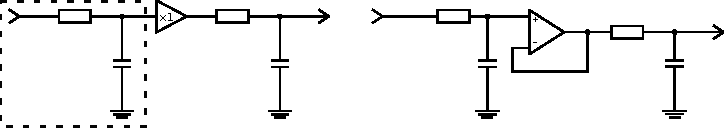
\includegraphics[width=\textwidth]{report_img/buffer_amp}
		\caption{The low pass filter is an extremely simple circuit to remove unwanted high frequency noise. The circuit on the left shows the principle of having two low pass filters separated by a $\times 1$ buffer amplifier, with the single low pass filter highlighted. The second circuit shows the implementation of the op-amp bases buffer.}
		\label{fig:low_pass}
	\end{center}
\end{figure}

The approximate frequency of the cut-off of the low pass filter is given by the equation
\begin{equation}
	f_c = \frac{1}{2\pi RC},
\end{equation}
where $R$ is the resistor and $C$ is the capacitor in the previous circuit. A cut-off of around 20\,kHz is desired, corresponding to the upper limit of human hearing, and so a resistor of 820\,$\Omega$ and capacitor of 10\,nF is used. Equation~\ref{eqn:low pass numbers} shows that this gives a value that is very close to the desired value,
\begin{equation}
		f_c \frac{1}{2\pi\times 820 \times 10 \times 10^{-9}} = 19,409\,\text{Hz}.
		\label{eqn:low pass numbers}
\end{equation}
The resulting signal is much cleaner in the high frequency range and so much more pleasant to listen to. A comparison of the signal before and after the low pass filter is shown in figure~\ref{fig:filter before after}.

\begin{figure}[htbp]
	\centering
		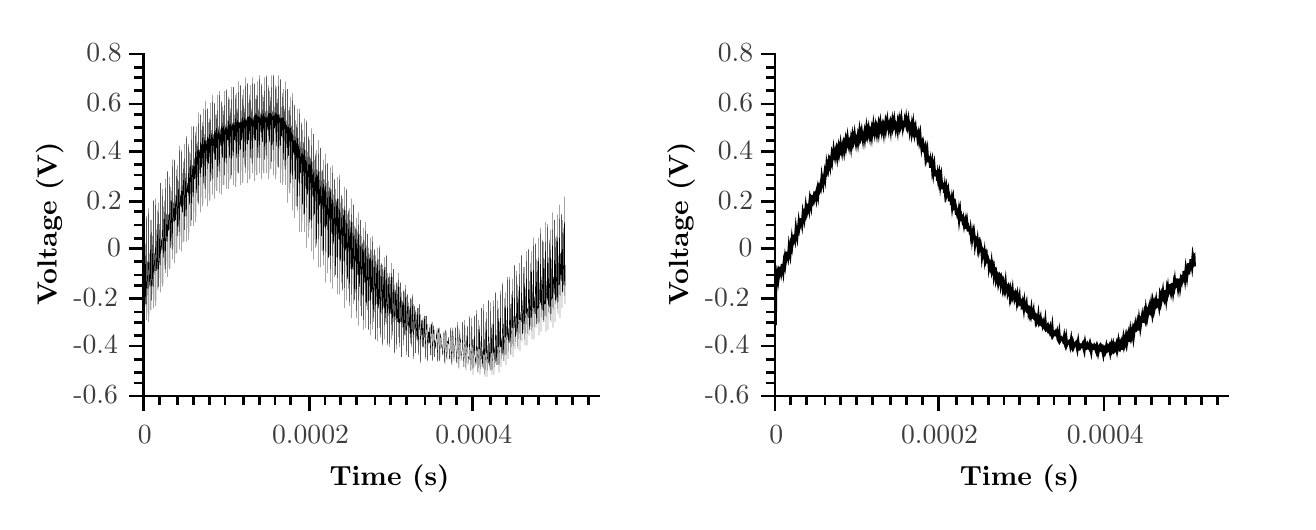
\begin{tikzpicture}{0pt}{0pt}{479pt}{180pt}
	\clip(0pt,180pt) -- (455.491pt,180pt) -- (455.491pt,8.83421pt) -- (0pt,8.83421pt) -- (0pt,180pt);
\begin{scope}
	\clip(270.062pt,170.491pt) -- (433.62pt,170.491pt) -- (433.62pt,46.8711pt) -- (270.062pt,46.8711pt) -- (270.062pt,170.491pt);
	\color[gray]{0}
	\draw[line width=1pt, line join=miter, line cap=rect](270.21pt,73.0078pt) -- (270.358pt,85.0166pt) -- (270.506pt,87.4183pt) -- (270.654pt,88.8311pt) -- (270.802pt,90.5265pt) -- (270.95pt,89.6788pt) -- (271.099pt,90.6678pt) -- (271.247pt,89.3962pt) -- (271.395pt,90.5265pt) -- (271.543pt,91.0916pt) -- (271.691pt,90.9503pt) -- (271.839pt,93.6346pt) -- (271.988pt,92.0806pt) -- (272.136pt,92.2218pt) -- (272.284pt,91.3742pt) -- (272.432pt,92.2218pt) -- (272.58pt,94.6236pt) -- (272.728pt,93.3521pt) -- (272.876pt,93.4934pt) -- (273.025pt,92.3631pt) -- (273.173pt,94.0585pt) -- (273.321pt,95.4713pt) -- (273.469pt,94.9062pt) -- (273.617pt,96.1777pt) -- (273.765pt,94.9062pt) -- (273.913pt,96.0364pt) -- (274.062pt,96.1777pt) -- (274.21pt,96.3189pt) -- (274.358pt,99.0033pt) -- (274.506pt,97.7317pt) -- (274.654pt,98.0143pt) -- (274.802pt,97.1666pt) -- (274.951pt,98.2969pt) -- (275.099pt,100.275pt) -- (275.247pt,99.1445pt) -- (275.395pt,99.5684pt) -- (275.543pt,98.5794pt) -- (275.691pt,100.416pt) -- (275.839pt,101.829pt) -- (275.988pt,101.405pt) -- (276.136pt,102.959pt) -- (276.284pt,101.688pt) -- (276.432pt,102.818pt) -- (276.58pt,102.394pt) -- (276.728pt,102.818pt) -- (276.877pt,105.22pt) -- (277.025pt,104.089pt) -- (277.173pt,104.513pt) -- (277.321pt,103.665pt) -- (277.469pt,104.937pt) -- (277.617pt,106.915pt) -- (277.765pt,105.785pt) -- (277.914pt,106.209pt) -- (278.062pt,105.22pt) -- (278.21pt,107.197pt) -- (278.358pt,107.763pt) -- (278.506pt,107.48pt) -- (278.654pt,109.175pt) -- (278.802pt,108.045pt) -- (278.951pt,109.034pt) -- (279.099pt,108.61pt) -- (279.247pt,109.175pt) -- (279.395pt,111.153pt) -- (279.543pt,109.882pt) -- (279.691pt,110.164pt) -- (279.84pt,109.175pt) -- (279.988pt,110.588pt) -- (280.136pt,112.566pt) -- (280.284pt,111.718pt) -- (280.432pt,112.284pt) -- (280.58pt,111.436pt) -- (280.728pt,113.414pt) -- (280.877pt,113.414pt) -- (281.025pt,113.131pt) -- (281.173pt,114.685pt) -- (281.321pt,113.414pt) -- (281.469pt,114.261pt) -- (281.617pt,113.555pt) -- (281.765pt,114.261pt) -- (281.914pt,116.381pt) -- (282.062pt,115.25pt) -- (282.21pt,115.392pt) -- (282.358pt,114.544pt) -- (282.506pt,116.098pt) -- (282.654pt,117.511pt) -- (282.803pt,116.522pt) -- (282.951pt,117.228pt) -- (283.099pt,116.239pt) -- (283.247pt,118.076pt) -- (283.395pt,117.793pt) -- (283.543pt,117.652pt) -- (283.691pt,119.489pt) -- (283.84pt,118.217pt) -- (283.988pt,118.782pt) -- (284.136pt,117.935pt) -- (284.284pt,118.641pt) -- (284.432pt,120.76pt) -- (284.58pt,119.489pt) -- (284.729pt,119.63pt) -- (284.877pt,118.782pt) -- (285.025pt,120.619pt) -- (285.173pt,121.184pt) -- (285.321pt,120.336pt) -- (285.469pt,121.325pt) -- (285.617pt,120.195pt) -- (285.766pt,121.891pt) -- (285.914pt,121.325pt) -- (286.062pt,121.467pt) -- (286.21pt,123.727pt) -- (286.358pt,122.597pt) -- (286.506pt,123.303pt) -- (286.654pt,122.597pt) -- (286.803pt,123.586pt) -- (286.951pt,125.423pt) -- (287.099pt,124.292pt) -- (287.247pt,124.857pt) -- (287.395pt,124.01pt) -- (287.543pt,126.129pt) -- (287.692pt,126.129pt) -- (287.84pt,125.705pt) -- (287.988pt,126.977pt) -- (288.136pt,125.988pt) -- (288.284pt,127.824pt) -- (288.432pt,127.4pt) -- (288.58pt,127.683pt) -- (288.729pt,129.944pt) -- (288.877pt,128.955pt) -- (289.025pt,129.802pt) -- (289.173pt,129.096pt) -- (289.321pt,130.509pt) -- (289.469pt,131.498pt) -- (289.617pt,130.65pt) -- (289.766pt,131.356pt) -- (289.914pt,130.509pt) -- (290.062pt,132.628pt) -- (290.21pt,132.487pt) -- (290.358pt,131.921pt) -- (290.506pt,133.334pt) -- (290.655pt,132.345pt) -- (290.803pt,133.899pt) -- (290.951pt,133.334pt) -- (291.099pt,133.758pt) -- (291.247pt,135.312pt) -- (291.395pt,134.182pt) -- (291.543pt,134.606pt) -- (291.692pt,133.758pt) -- (291.84pt,135.03pt) -- (291.988pt,135.595pt) -- (292.136pt,134.464pt) -- (292.284pt,134.888pt) -- (292.432pt,133.899pt) -- (292.58pt,135.877pt) -- (292.729pt,135.312pt) -- (292.877pt,134.747pt) -- (293.025pt,136.019pt) -- (293.173pt,134.888pt) -- (293.321pt,136.019pt) -- (293.469pt,135.312pt) -- (293.618pt,135.736pt) -- (293.766pt,137.149pt) -- (293.914pt,135.877pt) -- (294.062pt,136.301pt) -- (294.21pt,135.453pt) -- (294.358pt,137.008pt) -- (294.506pt,137.573pt) -- (294.655pt,136.584pt) -- (294.803pt,137.008pt) -- (294.951pt,136.019pt) -- (295.099pt,137.855pt) -- (295.247pt,137.29pt) -- (295.395pt,137.008pt) -- (295.544pt,138.42pt) -- (295.692pt,137.29pt) -- (295.84pt,138.42pt) -- (295.988pt,137.573pt) -- (296.136pt,138.138pt) -- (296.284pt,139.551pt) -- (296.432pt,138.279pt) -- (296.581pt,138.562pt) -- (296.729pt,137.714pt) -- (296.877pt,139.127pt) -- (297.025pt,139.409pt) -- (297.173pt,138.279pt) -- (297.321pt,138.703pt) -- (297.469pt,137.573pt) -- (297.618pt,139.409pt) -- (297.766pt,138.703pt) -- (297.914pt,138.562pt) -- (298.062pt,140.116pt) -- (298.21pt,138.985pt) -- (298.358pt,139.974pt) -- (298.507pt,139.268pt) -- (298.655pt,139.974pt) -- (298.803pt,141.105pt) -- (298.951pt,139.833pt) -- (299.099pt,139.974pt) -- (299.247pt,138.985pt) -- (299.395pt,140.539pt) -- (299.544pt,140.681pt) -- (299.692pt,139.692pt) -- (299.84pt,140.398pt) -- (299.988pt,139.268pt) -- (300.136pt,140.963pt) -- (300.284pt,140.398pt) -- (300.432pt,140.398pt) -- (300.581pt,141.952pt) -- (300.729pt,140.681pt) -- (300.877pt,141.528pt) -- (301.025pt,140.681pt) -- (301.173pt,141.387pt) -- (301.321pt,142.235pt) -- (301.47pt,140.963pt) -- (301.618pt,141.105pt) -- (301.766pt,140.116pt) -- (301.914pt,141.811pt) -- (302.062pt,141.811pt) -- (302.21pt,141.105pt) -- (302.358pt,141.952pt) -- (302.507pt,140.681pt) -- (302.655pt,142.235pt) -- (302.803pt,141.67pt) -- (302.951pt,141.528pt) -- (303.099pt,143.083pt) -- (303.247pt,141.811pt) -- (303.395pt,142.517pt) -- (303.544pt,141.528pt) -- (303.692pt,142.517pt) -- (303.84pt,143.365pt) -- (303.988pt,142.235pt) -- (304.136pt,142.376pt) -- (304.284pt,141.387pt) -- (304.433pt,143.083pt) -- (304.581pt,142.8pt) -- (304.729pt,141.952pt) -- (304.877pt,142.8pt) -- (305.025pt,141.528pt) -- (305.173pt,143.083pt) -- (305.321pt,142.376pt) -- (305.47pt,142.517pt) -- (305.618pt,144.071pt) -- (305.766pt,142.8pt) -- (305.914pt,143.224pt) -- (306.062pt,142.235pt) -- (306.21pt,143.365pt) -- (306.359pt,144.213pt) -- (306.507pt,143.083pt) -- (306.655pt,143.365pt) -- (306.803pt,142.376pt) -- (306.951pt,144.071pt) -- (307.099pt,143.648pt) -- (307.247pt,142.941pt) -- (307.396pt,144.071pt) -- (307.544pt,142.8pt) -- (307.692pt,144.213pt) -- (307.84pt,143.365pt) -- (307.988pt,143.648pt) -- (308.136pt,144.919pt) -- (308.284pt,143.648pt) -- (308.433pt,144.071pt) -- (308.581pt,143.083pt) -- (308.729pt,144.213pt) -- (308.877pt,144.778pt) -- (309.025pt,143.648pt) -- (309.173pt,143.789pt) -- (309.322pt,142.659pt) -- (309.47pt,144.495pt) -- (309.618pt,144.071pt) -- (309.766pt,143.506pt) -- (309.914pt,144.778pt) -- (310.062pt,143.648pt) -- (310.21pt,144.919pt) -- (310.359pt,144.071pt) -- (310.507pt,144.495pt) -- (310.655pt,145.767pt) -- (310.803pt,144.495pt) -- (310.951pt,144.778pt) -- (311.099pt,143.789pt) -- (311.247pt,145.06pt) -- (311.396pt,145.484pt) -- (311.544pt,144.354pt) -- (311.692pt,144.637pt) -- (311.84pt,143.506pt) -- (311.988pt,145.343pt) -- (312.136pt,144.778pt) -- (312.285pt,144.354pt) -- (312.433pt,145.626pt) -- (312.581pt,144.354pt) -- (312.729pt,145.202pt) -- (312.877pt,144.213pt) -- (313.025pt,144.637pt) -- (313.173pt,145.908pt) -- (313.322pt,144.637pt) -- (313.47pt,144.919pt) -- (313.618pt,143.93pt) -- (313.766pt,145.202pt) -- (313.914pt,145.343pt) -- (314.062pt,144.354pt) -- (314.211pt,144.778pt) -- (314.359pt,143.648pt) -- (314.507pt,145.484pt) -- (314.655pt,144.778pt) -- (314.803pt,144.354pt) -- (314.951pt,145.767pt) -- (315.099pt,144.637pt) -- (315.248pt,145.626pt) -- (315.396pt,144.778pt) -- (315.544pt,145.484pt) -- (315.692pt,146.615pt) -- (315.84pt,145.202pt) -- (315.988pt,145.343pt) -- (316.136pt,144.354pt) -- (316.285pt,145.767pt) -- (316.433pt,145.767pt) -- (316.581pt,144.778pt) -- (316.729pt,145.343pt) -- (316.877pt,144.071pt) -- (317.025pt,145.908pt) -- (317.174pt,145.202pt) -- (317.322pt,144.919pt) -- (317.47pt,146.332pt) -- (317.618pt,145.06pt) -- (317.766pt,145.626pt) -- (317.914pt,144.637pt) -- (318.062pt,145.484pt) -- (318.211pt,146.332pt) -- (318.359pt,144.778pt) -- (318.507pt,144.919pt) -- (318.655pt,143.648pt) -- (318.803pt,145.202pt) -- (318.951pt,144.919pt) -- (319.099pt,143.789pt) -- (319.248pt,144.354pt) -- (319.396pt,142.941pt) -- (319.544pt,144.354pt) -- (319.692pt,143.365pt) -- (319.84pt,143.224pt) -- (319.988pt,144.495pt) -- (320.137pt,142.8pt) -- (320.285pt,143.365pt) -- (320.433pt,142.235pt) -- (320.581pt,143.365pt) -- (320.729pt,143.93pt) -- (320.877pt,142.094pt) -- (321.025pt,141.952pt) -- (321.174pt,140.398pt) -- (321.322pt,141.952pt) -- (321.47pt,141.387pt) -- (321.618pt,140.116pt) -- (321.766pt,140.822pt) -- (321.914pt,138.985pt) -- (322.062pt,140.257pt) -- (322.211pt,138.985pt) -- (322.359pt,139.692pt) -- (322.507pt,140.681pt) -- (322.655pt,138.703pt) -- (322.803pt,138.844pt) -- (322.951pt,137.431pt) -- (323.1pt,138.703pt) -- (323.248pt,138.985pt) -- (323.396pt,137.008pt) -- (323.544pt,136.866pt) -- (323.692pt,135.03pt) -- (323.84pt,136.584pt) -- (323.988pt,135.736pt) -- (324.137pt,135.171pt) -- (324.285pt,135.877pt) -- (324.433pt,133.899pt) -- (324.581pt,134.888pt) -- (324.729pt,133.476pt) -- (324.877pt,134.323pt) -- (325.026pt,135.171pt) -- (325.174pt,132.91pt) -- (325.322pt,133.052pt) -- (325.47pt,131.356pt) -- (325.618pt,133.052pt) -- (325.766pt,133.052pt) -- (325.914pt,131.498pt) -- (326.063pt,131.215pt) -- (326.211pt,129.378pt) -- (326.359pt,131.074pt) -- (326.507pt,130.085pt) -- (326.655pt,130.085pt) -- (326.803pt,130.932pt) -- (326.951pt,128.672pt) -- (327.1pt,129.378pt) -- (327.248pt,127.966pt) -- (327.396pt,129.237pt) -- (327.544pt,130.085pt) -- (327.692pt,128.107pt) -- (327.84pt,128.107pt) -- (327.989pt,126.27pt) -- (328.137pt,128.107pt) -- (328.285pt,127.966pt) -- (328.433pt,126.835pt) -- (328.581pt,126.694pt) -- (328.729pt,124.716pt) -- (328.877pt,126.27pt) -- (329.026pt,125.14pt) -- (329.174pt,125.846pt) -- (329.322pt,126.694pt) -- (329.47pt,124.716pt) -- (329.618pt,125.423pt) -- (329.766pt,123.727pt) -- (329.914pt,124.999pt) -- (330.063pt,125.846pt) -- (330.211pt,123.727pt) -- (330.359pt,123.445pt) -- (330.507pt,121.608pt) -- (330.655pt,123.303pt) -- (330.803pt,122.88pt) -- (330.952pt,122.314pt) -- (331.1pt,122.456pt) -- (331.248pt,120.336pt) -- (331.396pt,121.749pt) -- (331.544pt,120.336pt) -- (331.692pt,121.184pt) -- (331.84pt,121.891pt) -- (331.989pt,119.63pt) -- (332.137pt,120.195pt) -- (332.285pt,118.5pt) -- (332.433pt,120.195pt) -- (332.581pt,120.902pt) -- (332.729pt,119.348pt) -- (332.877pt,119.206pt) -- (333.026pt,117.228pt) -- (333.174pt,118.782pt) -- (333.322pt,118.217pt) -- (333.47pt,118.217pt) -- (333.618pt,118.217pt) -- (333.766pt,115.957pt) -- (333.915pt,117.228pt) -- (334.063pt,115.674pt) -- (334.211pt,116.805pt) -- (334.359pt,117.652pt) -- (334.507pt,115.533pt) -- (334.655pt,115.957pt) -- (334.803pt,113.979pt) -- (334.952pt,115.674pt) -- (335.1pt,116.098pt) -- (335.248pt,114.827pt) -- (335.396pt,114.544pt) -- (335.544pt,112.425pt) -- (335.692pt,113.696pt) -- (335.841pt,112.99pt) -- (335.989pt,113.696pt) -- (336.137pt,113.838pt) -- (336.285pt,111.577pt) -- (336.433pt,112.849pt) -- (336.581pt,111.153pt) -- (336.729pt,112.425pt) -- (336.878pt,113.414pt) -- (337.026pt,111.577pt) -- (337.174pt,111.86pt) -- (337.322pt,110.023pt) -- (337.47pt,111.577pt) -- (337.618pt,111.718pt) -- (337.766pt,111.295pt) -- (337.915pt,110.871pt) -- (338.063pt,108.61pt) -- (338.211pt,109.882pt) -- (338.359pt,108.893pt) -- (338.507pt,109.741pt) -- (338.655pt,110.164pt) -- (338.804pt,107.904pt) -- (338.952pt,109.034pt) -- (339.1pt,107.339pt) -- (339.248pt,108.752pt) -- (339.396pt,109.599pt) -- (339.544pt,108.186pt) -- (339.692pt,108.328pt) -- (339.841pt,106.35pt) -- (339.989pt,107.621pt) -- (340.137pt,107.763pt) -- (340.285pt,107.763pt) -- (340.433pt,107.48pt) -- (340.581pt,105.22pt) -- (340.729pt,106.491pt) -- (340.878pt,105.078pt) -- (341.026pt,105.926pt) -- (341.174pt,106.209pt) -- (341.322pt,104.089pt) -- (341.47pt,105.078pt) -- (341.618pt,103.383pt) -- (341.767pt,104.937pt) -- (341.915pt,105.785pt) -- (342.063pt,104.513pt) -- (342.211pt,104.372pt) -- (342.359pt,102.111pt) -- (342.507pt,103.1pt) -- (342.655pt,102.959pt) -- (342.804pt,103.524pt) -- (342.952pt,103.242pt) -- (343.1pt,101.122pt) -- (343.248pt,102.394pt) -- (343.396pt,100.84pt) -- (343.544pt,101.688pt) -- (343.692pt,102.111pt) -- (343.841pt,100.133pt) -- (343.989pt,100.84pt) -- (344.137pt,98.862pt) -- (344.285pt,100.275pt) -- (344.433pt,100.981pt) -- (344.581pt,100.133pt) -- (344.73pt,99.9922pt) -- (344.878pt,97.7317pt) -- (345.026pt,98.7207pt) -- (345.174pt,98.2969pt) -- (345.322pt,99.2858pt) -- (345.47pt,99.0033pt) -- (345.618pt,96.7428pt) -- (345.767pt,98.0143pt) -- (345.915pt,96.3189pt) -- (346.063pt,97.1666pt) -- (346.211pt,97.7317pt) -- (346.359pt,96.4602pt) -- (346.507pt,97.0253pt) -- (346.656pt,94.9062pt) -- (346.804pt,96.1777pt) -- (346.952pt,96.6015pt) -- (347.1pt,96.0364pt) -- (347.248pt,95.7538pt) -- (347.396pt,93.6346pt) -- (347.544pt,94.4823pt) -- (347.693pt,93.9172pt) -- (347.841pt,95.33pt) -- (347.989pt,95.1887pt) -- (348.137pt,93.0695pt) -- (348.285pt,94.341pt) -- (348.433pt,92.6457pt) -- (348.581pt,93.3521pt) -- (348.73pt,93.9172pt) -- (348.878pt,92.9282pt) -- (349.026pt,93.3521pt) -- (349.174pt,91.0916pt) -- (349.322pt,92.0806pt) -- (349.47pt,92.5044pt) -- (349.619pt,92.6457pt) -- (349.767pt,92.2218pt) -- (349.915pt,89.9614pt) -- (350.063pt,90.809pt) -- (350.211pt,89.9614pt) -- (350.359pt,91.2329pt) -- (350.507pt,91.0916pt) -- (350.656pt,89.3962pt) -- (350.804pt,90.6678pt) -- (350.952pt,88.6898pt) -- (351.1pt,89.3962pt) -- (351.248pt,90.1026pt) -- (351.396pt,89.6788pt) -- (351.544pt,89.9614pt) -- (351.693pt,87.7009pt) -- (351.841pt,88.5486pt) -- (351.989pt,88.6898pt) -- (352.137pt,89.1137pt) -- (352.285pt,88.6898pt) -- (352.433pt,86.5706pt) -- (352.582pt,87.4183pt) -- (352.73pt,86.4294pt) -- (352.878pt,87.7009pt) -- (353.026pt,87.7009pt) -- (353.174pt,86.4294pt) -- (353.322pt,87.5596pt) -- (353.47pt,85.5817pt) -- (353.619pt,86.1468pt) -- (353.767pt,86.7119pt) -- (353.915pt,86.5706pt) -- (354.063pt,86.7119pt) -- (354.211pt,84.4515pt) -- (354.359pt,85.0166pt) -- (354.508pt,85.1579pt) -- (354.656pt,86.1468pt) -- (354.804pt,85.723pt) -- (354.952pt,83.6038pt) -- (355.1pt,84.5927pt) -- (355.248pt,83.3212pt) -- (355.396pt,84.3102pt) -- (355.545pt,84.3102pt) -- (355.693pt,83.7451pt) -- (355.841pt,84.734pt) -- (355.989pt,82.7561pt) -- (356.137pt,83.1799pt) -- (356.285pt,83.7451pt) -- (356.433pt,84.1689pt) -- (356.582pt,84.3102pt) -- (356.73pt,82.0497pt) -- (356.878pt,82.4735pt) -- (357.026pt,82.6148pt) -- (357.174pt,83.7451pt) -- (357.322pt,83.3212pt) -- (357.471pt,81.6259pt) -- (357.619pt,82.6148pt) -- (357.767pt,81.0607pt) -- (357.915pt,81.6259pt) -- (358.063pt,81.6259pt) -- (358.211pt,81.4846pt) -- (358.359pt,82.3323pt) -- (358.508pt,80.2131pt) -- (358.656pt,80.3543pt) -- (358.804pt,81.0607pt) -- (358.952pt,81.6259pt) -- (359.1pt,81.6259pt) -- (359.248pt,79.5067pt) -- (359.396pt,79.7892pt) -- (359.545pt,79.3654pt) -- (359.693pt,80.6369pt) -- (359.841pt,80.0718pt) -- (359.989pt,78.8003pt) -- (360.137pt,80.0718pt) -- (360.285pt,78.5177pt) -- (360.434pt,78.659pt) -- (360.582pt,78.8003pt) -- (360.73pt,79.0828pt) -- (360.878pt,79.7892pt) -- (361.026pt,77.5287pt) -- (361.174pt,77.3875pt) -- (361.322pt,78.0939pt) -- (361.471pt,78.9415pt) -- (361.619pt,78.659pt) -- (361.767pt,76.8223pt) -- (361.915pt,77.2462pt) -- (362.063pt,76.5398pt) -- (362.211pt,77.67pt) -- (362.359pt,77.2462pt) -- (362.508pt,76.5398pt) -- (362.656pt,77.67pt) -- (362.804pt,75.9747pt) -- (362.952pt,75.5508pt) -- (363.1pt,75.6921pt) -- (363.248pt,76.5398pt) -- (363.397pt,77.2462pt) -- (363.545pt,75.127pt) -- (363.693pt,74.9857pt) -- (363.841pt,75.4096pt) -- (363.989pt,76.116pt) -- (364.137pt,75.6921pt) -- (364.285pt,74.2793pt) -- (364.434pt,74.8444pt) -- (364.582pt,74.138pt) -- (364.73pt,74.8444pt) -- (364.878pt,74.4206pt) -- (365.026pt,74.2793pt) -- (365.174pt,75.4096pt) -- (365.323pt,73.5729pt) -- (365.471pt,73.0078pt) -- (365.619pt,73.2904pt) -- (365.767pt,74.2793pt) -- (365.915pt,74.8444pt) -- (366.063pt,72.8665pt) -- (366.211pt,72.7252pt) -- (366.36pt,73.0078pt) -- (366.508pt,73.8555pt) -- (366.656pt,73.4316pt) -- (366.804pt,72.584pt) -- (366.952pt,73.1491pt) -- (367.1pt,72.3014pt) -- (367.248pt,72.4427pt) -- (367.397pt,72.0188pt) -- (367.545pt,72.4427pt) -- (367.693pt,73.5729pt) -- (367.841pt,71.595pt) -- (367.989pt,70.8886pt) -- (368.137pt,71.0299pt) -- (368.286pt,71.8776pt) -- (368.434pt,72.1601pt) -- (368.582pt,70.606pt) -- (368.73pt,70.3235pt) -- (368.878pt,70.606pt) -- (369.026pt,71.4537pt) -- (369.174pt,71.0299pt) -- (369.323pt,70.4648pt) -- (369.471pt,71.1712pt) -- (369.619pt,70.0409pt) -- (369.767pt,69.6171pt) -- (369.915pt,69.1932pt) -- (370.063pt,70.3235pt) -- (370.211pt,71.4537pt) -- (370.36pt,69.6171pt) -- (370.508pt,68.7694pt) -- (370.656pt,69.052pt) -- (370.804pt,69.7584pt) -- (370.952pt,69.8996pt) -- (371.1pt,68.9107pt) -- (371.249pt,68.9107pt) -- (371.397pt,68.9107pt) -- (371.545pt,69.4758pt) -- (371.693pt,68.9107pt) -- (371.841pt,68.7694pt) -- (371.989pt,69.4758pt) -- (372.137pt,68.3456pt) -- (372.286pt,67.3566pt) -- (372.434pt,67.074pt) -- (372.582pt,68.3456pt) -- (372.73pt,69.3345pt) -- (372.878pt,67.6392pt) -- (373.026pt,66.7915pt) -- (373.174pt,67.074pt) -- (373.323pt,67.7804pt) -- (373.471pt,67.9217pt) -- (373.619pt,67.4979pt) -- (373.767pt,67.6392pt) -- (373.915pt,67.4979pt) -- (374.063pt,67.4979pt) -- (374.212pt,66.9328pt) -- (374.36pt,67.2153pt) -- (374.508pt,68.063pt) -- (374.656pt,66.7915pt) -- (374.804pt,65.6613pt) -- (374.952pt,65.2374pt) -- (375.1pt,66.6502pt) -- (375.249pt,67.6392pt) -- (375.397pt,66.3677pt) -- (375.545pt,65.6613pt) -- (375.693pt,66.0851pt) -- (375.841pt,66.5089pt) -- (375.989pt,66.5089pt) -- (376.138pt,66.5089pt) -- (376.286pt,66.6502pt) -- (376.434pt,66.3677pt) -- (376.582pt,65.9438pt) -- (376.73pt,65.2374pt) -- (376.878pt,66.2264pt) -- (377.026pt,67.074pt) -- (377.175pt,65.6613pt) -- (377.323pt,64.3897pt) -- (377.471pt,64.1072pt) -- (377.619pt,65.0961pt) -- (377.767pt,66.0851pt) -- (377.915pt,65.52pt) -- (378.063pt,64.9549pt) -- (378.212pt,65.3787pt) -- (378.36pt,65.6613pt) -- (378.508pt,65.52pt) -- (378.656pt,65.8025pt) -- (378.804pt,66.0851pt) -- (378.952pt,65.6613pt) -- (379.101pt,64.8136pt) -- (379.249pt,64.1072pt) -- (379.397pt,65.52pt) -- (379.545pt,66.3677pt) -- (379.693pt,65.0961pt) -- (379.841pt,63.8246pt) -- (379.989pt,63.8246pt) -- (380.138pt,64.531pt) -- (380.286pt,65.3787pt) -- (380.434pt,65.2374pt) -- (380.582pt,64.8136pt) -- (380.73pt,65.0961pt) -- (380.878pt,65.0961pt) -- (381.026pt,64.9549pt) -- (381.175pt,65.6613pt) -- (381.323pt,65.9438pt) -- (381.471pt,65.2374pt) -- (381.619pt,63.9659pt) -- (381.767pt,63.4008pt) -- (381.915pt,65.0961pt) -- (382.064pt,66.0851pt) -- (382.212pt,65.2374pt) -- (382.36pt,63.9659pt) -- (382.508pt,63.9659pt) -- (382.656pt,64.3897pt) -- (382.804pt,65.0961pt) -- (382.952pt,65.52pt) -- (383.101pt,65.0961pt) -- (383.249pt,65.0961pt) -- (383.397pt,64.531pt) -- (383.545pt,64.2485pt) -- (383.693pt,65.3787pt) -- (383.841pt,65.9438pt) -- (383.99pt,65.2374pt) -- (384.138pt,63.6833pt) -- (384.286pt,62.9769pt) -- (384.434pt,64.2485pt) -- (384.582pt,65.2374pt) -- (384.73pt,65.0961pt) -- (384.878pt,63.9659pt) -- (385.027pt,63.9659pt) -- (385.175pt,64.1072pt) -- (385.323pt,64.531pt) -- (385.471pt,65.0961pt) -- (385.619pt,64.8136pt) -- (385.767pt,64.8136pt) -- (385.915pt,63.6833pt) -- (386.064pt,63.2595pt) -- (386.212pt,64.9549pt) -- (386.36pt,65.3787pt) -- (386.508pt,64.9549pt) -- (386.656pt,63.4008pt) -- (386.804pt,62.5531pt) -- (386.953pt,63.2595pt) -- (387.101pt,64.3897pt) -- (387.249pt,64.6723pt) -- (387.397pt,63.6833pt) -- (387.545pt,63.6833pt) -- (387.693pt,63.5421pt) -- (387.841pt,63.8246pt) -- (387.99pt,64.8136pt) -- (388.138pt,64.531pt) -- (388.286pt,64.6723pt) -- (388.434pt,63.1182pt) -- (388.582pt,62.4118pt) -- (388.73pt,64.1072pt) -- (388.878pt,64.6723pt) -- (389.027pt,64.6723pt) -- (389.175pt,63.1182pt) -- (389.323pt,62.5531pt) -- (389.471pt,62.9769pt) -- (389.619pt,64.1072pt) -- (389.767pt,64.8136pt) -- (389.916pt,63.9659pt) -- (390.064pt,63.9659pt) -- (390.212pt,63.2595pt) -- (390.36pt,63.4008pt) -- (390.508pt,64.9549pt) -- (390.656pt,64.8136pt) -- (390.804pt,65.0961pt) -- (390.953pt,63.5421pt) -- (391.101pt,62.8357pt) -- (391.249pt,64.1072pt) -- (391.397pt,64.6723pt) -- (391.545pt,65.2374pt) -- (391.693pt,63.6833pt) -- (391.841pt,62.9769pt) -- (391.99pt,63.2595pt) -- (392.138pt,64.1072pt) -- (392.286pt,64.9549pt) -- (392.434pt,63.9659pt) -- (392.582pt,64.3897pt) -- (392.73pt,63.1182pt) -- (392.879pt,63.2595pt) -- (393.027pt,65.2374pt) -- (393.175pt,65.2374pt) -- (393.323pt,65.6613pt) -- (393.471pt,63.9659pt) -- (393.619pt,63.2595pt) -- (393.767pt,64.1072pt) -- (393.916pt,64.9549pt) -- (394.064pt,65.9438pt) -- (394.212pt,64.3897pt) -- (394.36pt,63.8246pt) -- (394.508pt,63.6833pt) -- (394.656pt,64.531pt) -- (394.805pt,65.6613pt) -- (394.953pt,65.0961pt) -- (395.101pt,65.6613pt) -- (395.249pt,64.1072pt) -- (395.397pt,64.1072pt) -- (395.545pt,66.0851pt) -- (395.693pt,66.0851pt) -- (395.842pt,67.074pt) -- (395.99pt,65.3787pt) -- (396.138pt,64.6723pt) -- (396.286pt,65.2374pt) -- (396.434pt,66.2264pt) -- (396.582pt,67.2153pt) -- (396.73pt,65.9438pt) -- (396.879pt,65.8025pt) -- (397.027pt,65.2374pt) -- (397.175pt,66.2264pt) -- (397.323pt,68.2043pt) -- (397.471pt,67.6392pt) -- (397.619pt,68.4868pt) -- (397.768pt,66.9328pt) -- (397.916pt,66.9328pt) -- (398.064pt,68.2043pt) -- (398.212pt,68.6281pt) -- (398.36pt,69.7584pt) -- (398.508pt,68.063pt) -- (398.656pt,67.4979pt) -- (398.805pt,68.063pt) -- (398.953pt,69.052pt) -- (399.101pt,70.0409pt) -- (399.249pt,68.9107pt) -- (399.397pt,69.1932pt) -- (399.545pt,68.063pt) -- (399.693pt,69.1932pt) -- (399.842pt,71.4537pt) -- (399.99pt,71.1712pt) -- (400.138pt,72.0188pt) -- (400.286pt,70.4648pt) -- (400.434pt,70.4648pt) -- (400.582pt,71.595pt) -- (400.731pt,72.0188pt) -- (400.879pt,72.8665pt) -- (401.027pt,71.4537pt) -- (401.175pt,71.0299pt) -- (401.323pt,71.0299pt) -- (401.471pt,72.3014pt) -- (401.619pt,73.9968pt) -- (401.768pt,72.8665pt) -- (401.916pt,73.1491pt) -- (402.064pt,71.8776pt) -- (402.212pt,72.8665pt) -- (402.36pt,74.7032pt) -- (402.508pt,74.5619pt) -- (402.656pt,75.4096pt) -- (402.805pt,73.8555pt) -- (402.953pt,73.8555pt) -- (403.101pt,74.8444pt) -- (403.249pt,75.4096pt) -- (403.397pt,76.2572pt) -- (403.545pt,74.8444pt) -- (403.694pt,74.4206pt) -- (403.842pt,73.9968pt) -- (403.99pt,75.2683pt) -- (404.138pt,77.5287pt) -- (404.286pt,76.5398pt) -- (404.434pt,76.9636pt) -- (404.582pt,75.5508pt) -- (404.731pt,76.3985pt) -- (404.879pt,77.9526pt) -- (405.027pt,77.8113pt) -- (405.175pt,78.5177pt) -- (405.323pt,76.9636pt) -- (405.471pt,76.8223pt) -- (405.62pt,77.3875pt) -- (405.768pt,78.0939pt) -- (405.916pt,79.3654pt) -- (406.064pt,77.8113pt) -- (406.212pt,77.3875pt) -- (406.36pt,76.5398pt) -- (406.508pt,77.8113pt) -- (406.657pt,80.2131pt) -- (406.805pt,79.3654pt) -- (406.953pt,79.9305pt) -- (407.101pt,78.3764pt) -- (407.249pt,79.0828pt) -- (407.397pt,80.2131pt) -- (407.545pt,80.2131pt) -- (407.694pt,81.0607pt) -- (407.842pt,79.5067pt) -- (407.99pt,79.2241pt) -- (408.138pt,79.3654pt) -- (408.286pt,80.0718pt) -- (408.434pt,82.0497pt) -- (408.583pt,80.6369pt) -- (408.731pt,80.3543pt) -- (408.879pt,79.3654pt) -- (409.027pt,80.6369pt) -- (409.175pt,82.7561pt) -- (409.323pt,82.0497pt) -- (409.471pt,82.7561pt) -- (409.62pt,81.202pt) -- (409.768pt,81.9084pt) -- (409.916pt,82.8974pt) -- (410.064pt,82.8974pt) -- (410.212pt,84.0276pt) -- (410.36pt,82.4735pt) -- (410.508pt,82.0497pt) -- (410.657pt,81.6259pt) -- (410.805pt,82.4735pt) -- (410.953pt,85.1579pt) -- (411.101pt,83.8863pt) -- (411.249pt,83.4625pt) -- (411.397pt,82.191pt) -- (411.546pt,83.6038pt) -- (411.694pt,85.1579pt) -- (411.842pt,84.3102pt) -- (411.99pt,85.4404pt) -- (412.138pt,83.8863pt) -- (412.286pt,84.3102pt) -- (412.434pt,85.0166pt) -- (412.583pt,85.2991pt) -- (412.731pt,87.277pt) -- (412.879pt,85.723pt) -- (413.027pt,85.1579pt) -- (413.175pt,84.3102pt) -- (413.323pt,85.1579pt) -- (413.471pt,87.7009pt) -- (413.62pt,86.4294pt) -- (413.768pt,86.2881pt) -- (413.916pt,84.8753pt) -- (414.064pt,86.0055pt) -- (414.212pt,87.4183pt) -- (414.36pt,86.7119pt) -- (414.509pt,87.9834pt) -- (414.657pt,86.4294pt) -- (414.805pt,86.7119pt) -- (414.953pt,86.5706pt) -- (415.101pt,86.7119pt) -- (415.249pt,89.3962pt) -- (415.397pt,87.7009pt) -- (415.546pt,87.277pt) -- (415.694pt,86.1468pt) -- (415.842pt,87.277pt) -- (415.99pt,89.255pt) -- (416.138pt,87.9834pt) -- (416.286pt,87.9834pt) -- (416.435pt,86.5706pt) -- (416.583pt,87.7009pt) -- (416.731pt,88.9724pt) -- (416.879pt,88.5486pt) -- (417.027pt,90.6678pt) -- (417.175pt,89.1137pt) -- (417.323pt,89.3962pt) -- (417.472pt,88.8311pt) -- (417.62pt,89.255pt) -- (417.768pt,92.0806pt) -- (417.916pt,90.6678pt) -- (418.064pt,90.5265pt) -- (418.212pt,89.3962pt) -- (418.36pt,90.809pt) -- (418.509pt,92.5044pt) -- (418.657pt,91.5154pt) -- (418.805pt,92.0806pt) -- (418.953pt,90.6678pt) -- (419.101pt,91.9393pt) -- (419.249pt,92.6457pt) -- (419.398pt,92.3631pt) -- (419.546pt,94.9062pt) -- (419.694pt,93.6346pt) -- (419.842pt,93.9172pt) -- (419.99pt,93.2108pt) -- (420.138pt,93.9172pt) -- (420.286pt,96.3189pt) -- (420.435pt,94.9062pt) -- (420.583pt,94.9062pt) -- (420.731pt,93.9172pt) -- (420.879pt,95.6125pt) -- (421.027pt,97.3079pt) -- (421.175pt,96.4602pt) -- (421.323pt,97.5905pt) -- (421.472pt,97.7317pt) -- (421.62pt,94.1998pt);
\end{scope}
\begin{scope}
	\color[gray]{0}
	\pgftext[center, base, at={\pgfpoint{238.681pt}{109.156pt}},rotate=90]{\textbf{Voltage (V)}}
	\color[gray]{0.235294}
	\pgftext[center, base, at={\pgfpoint{252.789pt}{44.0183pt}}]{-0.6}
	\pgftext[center, base, at={\pgfpoint{252.789pt}{62.0858pt}}]{-0.4}
	\pgftext[center, base, at={\pgfpoint{252.789pt}{79.2024pt}}]{-0.2}
	\pgftext[center, base, at={\pgfpoint{259.445pt}{97.2699pt}}]{0}
	\pgftext[center, base, at={\pgfpoint{255.798pt}{114.386pt}}]{0.2}
	\pgftext[center, base, at={\pgfpoint{255.798pt}{132.454pt}}]{0.4}
	\pgftext[center, base, at={\pgfpoint{255.798pt}{149.571pt}}]{0.6}
	\pgftext[center, base, at={\pgfpoint{255.798pt}{167.638pt}}]{0.8}
	\color[gray]{0}
	\draw[line width=1pt, line join=bevel, line cap=rect](270.062pt,51.6257pt) -- (267.209pt,51.6257pt);
	\draw[line width=1pt, line join=bevel, line cap=rect](270.062pt,60.1839pt) -- (267.209pt,60.1839pt);
	\draw[line width=1pt, line join=bevel, line cap=rect](270.062pt,68.7422pt) -- (267.209pt,68.7422pt);
	\draw[line width=1pt, line join=bevel, line cap=rect](270.062pt,77.3005pt) -- (267.209pt,77.3005pt);
	\draw[line width=1pt, line join=bevel, line cap=rect](270.062pt,86.8097pt) -- (267.209pt,86.8097pt);
	\draw[line width=1pt, line join=bevel, line cap=rect](270.062pt,95.368pt) -- (267.209pt,95.368pt);
	\draw[line width=1pt, line join=bevel, line cap=rect](270.062pt,103.926pt) -- (267.209pt,103.926pt);
	\draw[line width=1pt, line join=bevel, line cap=rect](270.062pt,113.436pt) -- (267.209pt,113.436pt);
	\draw[line width=1pt, line join=bevel, line cap=rect](270.062pt,121.994pt) -- (267.209pt,121.994pt);
	\draw[line width=1pt, line join=bevel, line cap=rect](270.062pt,130.552pt) -- (267.209pt,130.552pt);
	\draw[line width=1pt, line join=bevel, line cap=rect](270.062pt,139.11pt) -- (267.209pt,139.11pt);
	\draw[line width=1pt, line join=bevel, line cap=rect](270.062pt,148.62pt) -- (267.209pt,148.62pt);
	\draw[line width=1pt, line join=bevel, line cap=rect](270.062pt,157.178pt) -- (267.209pt,157.178pt);
	\draw[line width=1pt, line join=bevel, line cap=rect](270.062pt,165.736pt) -- (267.209pt,165.736pt);
	\draw[line width=1pt, line join=bevel, line cap=rect](270.062pt,55.4293pt) -- (267.209pt,55.4293pt);
	\draw[line width=1pt, line join=bevel, line cap=rect](270.062pt,73.4968pt) -- (267.209pt,73.4968pt);
	\draw[line width=1pt, line join=bevel, line cap=rect](270.062pt,90.6134pt) -- (267.209pt,90.6134pt);
	\draw[line width=1pt, line join=bevel, line cap=rect](270.062pt,108.681pt) -- (267.209pt,108.681pt);
	\draw[line width=1pt, line join=bevel, line cap=rect](270.062pt,126.748pt) -- (267.209pt,126.748pt);
	\draw[line width=1pt, line join=bevel, line cap=rect](270.062pt,143.865pt) -- (267.209pt,143.865pt);
	\draw[line width=1pt, line join=bevel, line cap=rect](270.062pt,161.933pt) -- (267.209pt,161.933pt);
	\draw[line width=1pt, line join=bevel, line cap=rect](270.062pt,46.8711pt) -- (265.307pt,46.8711pt);
	\draw[line width=1pt, line join=bevel, line cap=rect](270.062pt,64.9386pt) -- (265.307pt,64.9386pt);
	\draw[line width=1pt, line join=bevel, line cap=rect](270.062pt,82.0551pt) -- (265.307pt,82.0551pt);
	\draw[line width=1pt, line join=bevel, line cap=rect](270.062pt,100.123pt) -- (265.307pt,100.123pt);
	\draw[line width=1pt, line join=bevel, line cap=rect](270.062pt,117.239pt) -- (265.307pt,117.239pt);
	\draw[line width=1pt, line join=bevel, line cap=rect](270.062pt,135.307pt) -- (265.307pt,135.307pt);
	\draw[line width=1pt, line join=bevel, line cap=rect](270.062pt,152.423pt) -- (265.307pt,152.423pt);
	\draw[line width=1pt, line join=bevel, line cap=rect](270.062pt,170.491pt) -- (265.307pt,170.491pt);
	\draw[line width=1pt, line join=bevel, line cap=rect](270.062pt,170.491pt) -- (270.062pt,46.8711pt);
	\pgftext[center, base, at={\pgfpoint{358.497pt}{14.5397pt}}]{\textbf{Time (s)}}
	\color[gray]{0.235294}
	\pgftext[center, base, at={\pgfpoint{270.53pt}{29.7545pt}}]{0}
	\pgftext[center, base, at={\pgfpoint{329.487pt}{29.7545pt}}]{0.0002}
	\pgftext[center, base, at={\pgfpoint{389.395pt}{29.7545pt}}]{0.0004}
	\color[gray]{0}
	\draw[line width=1pt, line join=bevel, line cap=rect](275.767pt,46.8711pt) -- (275.767pt,44.0183pt);
	\draw[line width=1pt, line join=bevel, line cap=rect](281.473pt,46.8711pt) -- (281.473pt,44.0183pt);
	\draw[line width=1pt, line join=bevel, line cap=rect](288.129pt,46.8711pt) -- (288.129pt,44.0183pt);
	\draw[line width=1pt, line join=bevel, line cap=rect](293.835pt,46.8711pt) -- (293.835pt,44.0183pt);
	\draw[line width=1pt, line join=bevel, line cap=rect](305.246pt,46.8711pt) -- (305.246pt,44.0183pt);
	\draw[line width=1pt, line join=bevel, line cap=rect](311.902pt,46.8711pt) -- (311.902pt,44.0183pt);
	\draw[line width=1pt, line join=bevel, line cap=rect](317.608pt,46.8711pt) -- (317.608pt,44.0183pt);
	\draw[line width=1pt, line join=bevel, line cap=rect](323.313pt,46.8711pt) -- (323.313pt,44.0183pt);
	\draw[line width=1pt, line join=bevel, line cap=rect](335.675pt,46.8711pt) -- (335.675pt,44.0183pt);
	\draw[line width=1pt, line join=bevel, line cap=rect](341.381pt,46.8711pt) -- (341.381pt,44.0183pt);
	\draw[line width=1pt, line join=bevel, line cap=rect](347.086pt,46.8711pt) -- (347.086pt,44.0183pt);
	\draw[line width=1pt, line join=bevel, line cap=rect](352.792pt,46.8711pt) -- (352.792pt,44.0183pt);
	\draw[line width=1pt, line join=bevel, line cap=rect](365.154pt,46.8711pt) -- (365.154pt,44.0183pt);
	\draw[line width=1pt, line join=bevel, line cap=rect](370.859pt,46.8711pt) -- (370.859pt,44.0183pt);
	\draw[line width=1pt, line join=bevel, line cap=rect](376.565pt,46.8711pt) -- (376.565pt,44.0183pt);
	\draw[line width=1pt, line join=bevel, line cap=rect](382.27pt,46.8711pt) -- (382.27pt,44.0183pt);
	\draw[line width=1pt, line join=bevel, line cap=rect](394.632pt,46.8711pt) -- (394.632pt,44.0183pt);
	\draw[line width=1pt, line join=bevel, line cap=rect](400.338pt,46.8711pt) -- (400.338pt,44.0183pt);
	\draw[line width=1pt, line join=bevel, line cap=rect](406.043pt,46.8711pt) -- (406.043pt,44.0183pt);
	\draw[line width=1pt, line join=bevel, line cap=rect](412.7pt,46.8711pt) -- (412.7pt,44.0183pt);
	\draw[line width=1pt, line join=bevel, line cap=rect](424.111pt,46.8711pt) -- (424.111pt,44.0183pt);
	\draw[line width=1pt, line join=bevel, line cap=rect](429.816pt,46.8711pt) -- (429.816pt,44.0183pt);
	\draw[line width=1pt, line join=bevel, line cap=rect](299.54pt,46.8711pt) -- (299.54pt,44.0183pt);
	\draw[line width=1pt, line join=bevel, line cap=rect](358.497pt,46.8711pt) -- (358.497pt,44.0183pt);
	\draw[line width=1pt, line join=bevel, line cap=rect](418.405pt,46.8711pt) -- (418.405pt,44.0183pt);
	\draw[line width=1pt, line join=bevel, line cap=rect](270.062pt,46.8711pt) -- (270.062pt,42.1164pt);
	\draw[line width=1pt, line join=bevel, line cap=rect](329.019pt,46.8711pt) -- (329.019pt,42.1164pt);
	\draw[line width=1pt, line join=bevel, line cap=rect](388.927pt,46.8711pt) -- (388.927pt,42.1164pt);
	\draw[line width=1pt, line join=bevel, line cap=rect](270.062pt,46.8711pt) -- (433.62pt,46.8711pt);
\end{scope}
\begin{scope}
	\clip(41.8405pt,170.491pt) -- (206.35pt,170.491pt) -- (206.35pt,46.8711pt) -- (41.8405pt,46.8711pt) -- (41.8405pt,170.491pt);
	\color[gray]{0}
	\draw[line width=0.1pt, line join=miter, line cap=rect](41.9895pt,73.0078pt) -- (42.1386pt,103.383pt) -- (42.2876pt,78.659pt) -- (42.4366pt,80.0718pt) -- (42.5856pt,101.97pt) -- (42.7346pt,80.0718pt) -- (42.8836pt,111.86pt) -- (43.0326pt,74.4206pt) -- (43.1816pt,85.0166pt) -- (43.3306pt,95.6125pt) -- (43.4797pt,85.723pt) -- (43.6287pt,114.685pt) -- (43.7777pt,73.7142pt) -- (43.9267pt,98.4381pt) -- (44.0757pt,87.8422pt) -- (44.2247pt,86.4294pt) -- (44.3737pt,110.447pt) -- (44.5227pt,77.9526pt) -- (44.6718pt,110.447pt) -- (44.8208pt,81.4846pt) -- (44.9698pt,87.1358pt) -- (45.1188pt,104.796pt) -- (45.2678pt,86.4294pt) -- (45.4168pt,117.511pt) -- (45.5658pt,78.659pt) -- (45.7148pt,93.4934pt) -- (45.8639pt,98.4381pt) -- (46.0129pt,92.0806pt) -- (46.1619pt,118.217pt) -- (46.3109pt,79.3654pt) -- (46.4599pt,106.915pt) -- (46.6089pt,92.0806pt) -- (46.7579pt,93.4934pt) -- (46.9069pt,113.979pt) -- (47.0559pt,85.0166pt) -- (47.205pt,116.805pt) -- (47.354pt,86.4294pt) -- (47.503pt,95.6125pt) -- (47.652pt,109.034pt) -- (47.801pt,94.1998pt) -- (47.95pt,123.868pt) -- (48.099pt,84.3102pt) -- (48.248pt,103.383pt) -- (48.3971pt,102.677pt) -- (48.5461pt,99.8509pt) -- (48.6951pt,121.749pt) -- (48.8441pt,86.4294pt) -- (48.9931pt,115.392pt) -- (49.1421pt,97.0253pt) -- (49.2911pt,101.97pt) -- (49.4401pt,117.511pt) -- (49.5892pt,92.787pt) -- (49.7382pt,125.281pt) -- (49.8872pt,91.3742pt) -- (50.0362pt,104.089pt) -- (50.1852pt,112.566pt) -- (50.3342pt,102.677pt) -- (50.4832pt,128.107pt) -- (50.6322pt,89.9614pt) -- (50.7813pt,112.566pt) -- (50.9303pt,106.915pt) -- (51.0793pt,107.621pt) -- (51.2283pt,125.988pt) -- (51.3773pt,92.787pt) -- (51.5263pt,122.456pt) -- (51.6753pt,100.557pt) -- (51.8243pt,109.034pt) -- (51.9733pt,121.043pt) -- (52.1224pt,99.8509pt) -- (52.2714pt,132.345pt) -- (52.4204pt,96.3189pt) -- (52.5694pt,111.86pt) -- (52.7184pt,116.805pt) -- (52.8674pt,109.741pt) -- (53.0164pt,132.345pt) -- (53.1654pt,94.9062pt) -- (53.3145pt,119.63pt) -- (53.4635pt,110.447pt) -- (53.6125pt,113.979pt) -- (53.7615pt,128.813pt) -- (53.9105pt,98.4381pt) -- (54.0595pt,130.226pt) -- (54.2085pt,104.796pt) -- (54.3575pt,114.685pt) -- (54.5066pt,124.575pt) -- (54.6556pt,106.209pt) -- (54.8046pt,137.29pt) -- (54.9536pt,99.8509pt) -- (55.1026pt,118.217pt) -- (55.2516pt,119.63pt) -- (55.4006pt,115.392pt) -- (55.5496pt,135.877pt) -- (55.6987pt,99.1445pt) -- (55.8477pt,127.4pt) -- (55.9967pt,113.273pt) -- (56.1457pt,118.217pt) -- (56.2947pt,131.639pt) -- (56.4437pt,102.677pt) -- (56.5927pt,137.996pt) -- (56.7417pt,106.915pt) -- (56.8907pt,118.924pt) -- (57.0398pt,127.4pt) -- (57.1888pt,111.86pt) -- (57.3378pt,140.822pt) -- (57.4868pt,102.677pt) -- (57.6358pt,123.868pt) -- (57.7848pt,121.749pt) -- (57.9338pt,120.336pt) -- (58.0828pt,137.996pt) -- (58.2319pt,103.383pt) -- (58.3809pt,135.171pt) -- (58.5299pt,116.098pt) -- (58.6789pt,123.868pt) -- (58.8279pt,134.464pt) -- (58.9769pt,108.328pt) -- (59.1259pt,144.354pt) -- (59.2749pt,110.447pt) -- (59.424pt,126.694pt) -- (59.573pt,130.226pt) -- (59.722pt,118.924pt) -- (59.871pt,144.354pt) -- (60.02pt,108.328pt) -- (60.169pt,133.052pt) -- (60.318pt,125.281pt) -- (60.467pt,128.107pt) -- (60.616pt,142.235pt) -- (60.7651pt,109.741pt) -- (60.9141pt,144.354pt) -- (61.0631pt,120.336pt) -- (61.2121pt,132.345pt) -- (61.3611pt,138.703pt) -- (61.5101pt,116.805pt) -- (61.6591pt,149.299pt) -- (61.8081pt,116.098pt) -- (61.9572pt,135.877pt) -- (62.1062pt,134.464pt) -- (62.2552pt,127.4pt) -- (62.4042pt,148.592pt) -- (62.5532pt,113.273pt) -- (62.7022pt,142.941pt) -- (62.8512pt,129.52pt) -- (63.0002pt,135.171pt) -- (63.1493pt,145.767pt) -- (63.2983pt,115.392pt) -- (63.4473pt,150.712pt) -- (63.5963pt,123.868pt) -- (63.7453pt,137.29pt) -- (63.8943pt,141.528pt) -- (64.0433pt,121.749pt) -- (64.1923pt,153.537pt) -- (64.3414pt,118.217pt) -- (64.4904pt,139.409pt) -- (64.6394pt,136.584pt) -- (64.7884pt,131.639pt) -- (64.9374pt,150.712pt) -- (65.0864pt,115.392pt) -- (65.2354pt,145.767pt) -- (65.3844pt,130.932pt) -- (65.5334pt,137.29pt) -- (65.6825pt,147.18pt) -- (65.8315pt,117.511pt) -- (65.9805pt,152.831pt) -- (66.1295pt,124.575pt) -- (66.2785pt,139.409pt) -- (66.4275pt,142.941pt) -- (66.5765pt,125.281pt) -- (66.7255pt,155.656pt) -- (66.8746pt,119.63pt) -- (67.0236pt,141.528pt) -- (67.1726pt,137.996pt) -- (67.3216pt,134.464pt) -- (67.4706pt,152.831pt) -- (67.6196pt,118.217pt) -- (67.7686pt,148.592pt) -- (67.9176pt,132.345pt) -- (68.0667pt,140.116pt) -- (68.2157pt,148.592pt) -- (68.3647pt,121.043pt) -- (68.5137pt,155.656pt) -- (68.6627pt,125.988pt) -- (68.8117pt,141.528pt) -- (68.9607pt,144.354pt) -- (69.1097pt,128.107pt) -- (69.2587pt,157.069pt) -- (69.4078pt,120.336pt) -- (69.5568pt,143.648pt) -- (69.7058pt,138.703pt) -- (69.8548pt,137.29pt) -- (70.0038pt,153.537pt) -- (70.1528pt,119.63pt) -- (70.3018pt,151.418pt) -- (70.4508pt,133.052pt) -- (70.5999pt,142.235pt) -- (70.7489pt,150.005pt) -- (70.8979pt,123.162pt) -- (71.0469pt,157.069pt) -- (71.1959pt,126.694pt) -- (71.3449pt,142.941pt) -- (71.4939pt,145.06pt) -- (71.6429pt,130.932pt) -- (71.792pt,157.776pt) -- (71.941pt,121.749pt) -- (72.09pt,146.473pt) -- (72.239pt,139.409pt) -- (72.388pt,139.409pt) -- (72.537pt,154.95pt) -- (72.686pt,121.749pt) -- (72.835pt,154.244pt) -- (72.9841pt,133.052pt) -- (73.1331pt,143.648pt) -- (73.2821pt,150.712pt) -- (73.4311pt,125.281pt) -- (73.5801pt,158.482pt) -- (73.7291pt,126.694pt) -- (73.8781pt,144.354pt) -- (74.0271pt,145.767pt) -- (74.1761pt,133.758pt) -- (74.3252pt,158.482pt) -- (74.4742pt,123.162pt) -- (74.6232pt,148.592pt) -- (74.7722pt,139.409pt) -- (74.9212pt,141.528pt) -- (75.0702pt,155.656pt) -- (75.2192pt,122.456pt) -- (75.3682pt,156.363pt) -- (75.5173pt,133.052pt) -- (75.6663pt,145.06pt) -- (75.8153pt,150.712pt) -- (75.9643pt,127.4pt) -- (76.1133pt,160.601pt) -- (76.2623pt,127.4pt) -- (76.4113pt,145.767pt) -- (76.5603pt,145.767pt) -- (76.7094pt,135.877pt) -- (76.8584pt,159.188pt) -- (77.0074pt,123.162pt) -- (77.1564pt,150.005pt) -- (77.3054pt,139.409pt) -- (77.4544pt,143.648pt) -- (77.6034pt,155.656pt) -- (77.7524pt,123.868pt) -- (77.9015pt,157.776pt) -- (78.0505pt,133.052pt) -- (78.1995pt,145.767pt) -- (78.3485pt,150.712pt) -- (78.4975pt,129.52pt) -- (78.6465pt,162.014pt) -- (78.7955pt,127.4pt) -- (78.9445pt,147.18pt) -- (79.0935pt,145.767pt) -- (79.2426pt,137.996pt) -- (79.3916pt,159.895pt) -- (79.5406pt,123.868pt) -- (79.6896pt,152.831pt) -- (79.8386pt,139.409pt) -- (79.9876pt,145.06pt) -- (80.1366pt,155.656pt) -- (80.2856pt,125.281pt) -- (80.4347pt,159.188pt) -- (80.5837pt,133.052pt) -- (80.7327pt,147.18pt) -- (80.8817pt,150.712pt) -- (81.0307pt,130.932pt) -- (81.1797pt,162.014pt) -- (81.3287pt,127.4pt) -- (81.4777pt,147.886pt) -- (81.6268pt,145.06pt) -- (81.7758pt,140.116pt) -- (81.9248pt,159.895pt) -- (82.0738pt,124.575pt) -- (82.2228pt,154.244pt) -- (82.3718pt,139.409pt) -- (82.5208pt,146.473pt) -- (82.6698pt,155.656pt) -- (82.8188pt,126.694pt) -- (82.9679pt,160.601pt) -- (83.1169pt,133.052pt) -- (83.2659pt,147.886pt) -- (83.4149pt,150.712pt) -- (83.5639pt,133.052pt) -- (83.7129pt,162.72pt) -- (83.8619pt,127.4pt) -- (84.0109pt,149.299pt) -- (84.16pt,145.06pt) -- (84.309pt,142.235pt) -- (84.458pt,159.895pt) -- (84.607pt,125.281pt) -- (84.756pt,155.656pt) -- (84.905pt,138.703pt) -- (85.054pt,146.473pt) -- (85.203pt,154.95pt) -- (85.3521pt,127.4pt) -- (85.5011pt,162.014pt) -- (85.6501pt,132.345pt) -- (85.7991pt,147.886pt) -- (85.9481pt,150.005pt) -- (86.0971pt,133.758pt) -- (86.2461pt,162.72pt) -- (86.3951pt,127.4pt) -- (86.5442pt,150.005pt) -- (86.6932pt,144.354pt) -- (86.8422pt,142.941pt) -- (86.9912pt,159.188pt) -- (87.1402pt,125.281pt) -- (87.2892pt,157.069pt) -- (87.4382pt,138.703pt) -- (87.5872pt,147.886pt) -- (87.7362pt,154.95pt) -- (87.8853pt,128.813pt) -- (88.0343pt,162.72pt) -- (88.1833pt,131.639pt) -- (88.3323pt,148.592pt) -- (88.4813pt,150.005pt) -- (88.6303pt,135.877pt) -- (88.7793pt,162.72pt) -- (88.9283pt,126.694pt) -- (89.0774pt,151.418pt) -- (89.2264pt,143.648pt) -- (89.3754pt,145.06pt) -- (89.5244pt,159.188pt) -- (89.6734pt,125.281pt) -- (89.8224pt,158.482pt) -- (89.9714pt,137.29pt) -- (90.1204pt,147.886pt) -- (90.2695pt,154.244pt) -- (90.4185pt,129.52pt) -- (90.5675pt,162.72pt) -- (90.7165pt,129.52pt) -- (90.8655pt,148.592pt) -- (91.0145pt,147.886pt) -- (91.1635pt,137.29pt) -- (91.3125pt,161.308pt) -- (91.4616pt,123.868pt) -- (91.6106pt,151.418pt) -- (91.7596pt,140.822pt) -- (91.9086pt,144.354pt) -- (92.0576pt,156.363pt) -- (92.2066pt,123.162pt) -- (92.3556pt,157.776pt) -- (92.5046pt,132.345pt) -- (92.6536pt,147.18pt) -- (92.8027pt,150.712pt) -- (92.9517pt,128.813pt) -- (93.1007pt,160.601pt) -- (93.2497pt,123.162pt) -- (93.3987pt,146.473pt) -- (93.5477pt,142.941pt) -- (93.6967pt,136.584pt) -- (93.8457pt,157.776pt) -- (93.9948pt,116.805pt) -- (94.1438pt,150.005pt) -- (94.2928pt,133.758pt) -- (94.4418pt,142.941pt) -- (94.5908pt,151.418pt) -- (94.7398pt,120.336pt) -- (94.8888pt,154.95pt) -- (95.0378pt,123.868pt) -- (95.1869pt,143.648pt) -- (95.3359pt,144.354pt) -- (95.4849pt,126.694pt) -- (95.6339pt,156.363pt) -- (95.7829pt,113.979pt) -- (95.9319pt,142.941pt) -- (96.0809pt,135.171pt) -- (96.2299pt,134.464pt) -- (96.3789pt,152.124pt) -- (96.528pt,111.153pt) -- (96.677pt,146.473pt) -- (96.826pt,125.281pt) -- (96.975pt,139.409pt) -- (97.124pt,145.06pt) -- (97.273pt,115.392pt) -- (97.422pt,150.712pt) -- (97.571pt,113.979pt) -- (97.7201pt,140.116pt) -- (97.8691pt,136.584pt) -- (98.0181pt,123.868pt) -- (98.1671pt,150.712pt) -- (98.3161pt,106.209pt) -- (98.4651pt,138.703pt) -- (98.6141pt,127.4pt) -- (98.7631pt,132.345pt) -- (98.9122pt,145.767pt) -- (99.0612pt,106.209pt) -- (99.2102pt,142.941pt) -- (99.3592pt,116.098pt) -- (99.5082pt,135.877pt) -- (99.6572pt,138.703pt) -- (99.8062pt,112.566pt) -- (99.9552pt,147.18pt) -- (100.104pt,106.209pt) -- (100.253pt,135.877pt) -- (100.402pt,129.52pt) -- (100.551pt,121.749pt) -- (100.7pt,146.473pt) -- (100.849pt,100.557pt) -- (100.998pt,135.171pt) -- (101.147pt,119.63pt) -- (101.296pt,129.52pt) -- (101.445pt,140.822pt) -- (101.594pt,104.089pt) -- (101.743pt,139.409pt) -- (101.892pt,109.741pt) -- (102.041pt,133.052pt) -- (102.19pt,132.345pt) -- (102.339pt,110.447pt) -- (102.488pt,143.648pt) -- (102.637pt,99.1445pt) -- (102.786pt,131.639pt) -- (102.935pt,123.162pt) -- (103.084pt,118.924pt) -- (103.234pt,141.528pt) -- (103.383pt,96.3189pt) -- (103.532pt,132.345pt) -- (103.681pt,112.566pt) -- (103.83pt,125.988pt) -- (103.979pt,134.464pt) -- (104.128pt,100.557pt) -- (104.277pt,135.877pt) -- (104.426pt,101.264pt) -- (104.575pt,128.813pt) -- (104.724pt,125.988pt) -- (104.873pt,109.034pt) -- (105.022pt,139.409pt) -- (105.171pt,93.4934pt) -- (105.32pt,128.107pt) -- (105.469pt,116.098pt) -- (105.618pt,116.805pt) -- (105.767pt,136.584pt) -- (105.916pt,93.4934pt) -- (106.065pt,128.107pt) -- (106.214pt,104.796pt) -- (106.363pt,123.162pt) -- (106.512pt,128.813pt) -- (106.661pt,99.1445pt) -- (106.81pt,132.345pt) -- (106.959pt,94.1998pt) -- (107.108pt,125.281pt) -- (107.257pt,118.924pt) -- (107.406pt,107.621pt) -- (107.555pt,134.464pt) -- (107.704pt,87.8422pt) -- (107.853pt,123.868pt) -- (108.002pt,108.328pt) -- (108.151pt,113.979pt) -- (108.3pt,130.932pt) -- (108.449pt,91.3742pt) -- (108.598pt,124.575pt) -- (108.747pt,97.0253pt) -- (108.896pt,120.336pt) -- (109.045pt,122.456pt) -- (109.194pt,97.7317pt) -- (109.343pt,129.52pt) -- (109.492pt,87.8422pt) -- (109.641pt,121.749pt) -- (109.79pt,113.273pt) -- (109.939pt,105.502pt) -- (110.088pt,130.226pt) -- (110.237pt,85.723pt) -- (110.386pt,119.63pt) -- (110.535pt,101.97pt) -- (110.684pt,111.86pt) -- (110.833pt,125.281pt) -- (110.982pt,89.9614pt) -- (111.131pt,121.749pt) -- (111.28pt,90.6678pt) -- (111.429pt,117.511pt) -- (111.578pt,116.805pt) -- (111.727pt,97.0253pt) -- (111.876pt,125.988pt) -- (112.025pt,83.6038pt) -- (112.174pt,118.217pt) -- (112.323pt,106.915pt) -- (112.472pt,103.383pt) -- (112.621pt,126.694pt) -- (112.77pt,83.6038pt) -- (112.919pt,116.805pt) -- (113.068pt,95.6125pt) -- (113.217pt,109.741pt) -- (113.366pt,119.63pt) -- (113.515pt,87.8422pt) -- (113.664pt,118.217pt) -- (113.813pt,85.0166pt) -- (113.962pt,114.685pt) -- (114.111pt,111.153pt) -- (114.26pt,95.6125pt) -- (114.409pt,122.456pt) -- (114.558pt,78.659pt) -- (114.707pt,113.979pt) -- (114.856pt,99.8509pt) -- (115.005pt,100.557pt) -- (115.154pt,121.749pt) -- (115.303pt,81.4846pt) -- (115.452pt,112.566pt) -- (115.602pt,89.255pt) -- (115.751pt,106.915pt) -- (115.9pt,113.979pt) -- (116.049pt,85.723pt) -- (116.198pt,114.685pt) -- (116.347pt,79.3654pt) -- (116.496pt,110.447pt) -- (116.645pt,104.089pt) -- (116.794pt,92.787pt) -- (116.943pt,118.217pt) -- (117.092pt,75.127pt) -- (117.241pt,109.741pt) -- (117.39pt,92.787pt) -- (117.539pt,97.7317pt) -- (117.688pt,116.098pt) -- (117.837pt,80.0718pt) -- (117.986pt,108.328pt) -- (118.135pt,81.4846pt) -- (118.284pt,104.089pt) -- (118.433pt,107.621pt) -- (118.582pt,84.3102pt) -- (118.731pt,111.153pt) -- (118.88pt,75.127pt) -- (119.029pt,106.915pt) -- (119.178pt,97.0253pt) -- (119.327pt,90.6678pt) -- (119.476pt,113.273pt) -- (119.625pt,72.3014pt) -- (119.774pt,105.502pt) -- (119.923pt,86.4294pt) -- (120.072pt,94.9062pt) -- (120.221pt,110.447pt) -- (120.37pt,79.3654pt) -- (120.519pt,104.796pt) -- (120.668pt,75.8334pt) -- (120.817pt,101.264pt) -- (120.966pt,101.97pt) -- (121.115pt,82.8974pt) -- (121.264pt,107.621pt) -- (121.413pt,70.8886pt) -- (121.562pt,103.383pt) -- (121.711pt,90.6678pt) -- (121.86pt,87.8422pt) -- (122.009pt,109.741pt) -- (122.158pt,71.595pt) -- (122.307pt,101.264pt) -- (122.456pt,79.3654pt) -- (122.605pt,92.0806pt) -- (122.754pt,105.502pt) -- (122.903pt,77.9526pt) -- (123.052pt,100.557pt) -- (123.201pt,70.8886pt) -- (123.35pt,98.4381pt) -- (123.499pt,95.6125pt) -- (123.648pt,81.4846pt) -- (123.797pt,104.089pt) -- (123.946pt,68.7694pt) -- (124.095pt,99.8509pt) -- (124.244pt,84.3102pt) -- (124.393pt,85.723pt) -- (124.542pt,104.796pt) -- (124.691pt,70.8886pt) -- (124.84pt,97.7317pt) -- (124.989pt,73.7142pt) -- (125.138pt,89.9614pt) -- (125.287pt,99.8509pt) -- (125.436pt,77.2462pt) -- (125.585pt,97.7317pt) -- (125.734pt,67.3566pt) -- (125.883pt,95.6125pt) -- (126.032pt,89.9614pt) -- (126.181pt,80.0718pt) -- (126.33pt,100.557pt) -- (126.479pt,66.6502pt) -- (126.628pt,96.3189pt) -- (126.777pt,78.659pt) -- (126.926pt,82.8974pt) -- (127.075pt,101.264pt) -- (127.224pt,71.595pt) -- (127.373pt,94.1998pt) -- (127.522pt,68.063pt) -- (127.671pt,87.8422pt) -- (127.82pt,94.9062pt) -- (127.97pt,76.5398pt) -- (128.119pt,94.1998pt) -- (128.268pt,65.2374pt) -- (128.417pt,92.787pt) -- (128.566pt,85.0166pt) -- (128.715pt,78.659pt) -- (128.864pt,97.0253pt) -- (129.013pt,67.3566pt) -- (129.162pt,93.4934pt) -- (129.311pt,73.7142pt) -- (129.46pt,80.7782pt) -- (129.609pt,97.7317pt) -- (129.758pt,73.0078pt) -- (129.907pt,91.3742pt) -- (130.056pt,65.2374pt) -- (130.205pt,85.723pt) -- (130.354pt,89.9614pt) -- (130.503pt,75.8334pt) -- (130.652pt,91.3742pt) -- (130.801pt,64.531pt) -- (130.95pt,89.9614pt) -- (131.099pt,79.3654pt) -- (131.248pt,76.5398pt) -- (131.397pt,94.9062pt) -- (131.546pt,67.3566pt) -- (131.695pt,89.9614pt) -- (131.844pt,68.7694pt) -- (131.993pt,77.9526pt) -- (132.142pt,92.787pt) -- (132.291pt,73.7142pt) -- (132.44pt,87.1358pt) -- (132.589pt,62.4118pt) -- (132.738pt,84.3102pt) -- (132.887pt,85.0166pt) -- (133.036pt,74.4206pt) -- (133.185pt,87.8422pt) -- (133.334pt,63.8246pt) -- (133.483pt,87.8422pt) -- (133.632pt,73.7142pt) -- (133.781pt,73.7142pt) -- (133.93pt,91.3742pt) -- (134.079pt,68.063pt) -- (134.228pt,86.4294pt) -- (134.377pt,64.531pt) -- (134.526pt,75.8334pt) -- (134.675pt,87.8422pt) -- (134.824pt,73.7142pt) -- (134.973pt,84.3102pt) -- (135.122pt,60.999pt) -- (135.271pt,81.4846pt) -- (135.42pt,79.3654pt) -- (135.569pt,71.595pt) -- (135.718pt,85.0166pt) -- (135.867pt,65.2374pt) -- (136.016pt,85.0166pt) -- (136.165pt,68.7694pt) -- (136.314pt,70.8886pt) -- (136.463pt,87.1358pt) -- (136.612pt,68.7694pt) -- (136.761pt,82.8974pt) -- (136.91pt,61.7054pt) -- (137.059pt,73.7142pt) -- (137.208pt,83.6038pt) -- (137.357pt,72.3014pt) -- (137.506pt,80.7782pt) -- (137.655pt,60.999pt) -- (137.804pt,79.3654pt) -- (137.953pt,74.4206pt) -- (138.102pt,69.4758pt) -- (138.251pt,82.191pt) -- (138.4pt,65.9438pt) -- (138.549pt,82.191pt) -- (138.698pt,64.531pt) -- (138.847pt,68.7694pt) -- (138.996pt,83.6038pt) -- (139.145pt,70.1822pt) -- (139.294pt,80.0718pt) -- (139.443pt,60.2926pt) -- (139.592pt,71.595pt) -- (139.741pt,79.3654pt) -- (139.89pt,70.8886pt) -- (140.039pt,77.9526pt) -- (140.189pt,62.4118pt) -- (140.338pt,77.2462pt) -- (140.487pt,69.4758pt) -- (140.636pt,67.3566pt) -- (140.785pt,78.659pt) -- (140.934pt,66.6502pt) -- (141.083pt,78.659pt) -- (141.232pt,61.7054pt) -- (141.381pt,65.9438pt) -- (141.53pt,80.0718pt) -- (141.679pt,70.8886pt) -- (141.828pt,76.5398pt) -- (141.977pt,58.8798pt) -- (142.126pt,69.4758pt) -- (142.275pt,74.4206pt) -- (142.424pt,68.7694pt) -- (142.573pt,74.4206pt) -- (142.722pt,64.531pt) -- (142.871pt,75.127pt) -- (143.02pt,65.2374pt) -- (143.169pt,64.531pt) -- (143.318pt,75.8334pt) -- (143.467pt,68.063pt) -- (143.616pt,75.8334pt) -- (143.765pt,60.2926pt) -- (143.914pt,64.531pt) -- (144.063pt,75.8334pt) -- (144.212pt,70.8886pt) -- (144.361pt,73.0078pt) -- (144.51pt,59.5862pt) -- (144.659pt,68.063pt) -- (144.808pt,70.1822pt) -- (144.957pt,65.9438pt) -- (145.106pt,71.595pt) -- (145.255pt,65.9438pt) -- (145.404pt,73.0078pt) -- (145.553pt,61.7054pt) -- (145.702pt,61.7054pt) -- (145.851pt,73.0078pt) -- (146pt,69.4758pt) -- (146.149pt,73.7142pt) -- (146.298pt,59.5862pt) -- (146.447pt,62.4118pt) -- (146.596pt,72.3014pt) -- (146.745pt,69.4758pt) -- (146.894pt,70.8886pt) -- (147.043pt,60.999pt) -- (147.192pt,66.6502pt) -- (147.341pt,65.9438pt) -- (147.49pt,63.8246pt) -- (147.639pt,68.7694pt) -- (147.788pt,68.063pt) -- (147.937pt,71.595pt) -- (148.086pt,59.5862pt) -- (148.235pt,60.2926pt) -- (148.384pt,70.8886pt) -- (148.533pt,70.1822pt) -- (148.682pt,71.595pt) -- (148.831pt,59.5862pt) -- (148.98pt,60.999pt) -- (149.129pt,69.4758pt) -- (149.278pt,68.063pt) -- (149.427pt,68.063pt) -- (149.576pt,64.531pt) -- (149.725pt,65.2374pt) -- (149.874pt,62.4118pt) -- (150.023pt,61.7054pt) -- (150.172pt,66.6502pt) -- (150.321pt,69.4758pt) -- (150.47pt,70.1822pt) -- (150.619pt,59.5862pt) -- (150.768pt,58.8798pt) -- (150.917pt,68.7694pt) -- (151.066pt,70.8886pt) -- (151.215pt,69.4758pt) -- (151.364pt,60.999pt) -- (151.513pt,60.2926pt) -- (151.662pt,66.6502pt) -- (151.811pt,66.6502pt) -- (151.96pt,65.9438pt) -- (152.109pt,68.063pt) -- (152.258pt,64.531pt) -- (152.407pt,60.2926pt) -- (152.557pt,60.2926pt) -- (152.706pt,65.9438pt) -- (152.855pt,71.595pt) -- (153.004pt,68.7694pt) -- (153.153pt,59.5862pt) -- (153.302pt,58.1734pt) -- (153.451pt,67.3566pt) -- (153.6pt,71.595pt) -- (153.749pt,68.063pt) -- (153.898pt,63.1182pt) -- (154.047pt,59.5862pt) -- (154.196pt,63.8246pt) -- (154.345pt,65.2374pt) -- (154.494pt,65.2374pt) -- (154.643pt,71.595pt) -- (154.792pt,64.531pt) -- (154.941pt,59.5862pt) -- (155.09pt,58.8798pt) -- (155.239pt,65.2374pt) -- (155.388pt,73.7142pt) -- (155.537pt,68.063pt) -- (155.686pt,61.7054pt) -- (155.835pt,56.7606pt) -- (155.984pt,65.2374pt) -- (156.133pt,70.8886pt) -- (156.282pt,66.6502pt) -- (156.431pt,67.3566pt) -- (156.58pt,59.5862pt) -- (156.729pt,61.7054pt) -- (156.878pt,63.1182pt) -- (157.027pt,63.1182pt) -- (157.176pt,73.7142pt) -- (157.325pt,64.531pt) -- (157.474pt,60.999pt) -- (157.623pt,57.467pt) -- (157.772pt,63.1182pt) -- (157.921pt,74.4206pt) -- (158.07pt,66.6502pt) -- (158.219pt,63.8246pt) -- (158.368pt,56.0542pt) -- (158.517pt,63.1182pt) -- (158.666pt,68.7694pt) -- (158.815pt,64.531pt) -- (158.964pt,72.3014pt) -- (159.113pt,58.1734pt) -- (159.262pt,60.999pt) -- (159.411pt,60.999pt) -- (159.56pt,60.2926pt) -- (159.709pt,75.8334pt) -- (159.858pt,63.8246pt) -- (160.007pt,62.4118pt) -- (160.156pt,56.0542pt) -- (160.305pt,60.2926pt) -- (160.454pt,75.127pt) -- (160.603pt,65.2374pt) -- (160.752pt,67.3566pt) -- (160.901pt,54.6414pt) -- (161.05pt,60.999pt) -- (161.199pt,67.3566pt) -- (161.348pt,61.7054pt) -- (161.497pt,75.8334pt) -- (161.646pt,57.467pt) -- (161.795pt,60.999pt) -- (161.944pt,59.5862pt) -- (162.093pt,58.8798pt) -- (162.242pt,77.9526pt) -- (162.391pt,63.1182pt) -- (162.54pt,64.531pt) -- (162.689pt,55.3478pt) -- (162.838pt,58.8798pt) -- (162.987pt,74.4206pt) -- (163.136pt,63.8246pt) -- (163.285pt,72.3014pt) -- (163.434pt,54.6414pt) -- (163.583pt,60.2926pt) -- (163.732pt,66.6502pt) -- (163.881pt,60.2926pt) -- (164.03pt,78.659pt) -- (164.179pt,57.467pt) -- (164.328pt,63.1182pt) -- (164.477pt,58.8798pt) -- (164.626pt,56.7606pt) -- (164.775pt,80.0718pt) -- (164.925pt,61.7054pt) -- (165.074pt,67.3566pt) -- (165.223pt,53.935pt) -- (165.372pt,58.8798pt) -- (165.521pt,73.7142pt) -- (165.67pt,62.4118pt) -- (165.819pt,77.2462pt) -- (165.968pt,53.935pt) -- (166.117pt,60.999pt) -- (166.266pt,65.2374pt) -- (166.415pt,58.8798pt) -- (166.564pt,81.4846pt) -- (166.713pt,58.1734pt) -- (166.862pt,65.9438pt) -- (167.011pt,57.467pt) -- (167.16pt,56.0542pt) -- (167.309pt,80.7782pt) -- (167.458pt,62.4118pt) -- (167.607pt,71.595pt) -- (167.756pt,54.6414pt) -- (167.905pt,58.8798pt) -- (168.054pt,73.0078pt) -- (168.203pt,62.4118pt) -- (168.352pt,81.4846pt) -- (168.501pt,54.6414pt) -- (168.65pt,63.8246pt) -- (168.799pt,64.531pt) -- (168.948pt,58.8798pt) -- (169.097pt,84.3102pt) -- (169.246pt,59.5862pt) -- (169.395pt,68.7694pt) -- (169.544pt,58.1734pt) -- (169.693pt,58.1734pt) -- (169.842pt,81.4846pt) -- (169.991pt,64.531pt) -- (170.14pt,78.659pt) -- (170.289pt,55.3478pt) -- (170.438pt,62.4118pt) -- (170.587pt,73.7142pt) -- (170.736pt,64.531pt) -- (170.885pt,85.0166pt) -- (171.034pt,57.467pt) -- (171.183pt,68.063pt) -- (171.332pt,65.2374pt) -- (171.481pt,61.7054pt) -- (171.63pt,87.8422pt) -- (171.779pt,62.4118pt) -- (171.928pt,73.0078pt) -- (172.077pt,59.5862pt) -- (172.226pt,63.1182pt) -- (172.375pt,82.191pt) -- (172.524pt,68.063pt) -- (172.673pt,84.3102pt) -- (172.822pt,58.1734pt) -- (172.971pt,67.3566pt) -- (173.12pt,74.4206pt) -- (173.269pt,68.063pt) -- (173.418pt,89.9614pt) -- (173.567pt,60.2926pt) -- (173.716pt,71.595pt) -- (173.865pt,67.3566pt) -- (174.014pt,65.9438pt) -- (174.163pt,89.9614pt) -- (174.312pt,66.6502pt) -- (174.461pt,80.0718pt) -- (174.61pt,61.7054pt) -- (174.759pt,67.3566pt) -- (174.908pt,83.6038pt) -- (175.057pt,71.595pt) -- (175.206pt,89.255pt) -- (175.355pt,60.999pt) -- (175.504pt,71.595pt) -- (175.653pt,75.8334pt) -- (175.802pt,71.595pt) -- (175.951pt,94.1998pt) -- (176.1pt,63.8246pt) -- (176.249pt,75.8334pt) -- (176.398pt,68.7694pt) -- (176.547pt,69.4758pt) -- (176.696pt,92.0806pt) -- (176.845pt,70.1822pt) -- (176.994pt,87.1358pt) -- (177.143pt,63.8246pt) -- (177.293pt,71.595pt) -- (177.442pt,85.0166pt) -- (177.591pt,74.4206pt) -- (177.74pt,94.9062pt) -- (177.889pt,63.1182pt) -- (178.038pt,75.127pt) -- (178.187pt,77.2462pt) -- (178.336pt,73.7142pt) -- (178.485pt,97.7317pt) -- (178.634pt,66.6502pt) -- (178.783pt,81.4846pt) -- (178.932pt,69.4758pt) -- (179.081pt,71.595pt) -- (179.23pt,93.4934pt) -- (179.379pt,73.0078pt) -- (179.528pt,93.4934pt) -- (179.677pt,65.2374pt) -- (179.826pt,74.4206pt) -- (179.975pt,85.723pt) -- (180.124pt,76.5398pt) -- (180.273pt,99.1445pt) -- (180.422pt,65.2374pt) -- (180.571pt,78.659pt) -- (180.72pt,77.9526pt) -- (180.869pt,75.127pt) -- (181.018pt,99.8509pt) -- (181.167pt,68.7694pt) -- (181.316pt,88.5486pt) -- (181.465pt,70.8886pt) -- (181.614pt,73.7142pt) -- (181.763pt,94.9062pt) -- (181.912pt,75.127pt) -- (182.061pt,99.1445pt) -- (182.21pt,67.3566pt) -- (182.359pt,77.2462pt) -- (182.508pt,87.1358pt) -- (182.657pt,78.659pt) -- (182.806pt,104.089pt) -- (182.955pt,67.3566pt) -- (183.104pt,82.8974pt) -- (183.253pt,79.3654pt) -- (183.402pt,76.5398pt) -- (183.551pt,101.97pt) -- (183.7pt,71.595pt) -- (183.849pt,96.3189pt) -- (183.998pt,73.0078pt) -- (184.147pt,74.4206pt) -- (184.296pt,95.6125pt) -- (184.445pt,78.659pt) -- (184.594pt,104.089pt) -- (184.743pt,68.7694pt) -- (184.892pt,80.0718pt) -- (185.041pt,87.8422pt) -- (185.19pt,80.7782pt) -- (185.339pt,107.621pt) -- (185.488pt,70.1822pt) -- (185.637pt,89.9614pt) -- (185.786pt,80.0718pt) -- (185.935pt,77.9526pt) -- (186.084pt,103.383pt) -- (186.233pt,74.4206pt) -- (186.382pt,102.677pt) -- (186.531pt,73.7142pt) -- (186.68pt,77.2462pt) -- (186.829pt,96.3189pt) -- (186.978pt,80.0718pt) -- (187.127pt,109.741pt) -- (187.276pt,70.1822pt) -- (187.425pt,83.6038pt) -- (187.574pt,88.5486pt) -- (187.723pt,81.4846pt) -- (187.872pt,109.034pt) -- (188.021pt,70.8886pt) -- (188.17pt,97.0253pt) -- (188.319pt,80.0718pt) -- (188.468pt,79.3654pt) -- (188.617pt,103.383pt) -- (188.766pt,76.5398pt) -- (188.915pt,106.915pt) -- (189.064pt,73.7142pt) -- (189.213pt,79.3654pt) -- (189.362pt,96.3189pt) -- (189.512pt,82.191pt) -- (189.661pt,113.273pt) -- (189.81pt,71.595pt) -- (189.959pt,89.9614pt) -- (190.108pt,88.5486pt) -- (190.257pt,83.6038pt) -- (190.406pt,110.447pt) -- (190.555pt,73.7142pt) -- (190.704pt,104.089pt) -- (190.853pt,81.4846pt) -- (191.002pt,82.8974pt) -- (191.151pt,104.796pt) -- (191.3pt,80.7782pt) -- (191.449pt,112.566pt) -- (191.598pt,76.5398pt) -- (191.747pt,85.723pt) -- (191.896pt,97.7317pt) -- (192.045pt,87.1358pt) -- (192.194pt,116.098pt) -- (192.343pt,75.127pt) -- (192.492pt,98.4381pt) -- (192.641pt,91.3742pt) -- (192.79pt,88.5486pt) -- (192.939pt,112.566pt) -- (193.088pt,78.659pt) -- (193.237pt,110.447pt) -- (193.386pt,84.3102pt) -- (193.535pt,88.5486pt) -- (193.684pt,107.621pt) -- (193.833pt,87.1358pt) -- (193.982pt,118.924pt) -- (194.131pt,80.0718pt) -- (194.28pt,94.1998pt);
\end{scope}
\begin{scope}
	\color[gray]{0}
	\pgftext[center, base, at={\pgfpoint{10.4601pt}{109.156pt}},rotate=90]{\textbf{Voltage (V)}}
	\color[gray]{0.235294}
	\pgftext[center, base, at={\pgfpoint{24.5679pt}{44.0183pt}}]{-0.6}
	\pgftext[center, base, at={\pgfpoint{24.5679pt}{62.0858pt}}]{-0.4}
	\pgftext[center, base, at={\pgfpoint{24.5679pt}{79.2024pt}}]{-0.2}
	\pgftext[center, base, at={\pgfpoint{31.2244pt}{97.2699pt}}]{0}
	\pgftext[center, base, at={\pgfpoint{27.5767pt}{114.386pt}}]{0.2}
	\pgftext[center, base, at={\pgfpoint{27.5767pt}{132.454pt}}]{0.4}
	\pgftext[center, base, at={\pgfpoint{27.5767pt}{149.571pt}}]{0.6}
	\pgftext[center, base, at={\pgfpoint{27.5767pt}{167.638pt}}]{0.8}
	\color[gray]{0}
	\draw[line width=1pt, line join=bevel, line cap=rect](41.8405pt,51.6257pt) -- (38.9878pt,51.6257pt);
	\draw[line width=1pt, line join=bevel, line cap=rect](41.8405pt,60.1839pt) -- (38.9878pt,60.1839pt);
	\draw[line width=1pt, line join=bevel, line cap=rect](41.8405pt,68.7422pt) -- (38.9878pt,68.7422pt);
	\draw[line width=1pt, line join=bevel, line cap=rect](41.8405pt,77.3005pt) -- (38.9878pt,77.3005pt);
	\draw[line width=1pt, line join=bevel, line cap=rect](41.8405pt,86.8097pt) -- (38.9878pt,86.8097pt);
	\draw[line width=1pt, line join=bevel, line cap=rect](41.8405pt,95.368pt) -- (38.9878pt,95.368pt);
	\draw[line width=1pt, line join=bevel, line cap=rect](41.8405pt,103.926pt) -- (38.9878pt,103.926pt);
	\draw[line width=1pt, line join=bevel, line cap=rect](41.8405pt,113.436pt) -- (38.9878pt,113.436pt);
	\draw[line width=1pt, line join=bevel, line cap=rect](41.8405pt,121.994pt) -- (38.9878pt,121.994pt);
	\draw[line width=1pt, line join=bevel, line cap=rect](41.8405pt,130.552pt) -- (38.9878pt,130.552pt);
	\draw[line width=1pt, line join=bevel, line cap=rect](41.8405pt,139.11pt) -- (38.9878pt,139.11pt);
	\draw[line width=1pt, line join=bevel, line cap=rect](41.8405pt,148.62pt) -- (38.9878pt,148.62pt);
	\draw[line width=1pt, line join=bevel, line cap=rect](41.8405pt,157.178pt) -- (38.9878pt,157.178pt);
	\draw[line width=1pt, line join=bevel, line cap=rect](41.8405pt,165.736pt) -- (38.9878pt,165.736pt);
	\draw[line width=1pt, line join=bevel, line cap=rect](41.8405pt,55.4293pt) -- (38.9878pt,55.4293pt);
	\draw[line width=1pt, line join=bevel, line cap=rect](41.8405pt,73.4968pt) -- (38.9878pt,73.4968pt);
	\draw[line width=1pt, line join=bevel, line cap=rect](41.8405pt,90.6134pt) -- (38.9878pt,90.6134pt);
	\draw[line width=1pt, line join=bevel, line cap=rect](41.8405pt,108.681pt) -- (38.9878pt,108.681pt);
	\draw[line width=1pt, line join=bevel, line cap=rect](41.8405pt,126.748pt) -- (38.9878pt,126.748pt);
	\draw[line width=1pt, line join=bevel, line cap=rect](41.8405pt,143.865pt) -- (38.9878pt,143.865pt);
	\draw[line width=1pt, line join=bevel, line cap=rect](41.8405pt,161.933pt) -- (38.9878pt,161.933pt);
	\draw[line width=1pt, line join=bevel, line cap=rect](41.8405pt,46.8711pt) -- (37.0859pt,46.8711pt);
	\draw[line width=1pt, line join=bevel, line cap=rect](41.8405pt,64.9386pt) -- (37.0859pt,64.9386pt);
	\draw[line width=1pt, line join=bevel, line cap=rect](41.8405pt,82.0551pt) -- (37.0859pt,82.0551pt);
	\draw[line width=1pt, line join=bevel, line cap=rect](41.8405pt,100.123pt) -- (37.0859pt,100.123pt);
	\draw[line width=1pt, line join=bevel, line cap=rect](41.8405pt,117.239pt) -- (37.0859pt,117.239pt);
	\draw[line width=1pt, line join=bevel, line cap=rect](41.8405pt,135.307pt) -- (37.0859pt,135.307pt);
	\draw[line width=1pt, line join=bevel, line cap=rect](41.8405pt,152.423pt) -- (37.0859pt,152.423pt);
	\draw[line width=1pt, line join=bevel, line cap=rect](41.8405pt,170.491pt) -- (37.0859pt,170.491pt);
	\draw[line width=1pt, line join=bevel, line cap=rect](41.8405pt,170.491pt) -- (41.8405pt,46.8711pt);
	\pgftext[center, base, at={\pgfpoint{130.752pt}{14.5397pt}}]{\textbf{Time (s)}}
	\color[gray]{0.235294}
	\pgftext[center, base, at={\pgfpoint{42.3086pt}{29.7545pt}}]{0}
	\pgftext[center, base, at={\pgfpoint{102.217pt}{29.7545pt}}]{0.0002}
	\pgftext[center, base, at={\pgfpoint{161.174pt}{29.7545pt}}]{0.0004}
	\color[gray]{0}
	\draw[line width=1pt, line join=bevel, line cap=rect](47.5461pt,46.8711pt) -- (47.5461pt,44.0183pt);
	\draw[line width=1pt, line join=bevel, line cap=rect](54.2025pt,46.8711pt) -- (54.2025pt,44.0183pt);
	\draw[line width=1pt, line join=bevel, line cap=rect](59.908pt,46.8711pt) -- (59.908pt,44.0183pt);
	\draw[line width=1pt, line join=bevel, line cap=rect](65.6136pt,46.8711pt) -- (65.6136pt,44.0183pt);
	\draw[line width=1pt, line join=bevel, line cap=rect](77.9755pt,46.8711pt) -- (77.9755pt,44.0183pt);
	\draw[line width=1pt, line join=bevel, line cap=rect](83.6811pt,46.8711pt) -- (83.6811pt,44.0183pt);
	\draw[line width=1pt, line join=bevel, line cap=rect](89.3866pt,46.8711pt) -- (89.3866pt,44.0183pt);
	\draw[line width=1pt, line join=bevel, line cap=rect](95.0921pt,46.8711pt) -- (95.0921pt,44.0183pt);
	\draw[line width=1pt, line join=bevel, line cap=rect](107.454pt,46.8711pt) -- (107.454pt,44.0183pt);
	\draw[line width=1pt, line join=bevel, line cap=rect](113.16pt,46.8711pt) -- (113.16pt,44.0183pt);
	\draw[line width=1pt, line join=bevel, line cap=rect](118.865pt,46.8711pt) -- (118.865pt,44.0183pt);
	\draw[line width=1pt, line join=bevel, line cap=rect](125.522pt,46.8711pt) -- (125.522pt,44.0183pt);
	\draw[line width=1pt, line join=bevel, line cap=rect](136.933pt,46.8711pt) -- (136.933pt,44.0183pt);
	\draw[line width=1pt, line join=bevel, line cap=rect](143.589pt,46.8711pt) -- (143.589pt,44.0183pt);
	\draw[line width=1pt, line join=bevel, line cap=rect](149.295pt,46.8711pt) -- (149.295pt,44.0183pt);
	\draw[line width=1pt, line join=bevel, line cap=rect](155pt,46.8711pt) -- (155pt,44.0183pt);
	\draw[line width=1pt, line join=bevel, line cap=rect](167.362pt,46.8711pt) -- (167.362pt,44.0183pt);
	\draw[line width=1pt, line join=bevel, line cap=rect](173.068pt,46.8711pt) -- (173.068pt,44.0183pt);
	\draw[line width=1pt, line join=bevel, line cap=rect](178.773pt,46.8711pt) -- (178.773pt,44.0183pt);
	\draw[line width=1pt, line join=bevel, line cap=rect](184.479pt,46.8711pt) -- (184.479pt,44.0183pt);
	\draw[line width=1pt, line join=bevel, line cap=rect](196.841pt,46.8711pt) -- (196.841pt,44.0183pt);
	\draw[line width=1pt, line join=bevel, line cap=rect](202.546pt,46.8711pt) -- (202.546pt,44.0183pt);
	\draw[line width=1pt, line join=bevel, line cap=rect](71.3191pt,46.8711pt) -- (71.3191pt,44.0183pt);
	\draw[line width=1pt, line join=bevel, line cap=rect](131.227pt,46.8711pt) -- (131.227pt,44.0183pt);
	\draw[line width=1pt, line join=bevel, line cap=rect](191.135pt,46.8711pt) -- (191.135pt,44.0183pt);
	\draw[line width=1pt, line join=bevel, line cap=rect](41.8405pt,46.8711pt) -- (41.8405pt,42.1164pt);
	\draw[line width=1pt, line join=bevel, line cap=rect](101.749pt,46.8711pt) -- (101.749pt,42.1164pt);
	\draw[line width=1pt, line join=bevel, line cap=rect](160.706pt,46.8711pt) -- (160.706pt,42.1164pt);
	\draw[line width=1pt, line join=bevel, line cap=rect](41.8405pt,46.8711pt) -- (206.35pt,46.8711pt);
\end{scope}
\end{tikzpicture}
 
		\vspace{-10pt}
		\caption{The signal before the low pass filter, left, and after, right. Only the high frequency oscillations are affected leaving the envelope signal unchanged, but cleaner.}
		\label{fig:filter before after}
\end{figure}

\subsection{Parallel Plate Capacitor}
\label{sec:PPCapacitor}
The main attraction of the theremin is the novel control of the instrument remotely. This is achieved using a parallel plate capacitor. A capacitor is "a device used to store an electrical charge, consisting of one or more pairs of conductors separated by an insulator"\cite{OED2000}. When used in the theremin, one of the conductors is the user, via their hand which is closest to the instrument, and the other is the aerial connected to the circuit; the insulator is the air in between them. 

The aerial used to test the theremin, is a square of metal of known dimensions, insulated from, and suspended by a retort stand. The definite size of this piece of equipment allows the capacitance to be estimated from the simple capacitor equation (equation~(\ref{eqn:capacitor})). The plate capacitor is connected to the VCO that controls the pitch. For a complete theremin, there would be two separate plate capacitors, one for pitch and one for volume, but only one shall be used here for simplicity.

This set-up is used to produce the variation in frequency shown in figure~\ref{fig:capacitor high low}. Though this represents a definite change in the output frequency of the VCO, the change is too small to be heard. The shape of the wave is also not as expected since the high time and low time are not equal. This was expected to a small degree since the duty cycle of the chip is always less than 50\%, but not to the extent seen here.

\begin{figure}[htbp]
	\centering
		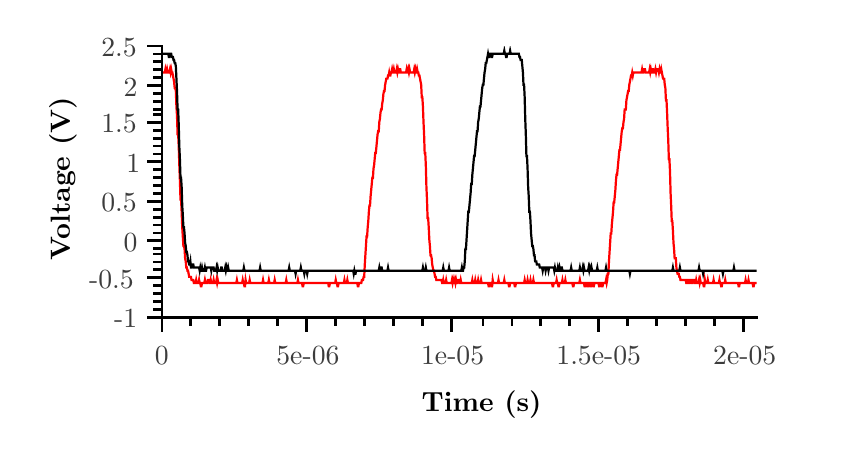
\begin{tikzpicture}{0pt}{0pt}{299pt}{150pt}
	\clip(0pt,150pt) -- (284.325pt,150pt) -- (284.325pt,7.36184pt) -- (0pt,7.36184pt) -- (0pt,150pt);
\begin{scope}
	\clip(48.497pt,143.344pt) -- (263.405pt,143.344pt) -- (263.405pt,45.3987pt) -- (48.497pt,45.3987pt) -- (48.497pt,143.344pt);
	\color[rgb]{1,0,0}
	\draw[line width=0.8pt, line join=miter, line cap=rect](48.7071pt,133.829pt) -- (48.9171pt,133.829pt) -- (49.1272pt,133.829pt) -- (49.3373pt,133.829pt) -- (49.5474pt,133.829pt) -- (49.7574pt,134.948pt) -- (49.9675pt,133.829pt) -- (50.1776pt,133.829pt) -- (50.3877pt,134.948pt) -- (50.5977pt,133.829pt) -- (50.8078pt,133.829pt) -- (51.0179pt,133.829pt) -- (51.228pt,133.829pt) -- (51.438pt,134.948pt) -- (51.6481pt,133.829pt) -- (51.8582pt,134.948pt) -- (52.0683pt,133.829pt) -- (52.2783pt,133.829pt) -- (52.4884pt,132.71pt) -- (52.6985pt,131.59pt) -- (52.9086pt,130.471pt) -- (53.1187pt,128.232pt) -- (53.3287pt,128.232pt) -- (53.5388pt,127.113pt) -- (53.7489pt,121.516pt) -- (53.959pt,118.158pt) -- (54.169pt,111.442pt) -- (54.3791pt,111.442pt) -- (54.5892pt,106.964pt) -- (54.7993pt,100.248pt) -- (55.0093pt,94.651pt) -- (55.2194pt,87.9347pt) -- (55.4295pt,87.9347pt) -- (55.6396pt,83.4573pt) -- (55.8496pt,77.8604pt) -- (56.0597pt,74.5023pt) -- (56.2698pt,71.1442pt) -- (56.4799pt,71.1442pt) -- (56.69pt,70.0248pt) -- (56.9pt,66.6667pt) -- (57.1101pt,65.5473pt) -- (57.3202pt,63.3086pt) -- (57.5303pt,63.3086pt) -- (57.7403pt,62.1892pt) -- (57.9504pt,62.1892pt) -- (58.1605pt,61.0699pt) -- (58.3706pt,59.9505pt) -- (58.5806pt,59.9505pt) -- (58.7907pt,59.9505pt) -- (59.0008pt,59.9505pt) -- (59.2109pt,58.8311pt) -- (59.4209pt,58.8311pt) -- (59.631pt,58.8311pt) -- (59.8411pt,58.8311pt) -- (60.0512pt,57.7118pt) -- (60.2613pt,57.7118pt) -- (60.4713pt,57.7118pt) -- (60.6814pt,57.7118pt) -- (60.8915pt,58.8311pt) -- (61.1016pt,57.7118pt) -- (61.3116pt,57.7118pt) -- (61.5217pt,57.7118pt) -- (61.7318pt,57.7118pt) -- (61.9419pt,58.8311pt) -- (62.1519pt,57.7118pt) -- (62.362pt,57.7118pt) -- (62.5721pt,56.5924pt) -- (62.7822pt,56.5924pt) -- (62.9922pt,57.7118pt) -- (63.2023pt,57.7118pt) -- (63.4124pt,57.7118pt) -- (63.6225pt,57.7118pt) -- (63.8326pt,57.7118pt) -- (64.0426pt,58.8311pt) -- (64.2527pt,57.7118pt) -- (64.4628pt,57.7118pt) -- (64.6729pt,57.7118pt) -- (64.8829pt,57.7118pt) -- (65.093pt,58.8311pt) -- (65.3031pt,58.8311pt) -- (65.5132pt,58.8311pt) -- (65.7232pt,57.7118pt) -- (65.9333pt,57.7118pt) -- (66.1434pt,58.8311pt) -- (66.3535pt,57.7118pt) -- (66.5635pt,57.7118pt) -- (66.7736pt,57.7118pt) -- (66.9837pt,57.7118pt) -- (67.1938pt,58.8311pt) -- (67.4038pt,57.7118pt) -- (67.6139pt,57.7118pt) -- (67.824pt,57.7118pt) -- (68.0341pt,57.7118pt) -- (68.2442pt,58.8311pt) -- (68.4542pt,57.7118pt) -- (68.6643pt,58.8311pt) -- (68.8744pt,57.7118pt) -- (69.0845pt,57.7118pt) -- (69.2945pt,57.7118pt) -- (69.5046pt,57.7118pt) -- (69.7147pt,57.7118pt) -- (69.9248pt,57.7118pt) -- (70.1348pt,57.7118pt) -- (70.3449pt,57.7118pt) -- (70.555pt,57.7118pt) -- (70.7651pt,57.7118pt) -- (70.9751pt,57.7118pt) -- (71.1852pt,57.7118pt) -- (71.3953pt,57.7118pt) -- (71.6054pt,57.7118pt) -- (71.8155pt,57.7118pt) -- (72.0255pt,57.7118pt) -- (72.2356pt,57.7118pt) -- (72.4457pt,57.7118pt) -- (72.6558pt,57.7118pt) -- (72.8658pt,57.7118pt) -- (73.0759pt,57.7118pt) -- (73.286pt,57.7118pt) -- (73.4961pt,57.7118pt) -- (73.7061pt,57.7118pt) -- (73.9162pt,57.7118pt) -- (74.1263pt,57.7118pt) -- (74.3364pt,57.7118pt) -- (74.5464pt,57.7118pt) -- (74.7565pt,57.7118pt) -- (74.9666pt,57.7118pt) -- (75.1767pt,57.7118pt) -- (75.3868pt,57.7118pt) -- (75.5968pt,58.8311pt) -- (75.8069pt,57.7118pt) -- (76.017pt,57.7118pt) -- (76.2271pt,57.7118pt) -- (76.4371pt,57.7118pt) -- (76.6472pt,57.7118pt) -- (76.8573pt,57.7118pt) -- (77.0674pt,57.7118pt) -- (77.2774pt,57.7118pt) -- (77.4875pt,57.7118pt) -- (77.6976pt,58.8311pt) -- (77.9077pt,57.7118pt) -- (78.1177pt,57.7118pt) -- (78.3278pt,56.5924pt) -- (78.5379pt,56.5924pt) -- (78.748pt,58.8311pt) -- (78.9581pt,57.7118pt) -- (79.1681pt,57.7118pt) -- (79.3782pt,57.7118pt) -- (79.5883pt,57.7118pt) -- (79.7984pt,57.7118pt) -- (80.0084pt,57.7118pt) -- (80.2185pt,58.8311pt) -- (80.4286pt,57.7118pt) -- (80.6387pt,57.7118pt) -- (80.8487pt,57.7118pt) -- (81.0588pt,57.7118pt) -- (81.2689pt,57.7118pt) -- (81.479pt,57.7118pt) -- (81.689pt,57.7118pt) -- (81.8991pt,57.7118pt) -- (82.1092pt,57.7118pt) -- (82.3193pt,57.7118pt) -- (82.5294pt,57.7118pt) -- (82.7394pt,57.7118pt) -- (82.9495pt,57.7118pt) -- (83.1596pt,57.7118pt) -- (83.3697pt,57.7118pt) -- (83.5797pt,57.7118pt) -- (83.7898pt,57.7118pt) -- (83.9999pt,57.7118pt) -- (84.21pt,57.7118pt) -- (84.42pt,57.7118pt) -- (84.6301pt,57.7118pt) -- (84.8402pt,57.7118pt) -- (85.0503pt,58.8311pt) -- (85.2603pt,57.7118pt) -- (85.4704pt,57.7118pt) -- (85.6805pt,57.7118pt) -- (85.8906pt,57.7118pt) -- (86.1006pt,57.7118pt) -- (86.3107pt,57.7118pt) -- (86.5208pt,57.7118pt) -- (86.7309pt,57.7118pt) -- (86.941pt,57.7118pt) -- (87.151pt,58.8311pt) -- (87.3611pt,57.7118pt) -- (87.5712pt,57.7118pt) -- (87.7813pt,57.7118pt) -- (87.9913pt,57.7118pt) -- (88.2014pt,57.7118pt) -- (88.4115pt,57.7118pt) -- (88.6216pt,57.7118pt) -- (88.8316pt,57.7118pt) -- (89.0417pt,57.7118pt) -- (89.2518pt,58.8311pt) -- (89.4619pt,57.7118pt) -- (89.6719pt,57.7118pt) -- (89.882pt,57.7118pt) -- (90.0921pt,57.7118pt) -- (90.3022pt,57.7118pt) -- (90.5123pt,57.7118pt) -- (90.7223pt,57.7118pt) -- (90.9324pt,57.7118pt) -- (91.1425pt,57.7118pt) -- (91.3526pt,57.7118pt) -- (91.5626pt,57.7118pt) -- (91.7727pt,57.7118pt) -- (91.9828pt,57.7118pt) -- (92.1929pt,57.7118pt) -- (92.4029pt,57.7118pt) -- (92.613pt,57.7118pt) -- (92.8231pt,57.7118pt) -- (93.0332pt,57.7118pt) -- (93.2432pt,57.7118pt) -- (93.4533pt,58.8311pt) -- (93.6634pt,57.7118pt) -- (93.8735pt,57.7118pt) -- (94.0836pt,57.7118pt) -- (94.2936pt,57.7118pt) -- (94.5037pt,57.7118pt) -- (94.7138pt,57.7118pt) -- (94.9239pt,57.7118pt) -- (95.1339pt,57.7118pt) -- (95.344pt,57.7118pt) -- (95.5541pt,57.7118pt) -- (95.7642pt,57.7118pt) -- (95.9742pt,57.7118pt) -- (96.1843pt,57.7118pt) -- (96.3944pt,57.7118pt) -- (96.6045pt,57.7118pt) -- (96.8145pt,57.7118pt) -- (97.0246pt,57.7118pt) -- (97.2347pt,57.7118pt) -- (97.4448pt,57.7118pt) -- (97.6549pt,58.8311pt) -- (97.8649pt,57.7118pt) -- (98.075pt,57.7118pt) -- (98.2851pt,57.7118pt) -- (98.4952pt,57.7118pt) -- (98.7052pt,57.7118pt) -- (98.9153pt,57.7118pt) -- (99.1254pt,57.7118pt) -- (99.3355pt,56.5924pt) -- (99.5455pt,56.5924pt) -- (99.7556pt,57.7118pt) -- (99.9657pt,57.7118pt) -- (100.176pt,57.7118pt) -- (100.386pt,57.7118pt) -- (100.596pt,57.7118pt) -- (100.806pt,57.7118pt) -- (101.016pt,57.7118pt) -- (101.226pt,57.7118pt) -- (101.436pt,57.7118pt) -- (101.646pt,57.7118pt) -- (101.856pt,57.7118pt) -- (102.066pt,57.7118pt) -- (102.277pt,57.7118pt) -- (102.487pt,57.7118pt) -- (102.697pt,57.7118pt) -- (102.907pt,57.7118pt) -- (103.117pt,57.7118pt) -- (103.327pt,57.7118pt) -- (103.537pt,57.7118pt) -- (103.747pt,57.7118pt) -- (103.957pt,57.7118pt) -- (104.167pt,57.7118pt) -- (104.377pt,57.7118pt) -- (104.587pt,57.7118pt) -- (104.797pt,57.7118pt) -- (105.008pt,57.7118pt) -- (105.218pt,57.7118pt) -- (105.428pt,57.7118pt) -- (105.638pt,57.7118pt) -- (105.848pt,57.7118pt) -- (106.058pt,57.7118pt) -- (106.268pt,57.7118pt) -- (106.478pt,57.7118pt) -- (106.688pt,57.7118pt) -- (106.898pt,57.7118pt) -- (107.108pt,57.7118pt) -- (107.318pt,57.7118pt) -- (107.528pt,57.7118pt) -- (107.739pt,57.7118pt) -- (107.949pt,57.7118pt) -- (108.159pt,57.7118pt) -- (108.369pt,57.7118pt) -- (108.579pt,57.7118pt) -- (108.789pt,56.5924pt) -- (108.999pt,56.5924pt) -- (109.209pt,57.7118pt) -- (109.419pt,57.7118pt) -- (109.629pt,57.7118pt) -- (109.839pt,57.7118pt) -- (110.049pt,57.7118pt) -- (110.259pt,57.7118pt) -- (110.47pt,57.7118pt) -- (110.68pt,57.7118pt) -- (110.89pt,57.7118pt) -- (111.1pt,57.7118pt) -- (111.31pt,58.8311pt) -- (111.52pt,57.7118pt) -- (111.73pt,57.7118pt) -- (111.94pt,56.5924pt) -- (112.15pt,56.5924pt) -- (112.36pt,57.7118pt) -- (112.57pt,57.7118pt) -- (112.78pt,57.7118pt) -- (112.99pt,57.7118pt) -- (113.201pt,57.7118pt) -- (113.411pt,57.7118pt) -- (113.621pt,57.7118pt) -- (113.831pt,57.7118pt) -- (114.041pt,57.7118pt) -- (114.251pt,57.7118pt) -- (114.461pt,58.8311pt) -- (114.671pt,57.7118pt) -- (114.881pt,57.7118pt) -- (115.091pt,57.7118pt) -- (115.301pt,57.7118pt) -- (115.511pt,58.8311pt) -- (115.721pt,57.7118pt) -- (115.931pt,57.7118pt) -- (116.142pt,57.7118pt) -- (116.352pt,57.7118pt) -- (116.562pt,57.7118pt) -- (116.772pt,57.7118pt) -- (116.982pt,57.7118pt) -- (117.192pt,57.7118pt) -- (117.402pt,57.7118pt) -- (117.612pt,57.7118pt) -- (117.822pt,57.7118pt) -- (118.032pt,57.7118pt) -- (118.242pt,57.7118pt) -- (118.452pt,57.7118pt) -- (118.662pt,57.7118pt) -- (118.873pt,57.7118pt) -- (119.083pt,57.7118pt) -- (119.293pt,56.5924pt) -- (119.503pt,56.5924pt) -- (119.713pt,57.7118pt) -- (119.923pt,57.7118pt) -- (120.133pt,57.7118pt) -- (120.343pt,57.7118pt) -- (120.553pt,57.7118pt) -- (120.763pt,58.8311pt) -- (120.973pt,58.8311pt) -- (121.183pt,58.8311pt) -- (121.393pt,59.9505pt) -- (121.604pt,59.9505pt) -- (121.814pt,64.428pt) -- (122.024pt,67.7861pt) -- (122.234pt,71.1442pt) -- (122.444pt,74.5023pt) -- (122.654pt,74.5023pt) -- (122.864pt,77.8604pt) -- (123.074pt,80.0992pt) -- (123.284pt,83.4573pt) -- (123.494pt,85.696pt) -- (123.704pt,85.696pt) -- (123.914pt,89.0541pt) -- (124.124pt,91.2929pt) -- (124.335pt,93.5316pt) -- (124.545pt,95.7703pt) -- (124.755pt,95.7703pt) -- (124.965pt,99.1284pt) -- (125.175pt,100.248pt) -- (125.385pt,102.487pt) -- (125.595pt,104.725pt) -- (125.805pt,104.725pt) -- (126.015pt,106.964pt) -- (126.225pt,109.203pt) -- (126.435pt,111.442pt) -- (126.645pt,112.561pt) -- (126.855pt,112.561pt) -- (127.066pt,115.919pt) -- (127.276pt,117.038pt) -- (127.486pt,119.277pt) -- (127.696pt,120.396pt) -- (127.906pt,120.396pt) -- (128.116pt,122.635pt) -- (128.326pt,123.755pt) -- (128.536pt,125.993pt) -- (128.746pt,127.113pt) -- (128.956pt,127.113pt) -- (129.166pt,129.351pt) -- (129.376pt,130.471pt) -- (129.586pt,131.59pt) -- (129.797pt,131.59pt) -- (130.007pt,131.59pt) -- (130.217pt,132.71pt) -- (130.427pt,132.71pt) -- (130.637pt,133.829pt) -- (130.847pt,132.71pt) -- (131.057pt,132.71pt) -- (131.267pt,133.829pt) -- (131.477pt,133.829pt) -- (131.687pt,134.948pt) -- (131.897pt,133.829pt) -- (132.107pt,133.829pt) -- (132.317pt,134.948pt) -- (132.528pt,133.829pt) -- (132.738pt,133.829pt) -- (132.948pt,133.829pt) -- (133.158pt,133.829pt) -- (133.368pt,134.948pt) -- (133.578pt,133.829pt) -- (133.788pt,134.948pt) -- (133.998pt,133.829pt) -- (134.208pt,133.829pt) -- (134.418pt,134.948pt) -- (134.628pt,134.948pt) -- (134.838pt,133.829pt) -- (135.048pt,133.829pt) -- (135.259pt,133.829pt) -- (135.469pt,133.829pt) -- (135.679pt,133.829pt) -- (135.889pt,133.829pt) -- (136.099pt,133.829pt) -- (136.309pt,133.829pt) -- (136.519pt,133.829pt) -- (136.729pt,133.829pt) -- (136.939pt,134.948pt) -- (137.149pt,133.829pt) -- (137.359pt,133.829pt) -- (137.569pt,134.948pt) -- (137.779pt,133.829pt) -- (137.99pt,134.948pt) -- (138.2pt,133.829pt) -- (138.41pt,133.829pt) -- (138.62pt,133.829pt) -- (138.83pt,133.829pt) -- (139.04pt,133.829pt) -- (139.25pt,133.829pt) -- (139.46pt,133.829pt) -- (139.67pt,134.948pt) -- (139.88pt,133.829pt) -- (140.09pt,134.948pt) -- (140.3pt,133.829pt) -- (140.51pt,133.829pt) -- (140.721pt,134.948pt) -- (140.931pt,133.829pt) -- (141.141pt,133.829pt) -- (141.351pt,132.71pt) -- (141.561pt,132.71pt) -- (141.771pt,131.59pt) -- (141.981pt,130.471pt) -- (142.191pt,129.351pt) -- (142.401pt,124.874pt) -- (142.611pt,124.874pt) -- (142.821pt,121.516pt) -- (143.031pt,115.919pt) -- (143.241pt,111.442pt) -- (143.452pt,104.725pt) -- (143.662pt,104.725pt) -- (143.872pt,100.248pt) -- (144.082pt,92.4122pt) -- (144.292pt,87.9347pt) -- (144.502pt,81.2185pt) -- (144.712pt,81.2185pt) -- (144.922pt,77.8604pt) -- (145.132pt,73.3829pt) -- (145.342pt,71.1442pt) -- (145.552pt,67.7861pt) -- (145.762pt,67.7861pt) -- (145.972pt,66.6667pt) -- (146.182pt,64.428pt) -- (146.393pt,63.3086pt) -- (146.603pt,62.1892pt) -- (146.813pt,62.1892pt) -- (147.023pt,61.0699pt) -- (147.233pt,59.9505pt) -- (147.443pt,59.9505pt) -- (147.653pt,58.8311pt) -- (147.863pt,58.8311pt) -- (148.073pt,58.8311pt) -- (148.283pt,58.8311pt) -- (148.493pt,58.8311pt) -- (148.703pt,58.8311pt) -- (148.913pt,58.8311pt) -- (149.124pt,58.8311pt) -- (149.334pt,58.8311pt) -- (149.544pt,58.8311pt) -- (149.754pt,57.7118pt) -- (149.964pt,57.7118pt) -- (150.174pt,58.8311pt) -- (150.384pt,57.7118pt) -- (150.594pt,57.7118pt) -- (150.804pt,57.7118pt) -- (151.014pt,57.7118pt) -- (151.224pt,58.8311pt) -- (151.434pt,57.7118pt) -- (151.644pt,57.7118pt) -- (151.855pt,57.7118pt) -- (152.065pt,57.7118pt) -- (152.275pt,57.7118pt) -- (152.485pt,57.7118pt) -- (152.695pt,57.7118pt) -- (152.905pt,57.7118pt) -- (153.115pt,57.7118pt) -- (153.325pt,58.8311pt) -- (153.535pt,57.7118pt) -- (153.745pt,58.8311pt) -- (153.955pt,57.7118pt) -- (154.165pt,57.7118pt) -- (154.375pt,58.8311pt) -- (154.586pt,57.7118pt) -- (154.796pt,58.8311pt) -- (155.006pt,57.7118pt) -- (155.216pt,57.7118pt) -- (155.426pt,58.8311pt) -- (155.636pt,58.8311pt) -- (155.846pt,58.8311pt) -- (156.056pt,57.7118pt) -- (156.266pt,57.7118pt) -- (156.476pt,58.8311pt) -- (156.686pt,57.7118pt) -- (156.896pt,57.7118pt) -- (157.106pt,57.7118pt) -- (157.317pt,57.7118pt) -- (157.527pt,57.7118pt) -- (157.737pt,57.7118pt) -- (157.947pt,57.7118pt) -- (158.157pt,57.7118pt) -- (158.367pt,57.7118pt) -- (158.577pt,57.7118pt) -- (158.787pt,57.7118pt) -- (158.997pt,57.7118pt) -- (159.207pt,57.7118pt) -- (159.417pt,57.7118pt) -- (159.627pt,57.7118pt) -- (159.837pt,57.7118pt) -- (160.048pt,57.7118pt) -- (160.258pt,57.7118pt) -- (160.468pt,57.7118pt) -- (160.678pt,58.8311pt) -- (160.888pt,57.7118pt) -- (161.098pt,57.7118pt) -- (161.308pt,57.7118pt) -- (161.518pt,57.7118pt) -- (161.728pt,58.8311pt) -- (161.938pt,57.7118pt) -- (162.148pt,57.7118pt) -- (162.358pt,57.7118pt) -- (162.568pt,57.7118pt) -- (162.779pt,58.8311pt) -- (162.989pt,57.7118pt) -- (163.199pt,57.7118pt) -- (163.409pt,57.7118pt) -- (163.619pt,57.7118pt) -- (163.829pt,58.8311pt) -- (164.039pt,57.7118pt) -- (164.249pt,57.7118pt) -- (164.459pt,57.7118pt) -- (164.669pt,57.7118pt) -- (164.879pt,57.7118pt) -- (165.089pt,57.7118pt) -- (165.299pt,57.7118pt) -- (165.51pt,57.7118pt) -- (165.72pt,57.7118pt) -- (165.93pt,57.7118pt) -- (166.14pt,57.7118pt) -- (166.35pt,57.7118pt) -- (166.56pt,56.5924pt) -- (166.77pt,56.5924pt) -- (166.98pt,57.7118pt) -- (167.19pt,57.7118pt) -- (167.4pt,57.7118pt) -- (167.61pt,56.5924pt) -- (167.82pt,56.5924pt) -- (168.03pt,58.8311pt) -- (168.241pt,57.7118pt) -- (168.451pt,57.7118pt) -- (168.661pt,57.7118pt) -- (168.871pt,57.7118pt) -- (169.081pt,57.7118pt) -- (169.291pt,57.7118pt) -- (169.501pt,57.7118pt) -- (169.711pt,57.7118pt) -- (169.921pt,57.7118pt) -- (170.131pt,58.8311pt) -- (170.341pt,57.7118pt) -- (170.551pt,57.7118pt) -- (170.761pt,57.7118pt) -- (170.972pt,57.7118pt) -- (171.182pt,57.7118pt) -- (171.392pt,57.7118pt) -- (171.602pt,57.7118pt) -- (171.812pt,57.7118pt) -- (172.022pt,57.7118pt) -- (172.232pt,58.8311pt) -- (172.442pt,57.7118pt) -- (172.652pt,57.7118pt) -- (172.862pt,57.7118pt) -- (173.072pt,57.7118pt) -- (173.282pt,57.7118pt) -- (173.492pt,57.7118pt) -- (173.703pt,57.7118pt) -- (173.913pt,56.5924pt) -- (174.123pt,56.5924pt) -- (174.333pt,57.7118pt) -- (174.543pt,57.7118pt) -- (174.753pt,57.7118pt) -- (174.963pt,57.7118pt) -- (175.173pt,57.7118pt) -- (175.383pt,57.7118pt) -- (175.593pt,57.7118pt) -- (175.803pt,57.7118pt) -- (176.013pt,56.5924pt) -- (176.223pt,56.5924pt) -- (176.434pt,57.7118pt) -- (176.644pt,57.7118pt) -- (176.854pt,57.7118pt) -- (177.064pt,57.7118pt) -- (177.274pt,57.7118pt) -- (177.484pt,57.7118pt) -- (177.694pt,57.7118pt) -- (177.904pt,57.7118pt) -- (178.114pt,57.7118pt) -- (178.324pt,57.7118pt) -- (178.534pt,57.7118pt) -- (178.744pt,57.7118pt) -- (178.954pt,57.7118pt) -- (179.164pt,57.7118pt) -- (179.375pt,57.7118pt) -- (179.585pt,58.8311pt) -- (179.795pt,57.7118pt) -- (180.005pt,57.7118pt) -- (180.215pt,57.7118pt) -- (180.425pt,57.7118pt) -- (180.635pt,58.8311pt) -- (180.845pt,57.7118pt) -- (181.055pt,57.7118pt) -- (181.265pt,57.7118pt) -- (181.475pt,57.7118pt) -- (181.685pt,58.8311pt) -- (181.895pt,57.7118pt) -- (182.106pt,57.7118pt) -- (182.316pt,57.7118pt) -- (182.526pt,57.7118pt) -- (182.736pt,58.8311pt) -- (182.946pt,57.7118pt) -- (183.156pt,57.7118pt) -- (183.366pt,57.7118pt) -- (183.576pt,57.7118pt) -- (183.786pt,57.7118pt) -- (183.996pt,57.7118pt) -- (184.206pt,57.7118pt) -- (184.416pt,57.7118pt) -- (184.626pt,57.7118pt) -- (184.837pt,57.7118pt) -- (185.047pt,57.7118pt) -- (185.257pt,57.7118pt) -- (185.467pt,57.7118pt) -- (185.677pt,57.7118pt) -- (185.887pt,57.7118pt) -- (186.097pt,57.7118pt) -- (186.307pt,57.7118pt) -- (186.517pt,57.7118pt) -- (186.727pt,57.7118pt) -- (186.937pt,57.7118pt) -- (187.147pt,57.7118pt) -- (187.357pt,57.7118pt) -- (187.568pt,57.7118pt) -- (187.778pt,57.7118pt) -- (187.988pt,57.7118pt) -- (188.198pt,57.7118pt) -- (188.408pt,57.7118pt) -- (188.618pt,57.7118pt) -- (188.828pt,57.7118pt) -- (189.038pt,57.7118pt) -- (189.248pt,57.7118pt) -- (189.458pt,57.7118pt) -- (189.668pt,56.5924pt) -- (189.878pt,56.5924pt) -- (190.088pt,57.7118pt) -- (190.299pt,57.7118pt) -- (190.509pt,57.7118pt) -- (190.719pt,57.7118pt) -- (190.929pt,57.7118pt) -- (191.139pt,58.8311pt) -- (191.349pt,57.7118pt) -- (191.559pt,57.7118pt) -- (191.769pt,56.5924pt) -- (191.979pt,56.5924pt) -- (192.189pt,57.7118pt) -- (192.399pt,57.7118pt) -- (192.609pt,57.7118pt) -- (192.819pt,57.7118pt) -- (193.03pt,57.7118pt) -- (193.24pt,58.8311pt) -- (193.45pt,57.7118pt) -- (193.66pt,57.7118pt) -- (193.87pt,57.7118pt) -- (194.08pt,57.7118pt) -- (194.29pt,58.8311pt) -- (194.5pt,57.7118pt) -- (194.71pt,57.7118pt) -- (194.92pt,57.7118pt) -- (195.13pt,57.7118pt) -- (195.34pt,57.7118pt) -- (195.55pt,57.7118pt) -- (195.761pt,57.7118pt) -- (195.971pt,57.7118pt) -- (196.181pt,57.7118pt) -- (196.391pt,57.7118pt) -- (196.601pt,57.7118pt) -- (196.811pt,57.7118pt) -- (197.021pt,56.5924pt) -- (197.231pt,56.5924pt) -- (197.441pt,57.7118pt) -- (197.651pt,57.7118pt) -- (197.861pt,57.7118pt) -- (198.071pt,57.7118pt) -- (198.281pt,57.7118pt) -- (198.492pt,57.7118pt) -- (198.702pt,57.7118pt) -- (198.912pt,57.7118pt) -- (199.122pt,57.7118pt) -- (199.332pt,57.7118pt) -- (199.542pt,58.8311pt) -- (199.752pt,57.7118pt) -- (199.962pt,57.7118pt) -- (200.172pt,57.7118pt) -- (200.382pt,57.7118pt) -- (200.592pt,57.7118pt) -- (200.802pt,57.7118pt) -- (201.012pt,57.7118pt) -- (201.223pt,56.5924pt) -- (201.433pt,56.5924pt) -- (201.643pt,57.7118pt) -- (201.853pt,57.7118pt) -- (202.063pt,57.7118pt) -- (202.273pt,56.5924pt) -- (202.483pt,56.5924pt) -- (202.693pt,57.7118pt) -- (202.903pt,57.7118pt) -- (203.113pt,57.7118pt) -- (203.323pt,56.5924pt) -- (203.533pt,56.5924pt) -- (203.743pt,57.7118pt) -- (203.954pt,57.7118pt) -- (204.164pt,57.7118pt) -- (204.374pt,56.5924pt) -- (204.584pt,56.5924pt) -- (204.794pt,57.7118pt) -- (205.004pt,57.7118pt) -- (205.214pt,57.7118pt) -- (205.424pt,57.7118pt) -- (205.634pt,57.7118pt) -- (205.844pt,57.7118pt) -- (206.054pt,57.7118pt) -- (206.264pt,57.7118pt) -- (206.474pt,56.5924pt) -- (206.685pt,56.5924pt) -- (206.895pt,57.7118pt) -- (207.105pt,57.7118pt) -- (207.315pt,57.7118pt) -- (207.525pt,56.5924pt) -- (207.735pt,56.5924pt) -- (207.945pt,57.7118pt) -- (208.155pt,57.7118pt) -- (208.365pt,57.7118pt) -- (208.575pt,57.7118pt) -- (208.785pt,57.7118pt) -- (208.995pt,58.8311pt) -- (209.205pt,57.7118pt) -- (209.415pt,58.8311pt) -- (209.626pt,61.0699pt) -- (209.836pt,61.0699pt) -- (210.046pt,65.5473pt) -- (210.256pt,68.9055pt) -- (210.466pt,72.2636pt) -- (210.676pt,75.6217pt) -- (210.886pt,75.6217pt) -- (211.096pt,78.9798pt) -- (211.306pt,81.2185pt) -- (211.516pt,83.4573pt) -- (211.726pt,86.8154pt) -- (211.936pt,86.8154pt) -- (212.146pt,89.0541pt) -- (212.357pt,91.2929pt) -- (212.567pt,94.651pt) -- (212.777pt,96.8897pt) -- (212.987pt,96.8897pt) -- (213.197pt,99.1284pt) -- (213.407pt,101.367pt) -- (213.617pt,103.606pt) -- (213.827pt,105.845pt) -- (214.037pt,105.845pt) -- (214.247pt,108.083pt) -- (214.457pt,110.322pt) -- (214.667pt,112.561pt) -- (214.877pt,113.68pt) -- (215.088pt,113.68pt) -- (215.298pt,115.919pt) -- (215.508pt,117.038pt) -- (215.718pt,120.396pt) -- (215.928pt,120.396pt) -- (216.138pt,120.396pt) -- (216.348pt,123.755pt) -- (216.558pt,124.874pt) -- (216.768pt,125.993pt) -- (216.978pt,127.113pt) -- (217.188pt,127.113pt) -- (217.398pt,129.351pt) -- (217.608pt,130.471pt) -- (217.819pt,131.59pt) -- (218.029pt,132.71pt) -- (218.239pt,132.71pt) -- (218.449pt,133.829pt) -- (218.659pt,132.71pt) -- (218.869pt,133.829pt) -- (219.079pt,133.829pt) -- (219.289pt,133.829pt) -- (219.499pt,133.829pt) -- (219.709pt,133.829pt) -- (219.919pt,133.829pt) -- (220.129pt,133.829pt) -- (220.339pt,133.829pt) -- (220.55pt,133.829pt) -- (220.76pt,133.829pt) -- (220.97pt,133.829pt) -- (221.18pt,133.829pt) -- (221.39pt,133.829pt) -- (221.6pt,133.829pt) -- (221.81pt,133.829pt) -- (222.02pt,134.948pt) -- (222.23pt,133.829pt) -- (222.44pt,133.829pt) -- (222.65pt,134.948pt) -- (222.86pt,134.948pt) -- (223.07pt,134.948pt) -- (223.281pt,133.829pt) -- (223.491pt,133.829pt) -- (223.701pt,133.829pt) -- (223.911pt,133.829pt) -- (224.121pt,133.829pt) -- (224.331pt,133.829pt) -- (224.541pt,133.829pt) -- (224.751pt,134.948pt) -- (224.961pt,133.829pt) -- (225.171pt,134.948pt) -- (225.381pt,133.829pt) -- (225.591pt,133.829pt) -- (225.801pt,134.948pt) -- (226.012pt,134.948pt) -- (226.222pt,133.829pt) -- (226.432pt,133.829pt) -- (226.642pt,133.829pt) -- (226.852pt,134.948pt) -- (227.062pt,133.829pt) -- (227.272pt,134.948pt) -- (227.482pt,134.948pt) -- (227.692pt,134.948pt) -- (227.902pt,134.948pt) -- (228.112pt,133.829pt) -- (228.322pt,134.948pt) -- (228.532pt,133.829pt) -- (228.743pt,133.829pt) -- (228.953pt,134.948pt) -- (229.163pt,133.829pt) -- (229.373pt,132.71pt) -- (229.583pt,131.59pt) -- (229.793pt,131.59pt) -- (230.003pt,131.59pt) -- (230.213pt,129.351pt) -- (230.423pt,128.232pt) -- (230.633pt,123.755pt) -- (230.843pt,123.755pt) -- (231.053pt,119.277pt) -- (231.263pt,113.68pt) -- (231.474pt,109.203pt) -- (231.684pt,102.487pt) -- (231.894pt,102.487pt) -- (232.104pt,98.0091pt) -- (232.314pt,90.1735pt) -- (232.524pt,85.696pt) -- (232.734pt,80.0992pt) -- (232.944pt,80.0992pt) -- (233.154pt,76.741pt) -- (233.364pt,72.2636pt) -- (233.574pt,70.0248pt) -- (233.784pt,66.6667pt) -- (233.994pt,66.6667pt) -- (234.205pt,66.6667pt) -- (234.415pt,63.3086pt) -- (234.625pt,62.1892pt) -- (234.835pt,61.0699pt) -- (235.045pt,61.0699pt) -- (235.255pt,61.0699pt) -- (235.465pt,59.9505pt) -- (235.675pt,59.9505pt) -- (235.885pt,58.8311pt) -- (236.095pt,58.8311pt) -- (236.305pt,58.8311pt) -- (236.515pt,58.8311pt) -- (236.725pt,58.8311pt) -- (236.936pt,58.8311pt) -- (237.146pt,58.8311pt) -- (237.356pt,58.8311pt) -- (237.566pt,58.8311pt) -- (237.776pt,58.8311pt) -- (237.986pt,57.7118pt) -- (238.196pt,57.7118pt) -- (238.406pt,58.8311pt) -- (238.616pt,58.8311pt) -- (238.826pt,58.8311pt) -- (239.036pt,57.7118pt) -- (239.246pt,57.7118pt) -- (239.456pt,58.8311pt) -- (239.666pt,58.8311pt) -- (239.877pt,58.8311pt) -- (240.087pt,57.7118pt) -- (240.297pt,57.7118pt) -- (240.507pt,58.8311pt) -- (240.717pt,58.8311pt) -- (240.927pt,58.8311pt) -- (241.137pt,57.7118pt) -- (241.347pt,57.7118pt) -- (241.557pt,58.8311pt) -- (241.767pt,57.7118pt) -- (241.977pt,57.7118pt) -- (242.187pt,57.7118pt) -- (242.397pt,57.7118pt) -- (242.608pt,58.8311pt) -- (242.818pt,57.7118pt) -- (243.028pt,58.8311pt) -- (243.238pt,57.7118pt) -- (243.448pt,57.7118pt) -- (243.658pt,57.7118pt) -- (243.868pt,57.7118pt) -- (244.078pt,57.7118pt) -- (244.288pt,56.5924pt) -- (244.498pt,56.5924pt) -- (244.708pt,58.8311pt) -- (244.918pt,57.7118pt) -- (245.128pt,57.7118pt) -- (245.339pt,57.7118pt) -- (245.549pt,57.7118pt) -- (245.759pt,58.8311pt) -- (245.969pt,57.7118pt) -- (246.179pt,57.7118pt) -- (246.389pt,57.7118pt) -- (246.599pt,57.7118pt) -- (246.809pt,57.7118pt) -- (247.019pt,57.7118pt) -- (247.229pt,57.7118pt) -- (247.439pt,57.7118pt) -- (247.649pt,57.7118pt) -- (247.859pt,58.8311pt) -- (248.07pt,57.7118pt) -- (248.28pt,57.7118pt) -- (248.49pt,57.7118pt) -- (248.7pt,57.7118pt) -- (248.91pt,57.7118pt) -- (249.12pt,57.7118pt) -- (249.33pt,57.7118pt) -- (249.54pt,57.7118pt) -- (249.75pt,57.7118pt) -- (249.96pt,58.8311pt) -- (250.17pt,57.7118pt) -- (250.38pt,57.7118pt) -- (250.59pt,56.5924pt) -- (250.801pt,56.5924pt) -- (251.011pt,57.7118pt) -- (251.221pt,57.7118pt) -- (251.431pt,57.7118pt) -- (251.641pt,57.7118pt) -- (251.851pt,57.7118pt) -- (252.061pt,58.8311pt) -- (252.271pt,57.7118pt) -- (252.481pt,57.7118pt) -- (252.691pt,57.7118pt) -- (252.901pt,57.7118pt) -- (253.111pt,57.7118pt) -- (253.321pt,57.7118pt) -- (253.532pt,57.7118pt) -- (253.742pt,57.7118pt) -- (253.952pt,57.7118pt) -- (254.162pt,57.7118pt) -- (254.372pt,57.7118pt) -- (254.582pt,57.7118pt) -- (254.792pt,57.7118pt) -- (255.002pt,57.7118pt) -- (255.212pt,57.7118pt) -- (255.422pt,57.7118pt) -- (255.632pt,57.7118pt) -- (255.842pt,57.7118pt) -- (256.052pt,57.7118pt) -- (256.263pt,57.7118pt) -- (256.473pt,57.7118pt) -- (256.683pt,57.7118pt) -- (256.893pt,56.5924pt) -- (257.103pt,56.5924pt) -- (257.313pt,57.7118pt) -- (257.523pt,57.7118pt) -- (257.733pt,57.7118pt) -- (257.943pt,57.7118pt) -- (258.153pt,57.7118pt) -- (258.363pt,57.7118pt) -- (258.573pt,57.7118pt) -- (258.783pt,57.7118pt) -- (258.994pt,57.7118pt) -- (259.204pt,57.7118pt) -- (259.414pt,58.8311pt) -- (259.624pt,57.7118pt) -- (259.834pt,57.7118pt) -- (260.044pt,57.7118pt) -- (260.254pt,57.7118pt) -- (260.464pt,58.8311pt) -- (260.674pt,57.7118pt) -- (260.884pt,57.7118pt) -- (261.094pt,57.7118pt) -- (261.304pt,57.7118pt) -- (261.514pt,57.7118pt) -- (261.725pt,57.7118pt) -- (261.935pt,57.7118pt) -- (262.145pt,56.5924pt) -- (262.355pt,56.5924pt) -- (262.565pt,57.7118pt) -- (262.775pt,57.7118pt) -- (262.985pt,57.7118pt) -- (263.195pt,57.7118pt) -- (263.405pt,57.7118pt);
	\color[rgb]{0,0,0}
	\draw[line width=0.8pt, line join=miter, line cap=rect](48.7071pt,140.545pt) -- (48.9171pt,140.545pt) -- (49.1272pt,140.545pt) -- (49.3373pt,140.545pt) -- (49.5474pt,140.545pt) -- (49.7574pt,140.545pt) -- (49.9675pt,140.545pt) -- (50.1776pt,140.545pt) -- (50.3877pt,140.545pt) -- (50.5977pt,140.545pt) -- (50.8078pt,140.545pt) -- (51.0179pt,139.426pt) -- (51.228pt,139.426pt) -- (51.438pt,140.545pt) -- (51.6481pt,140.545pt) -- (51.8582pt,140.545pt) -- (52.0683pt,139.426pt) -- (52.2783pt,139.426pt) -- (52.4884pt,139.426pt) -- (52.6985pt,138.306pt) -- (52.9086pt,138.306pt) -- (53.1187pt,137.187pt) -- (53.3287pt,137.187pt) -- (53.5388pt,136.068pt) -- (53.7489pt,131.59pt) -- (53.959pt,127.113pt) -- (54.169pt,120.396pt) -- (54.3791pt,120.396pt) -- (54.5892pt,114.8pt) -- (54.7993pt,106.964pt) -- (55.0093pt,102.487pt) -- (55.2194pt,95.7703pt) -- (55.4295pt,95.7703pt) -- (55.6396pt,92.4122pt) -- (55.8496pt,85.696pt) -- (56.0597pt,82.3379pt) -- (56.2698pt,77.8604pt) -- (56.4799pt,77.8604pt) -- (56.69pt,75.6217pt) -- (56.9pt,72.2636pt) -- (57.1101pt,71.1442pt) -- (57.3202pt,68.9055pt) -- (57.5303pt,68.9055pt) -- (57.7403pt,67.7861pt) -- (57.9504pt,65.5473pt) -- (58.1605pt,65.5473pt) -- (58.3706pt,64.428pt) -- (58.5806pt,64.428pt) -- (58.7907pt,65.5473pt) -- (59.0008pt,63.3086pt) -- (59.2109pt,63.3086pt) -- (59.4209pt,64.428pt) -- (59.631pt,64.428pt) -- (59.8411pt,64.428pt) -- (60.0512pt,63.3086pt) -- (60.2613pt,63.3086pt) -- (60.4713pt,63.3086pt) -- (60.6814pt,63.3086pt) -- (60.8915pt,63.3086pt) -- (61.1016pt,63.3086pt) -- (61.3116pt,63.3086pt) -- (61.5217pt,63.3086pt) -- (61.7318pt,63.3086pt) -- (61.9419pt,63.3086pt) -- (62.1519pt,62.1892pt) -- (62.362pt,63.3086pt) -- (62.5721pt,62.1892pt) -- (62.7822pt,62.1892pt) -- (62.9922pt,63.3086pt) -- (63.2023pt,62.1892pt) -- (63.4124pt,62.1892pt) -- (63.6225pt,62.1892pt) -- (63.8326pt,62.1892pt) -- (64.0426pt,63.3086pt) -- (64.2527pt,62.1892pt) -- (64.4628pt,62.1892pt) -- (64.6729pt,63.3086pt) -- (64.8829pt,63.3086pt) -- (65.093pt,63.3086pt) -- (65.3031pt,63.3086pt) -- (65.5132pt,63.3086pt) -- (65.7232pt,63.3086pt) -- (65.9333pt,63.3086pt) -- (66.1434pt,63.3086pt) -- (66.3535pt,62.1892pt) -- (66.5635pt,63.3086pt) -- (66.7736pt,63.3086pt) -- (66.9837pt,63.3086pt) -- (67.1938pt,63.3086pt) -- (67.4038pt,62.1892pt) -- (67.6139pt,62.1892pt) -- (67.824pt,62.1892pt) -- (68.0341pt,62.1892pt) -- (68.2442pt,63.3086pt) -- (68.4542pt,62.1892pt) -- (68.6643pt,63.3086pt) -- (68.8744pt,62.1892pt) -- (69.0845pt,62.1892pt) -- (69.2945pt,62.1892pt) -- (69.5046pt,62.1892pt) -- (69.7147pt,62.1892pt) -- (69.9248pt,63.3086pt) -- (70.1348pt,63.3086pt) -- (70.3449pt,62.1892pt) -- (70.555pt,62.1892pt) -- (70.7651pt,62.1892pt) -- (70.9751pt,62.1892pt) -- (71.1852pt,62.1892pt) -- (71.3953pt,63.3086pt) -- (71.6054pt,62.1892pt) -- (71.8155pt,63.3086pt) -- (72.0255pt,62.1892pt) -- (72.2356pt,62.1892pt) -- (72.4457pt,63.3086pt) -- (72.6558pt,62.1892pt) -- (72.8658pt,62.1892pt) -- (73.0759pt,62.1892pt) -- (73.286pt,62.1892pt) -- (73.4961pt,62.1892pt) -- (73.7061pt,62.1892pt) -- (73.9162pt,62.1892pt) -- (74.1263pt,62.1892pt) -- (74.3364pt,62.1892pt) -- (74.5464pt,62.1892pt) -- (74.7565pt,62.1892pt) -- (74.9666pt,62.1892pt) -- (75.1767pt,62.1892pt) -- (75.3868pt,62.1892pt) -- (75.5968pt,62.1892pt) -- (75.8069pt,62.1892pt) -- (76.017pt,62.1892pt) -- (76.2271pt,62.1892pt) -- (76.4371pt,62.1892pt) -- (76.6472pt,62.1892pt) -- (76.8573pt,62.1892pt) -- (77.0674pt,62.1892pt) -- (77.2774pt,62.1892pt) -- (77.4875pt,62.1892pt) -- (77.6976pt,62.1892pt) -- (77.9077pt,62.1892pt) -- (78.1177pt,63.3086pt) -- (78.3278pt,62.1892pt) -- (78.5379pt,62.1892pt) -- (78.748pt,62.1892pt) -- (78.9581pt,62.1892pt) -- (79.1681pt,62.1892pt) -- (79.3782pt,62.1892pt) -- (79.5883pt,62.1892pt) -- (79.7984pt,62.1892pt) -- (80.0084pt,62.1892pt) -- (80.2185pt,62.1892pt) -- (80.4286pt,62.1892pt) -- (80.6387pt,62.1892pt) -- (80.8487pt,62.1892pt) -- (81.0588pt,62.1892pt) -- (81.2689pt,62.1892pt) -- (81.479pt,62.1892pt) -- (81.689pt,62.1892pt) -- (81.8991pt,62.1892pt) -- (82.1092pt,62.1892pt) -- (82.3193pt,62.1892pt) -- (82.5294pt,62.1892pt) -- (82.7394pt,62.1892pt) -- (82.9495pt,62.1892pt) -- (83.1596pt,62.1892pt) -- (83.3697pt,62.1892pt) -- (83.5797pt,62.1892pt) -- (83.7898pt,62.1892pt) -- (83.9999pt,63.3086pt) -- (84.21pt,62.1892pt) -- (84.42pt,62.1892pt) -- (84.6301pt,62.1892pt) -- (84.8402pt,62.1892pt) -- (85.0503pt,62.1892pt) -- (85.2603pt,62.1892pt) -- (85.4704pt,62.1892pt) -- (85.6805pt,62.1892pt) -- (85.8906pt,62.1892pt) -- (86.1006pt,62.1892pt) -- (86.3107pt,62.1892pt) -- (86.5208pt,62.1892pt) -- (86.7309pt,62.1892pt) -- (86.941pt,62.1892pt) -- (87.151pt,62.1892pt) -- (87.3611pt,62.1892pt) -- (87.5712pt,62.1892pt) -- (87.7813pt,62.1892pt) -- (87.9913pt,62.1892pt) -- (88.2014pt,62.1892pt) -- (88.4115pt,62.1892pt) -- (88.6216pt,62.1892pt) -- (88.8316pt,62.1892pt) -- (89.0417pt,62.1892pt) -- (89.2518pt,62.1892pt) -- (89.4619pt,62.1892pt) -- (89.6719pt,62.1892pt) -- (89.882pt,62.1892pt) -- (90.0921pt,62.1892pt) -- (90.3022pt,62.1892pt) -- (90.5123pt,62.1892pt) -- (90.7223pt,62.1892pt) -- (90.9324pt,62.1892pt) -- (91.1425pt,62.1892pt) -- (91.3526pt,62.1892pt) -- (91.5626pt,62.1892pt) -- (91.7727pt,62.1892pt) -- (91.9828pt,62.1892pt) -- (92.1929pt,62.1892pt) -- (92.4029pt,62.1892pt) -- (92.613pt,62.1892pt) -- (92.8231pt,62.1892pt) -- (93.0332pt,62.1892pt) -- (93.2432pt,62.1892pt) -- (93.4533pt,62.1892pt) -- (93.6634pt,62.1892pt) -- (93.8735pt,62.1892pt) -- (94.0836pt,62.1892pt) -- (94.2936pt,62.1892pt) -- (94.5037pt,63.3086pt) -- (94.7138pt,62.1892pt) -- (94.9239pt,62.1892pt) -- (95.1339pt,62.1892pt) -- (95.344pt,62.1892pt) -- (95.5541pt,62.1892pt) -- (95.7642pt,62.1892pt) -- (95.9742pt,62.1892pt) -- (96.1843pt,62.1892pt) -- (96.3944pt,62.1892pt) -- (96.6045pt,62.1892pt) -- (96.8145pt,61.0699pt) -- (97.0246pt,62.1892pt) -- (97.2347pt,62.1892pt) -- (97.4448pt,62.1892pt) -- (97.6549pt,62.1892pt) -- (97.8649pt,62.1892pt) -- (98.075pt,62.1892pt) -- (98.2851pt,62.1892pt) -- (98.4952pt,62.1892pt) -- (98.7052pt,63.3086pt) -- (98.9153pt,62.1892pt) -- (99.1254pt,62.1892pt) -- (99.3355pt,62.1892pt) -- (99.5455pt,62.1892pt) -- (99.7556pt,62.1892pt) -- (99.9657pt,61.0699pt) -- (100.176pt,62.1892pt) -- (100.386pt,62.1892pt) -- (100.596pt,62.1892pt) -- (100.806pt,62.1892pt) -- (101.016pt,61.0699pt) -- (101.226pt,62.1892pt) -- (101.436pt,62.1892pt) -- (101.646pt,62.1892pt) -- (101.856pt,62.1892pt) -- (102.066pt,62.1892pt) -- (102.277pt,62.1892pt) -- (102.487pt,62.1892pt) -- (102.697pt,62.1892pt) -- (102.907pt,62.1892pt) -- (103.117pt,62.1892pt) -- (103.327pt,62.1892pt) -- (103.537pt,62.1892pt) -- (103.747pt,62.1892pt) -- (103.957pt,62.1892pt) -- (104.167pt,62.1892pt) -- (104.377pt,62.1892pt) -- (104.587pt,62.1892pt) -- (104.797pt,62.1892pt) -- (105.008pt,62.1892pt) -- (105.218pt,62.1892pt) -- (105.428pt,62.1892pt) -- (105.638pt,62.1892pt) -- (105.848pt,62.1892pt) -- (106.058pt,62.1892pt) -- (106.268pt,62.1892pt) -- (106.478pt,62.1892pt) -- (106.688pt,62.1892pt) -- (106.898pt,62.1892pt) -- (107.108pt,62.1892pt) -- (107.318pt,62.1892pt) -- (107.528pt,62.1892pt) -- (107.739pt,62.1892pt) -- (107.949pt,62.1892pt) -- (108.159pt,62.1892pt) -- (108.369pt,62.1892pt) -- (108.579pt,62.1892pt) -- (108.789pt,62.1892pt) -- (108.999pt,62.1892pt) -- (109.209pt,62.1892pt) -- (109.419pt,62.1892pt) -- (109.629pt,62.1892pt) -- (109.839pt,62.1892pt) -- (110.049pt,62.1892pt) -- (110.259pt,62.1892pt) -- (110.47pt,62.1892pt) -- (110.68pt,62.1892pt) -- (110.89pt,62.1892pt) -- (111.1pt,62.1892pt) -- (111.31pt,62.1892pt) -- (111.52pt,62.1892pt) -- (111.73pt,62.1892pt) -- (111.94pt,62.1892pt) -- (112.15pt,62.1892pt) -- (112.36pt,62.1892pt) -- (112.57pt,62.1892pt) -- (112.78pt,62.1892pt) -- (112.99pt,62.1892pt) -- (113.201pt,62.1892pt) -- (113.411pt,62.1892pt) -- (113.621pt,62.1892pt) -- (113.831pt,62.1892pt) -- (114.041pt,62.1892pt) -- (114.251pt,62.1892pt) -- (114.461pt,62.1892pt) -- (114.671pt,62.1892pt) -- (114.881pt,62.1892pt) -- (115.091pt,62.1892pt) -- (115.301pt,62.1892pt) -- (115.511pt,62.1892pt) -- (115.721pt,62.1892pt) -- (115.931pt,62.1892pt) -- (116.142pt,62.1892pt) -- (116.352pt,62.1892pt) -- (116.562pt,62.1892pt) -- (116.772pt,62.1892pt) -- (116.982pt,62.1892pt) -- (117.192pt,62.1892pt) -- (117.402pt,62.1892pt) -- (117.612pt,62.1892pt) -- (117.822pt,61.0699pt) -- (118.032pt,62.1892pt) -- (118.242pt,61.0699pt) -- (118.452pt,61.0699pt) -- (118.662pt,62.1892pt) -- (118.873pt,62.1892pt) -- (119.083pt,62.1892pt) -- (119.293pt,62.1892pt) -- (119.503pt,62.1892pt) -- (119.713pt,62.1892pt) -- (119.923pt,62.1892pt) -- (120.133pt,62.1892pt) -- (120.343pt,62.1892pt) -- (120.553pt,62.1892pt) -- (120.763pt,62.1892pt) -- (120.973pt,62.1892pt) -- (121.183pt,62.1892pt) -- (121.393pt,62.1892pt) -- (121.604pt,62.1892pt) -- (121.814pt,62.1892pt) -- (122.024pt,62.1892pt) -- (122.234pt,62.1892pt) -- (122.444pt,62.1892pt) -- (122.654pt,62.1892pt) -- (122.864pt,62.1892pt) -- (123.074pt,62.1892pt) -- (123.284pt,62.1892pt) -- (123.494pt,62.1892pt) -- (123.704pt,62.1892pt) -- (123.914pt,62.1892pt) -- (124.124pt,62.1892pt) -- (124.335pt,62.1892pt) -- (124.545pt,62.1892pt) -- (124.755pt,62.1892pt) -- (124.965pt,62.1892pt) -- (125.175pt,62.1892pt) -- (125.385pt,62.1892pt) -- (125.595pt,62.1892pt) -- (125.805pt,62.1892pt) -- (126.015pt,62.1892pt) -- (126.225pt,62.1892pt) -- (126.435pt,62.1892pt) -- (126.645pt,62.1892pt) -- (126.855pt,62.1892pt) -- (127.066pt,63.3086pt) -- (127.276pt,62.1892pt) -- (127.486pt,62.1892pt) -- (127.696pt,63.3086pt) -- (127.906pt,63.3086pt) -- (128.116pt,62.1892pt) -- (128.326pt,62.1892pt) -- (128.536pt,62.1892pt) -- (128.746pt,62.1892pt) -- (128.956pt,62.1892pt) -- (129.166pt,62.1892pt) -- (129.376pt,62.1892pt) -- (129.586pt,62.1892pt) -- (129.797pt,62.1892pt) -- (130.007pt,62.1892pt) -- (130.217pt,63.3086pt) -- (130.427pt,62.1892pt) -- (130.637pt,62.1892pt) -- (130.847pt,62.1892pt) -- (131.057pt,62.1892pt) -- (131.267pt,62.1892pt) -- (131.477pt,62.1892pt) -- (131.687pt,62.1892pt) -- (131.897pt,62.1892pt) -- (132.107pt,62.1892pt) -- (132.317pt,62.1892pt) -- (132.528pt,62.1892pt) -- (132.738pt,62.1892pt) -- (132.948pt,62.1892pt) -- (133.158pt,62.1892pt) -- (133.368pt,62.1892pt) -- (133.578pt,62.1892pt) -- (133.788pt,62.1892pt) -- (133.998pt,62.1892pt) -- (134.208pt,62.1892pt) -- (134.418pt,62.1892pt) -- (134.628pt,62.1892pt) -- (134.838pt,62.1892pt) -- (135.048pt,62.1892pt) -- (135.259pt,62.1892pt) -- (135.469pt,62.1892pt) -- (135.679pt,62.1892pt) -- (135.889pt,62.1892pt) -- (136.099pt,62.1892pt) -- (136.309pt,62.1892pt) -- (136.519pt,62.1892pt) -- (136.729pt,62.1892pt) -- (136.939pt,62.1892pt) -- (137.149pt,62.1892pt) -- (137.359pt,62.1892pt) -- (137.569pt,62.1892pt) -- (137.779pt,62.1892pt) -- (137.99pt,62.1892pt) -- (138.2pt,62.1892pt) -- (138.41pt,62.1892pt) -- (138.62pt,62.1892pt) -- (138.83pt,62.1892pt) -- (139.04pt,62.1892pt) -- (139.25pt,62.1892pt) -- (139.46pt,62.1892pt) -- (139.67pt,62.1892pt) -- (139.88pt,62.1892pt) -- (140.09pt,62.1892pt) -- (140.3pt,62.1892pt) -- (140.51pt,62.1892pt) -- (140.721pt,62.1892pt) -- (140.931pt,62.1892pt) -- (141.141pt,62.1892pt) -- (141.351pt,62.1892pt) -- (141.561pt,62.1892pt) -- (141.771pt,62.1892pt) -- (141.981pt,62.1892pt) -- (142.191pt,62.1892pt) -- (142.401pt,62.1892pt) -- (142.611pt,62.1892pt) -- (142.821pt,63.3086pt) -- (143.031pt,62.1892pt) -- (143.241pt,62.1892pt) -- (143.452pt,62.1892pt) -- (143.662pt,62.1892pt) -- (143.872pt,63.3086pt) -- (144.082pt,62.1892pt) -- (144.292pt,62.1892pt) -- (144.502pt,62.1892pt) -- (144.712pt,62.1892pt) -- (144.922pt,62.1892pt) -- (145.132pt,62.1892pt) -- (145.342pt,62.1892pt) -- (145.552pt,62.1892pt) -- (145.762pt,62.1892pt) -- (145.972pt,62.1892pt) -- (146.182pt,62.1892pt) -- (146.393pt,62.1892pt) -- (146.603pt,62.1892pt) -- (146.813pt,62.1892pt) -- (147.023pt,62.1892pt) -- (147.233pt,62.1892pt) -- (147.443pt,62.1892pt) -- (147.653pt,62.1892pt) -- (147.863pt,62.1892pt) -- (148.073pt,62.1892pt) -- (148.283pt,62.1892pt) -- (148.493pt,62.1892pt) -- (148.703pt,62.1892pt) -- (148.913pt,62.1892pt) -- (149.124pt,62.1892pt) -- (149.334pt,62.1892pt) -- (149.544pt,62.1892pt) -- (149.754pt,62.1892pt) -- (149.964pt,62.1892pt) -- (150.174pt,63.3086pt) -- (150.384pt,62.1892pt) -- (150.594pt,62.1892pt) -- (150.804pt,62.1892pt) -- (151.014pt,62.1892pt) -- (151.224pt,62.1892pt) -- (151.434pt,62.1892pt) -- (151.644pt,62.1892pt) -- (151.855pt,62.1892pt) -- (152.065pt,62.1892pt) -- (152.275pt,63.3086pt) -- (152.485pt,62.1892pt) -- (152.695pt,62.1892pt) -- (152.905pt,62.1892pt) -- (153.115pt,62.1892pt) -- (153.325pt,62.1892pt) -- (153.535pt,62.1892pt) -- (153.745pt,62.1892pt) -- (153.955pt,62.1892pt) -- (154.165pt,62.1892pt) -- (154.375pt,62.1892pt) -- (154.586pt,62.1892pt) -- (154.796pt,62.1892pt) -- (155.006pt,62.1892pt) -- (155.216pt,62.1892pt) -- (155.426pt,62.1892pt) -- (155.636pt,62.1892pt) -- (155.846pt,62.1892pt) -- (156.056pt,62.1892pt) -- (156.266pt,62.1892pt) -- (156.476pt,62.1892pt) -- (156.686pt,62.1892pt) -- (156.896pt,63.3086pt) -- (157.106pt,62.1892pt) -- (157.317pt,62.1892pt) -- (157.527pt,63.3086pt) -- (157.737pt,63.3086pt) -- (157.947pt,65.5473pt) -- (158.157pt,70.0248pt) -- (158.367pt,70.0248pt) -- (158.577pt,73.3829pt) -- (158.787pt,76.741pt) -- (158.997pt,80.0992pt) -- (159.207pt,83.4573pt) -- (159.417pt,83.4573pt) -- (159.627pt,85.696pt) -- (159.837pt,87.9347pt) -- (160.048pt,90.1735pt) -- (160.258pt,93.5316pt) -- (160.468pt,93.5316pt) -- (160.678pt,96.8897pt) -- (160.888pt,99.1284pt) -- (161.098pt,101.367pt) -- (161.308pt,103.606pt) -- (161.518pt,103.606pt) -- (161.728pt,105.845pt) -- (161.938pt,108.083pt) -- (162.148pt,110.322pt) -- (162.358pt,112.561pt) -- (162.568pt,112.561pt) -- (162.779pt,115.919pt) -- (162.989pt,117.038pt) -- (163.199pt,119.277pt) -- (163.409pt,121.516pt) -- (163.619pt,121.516pt) -- (163.829pt,123.755pt) -- (164.039pt,125.993pt) -- (164.249pt,128.232pt) -- (164.459pt,129.351pt) -- (164.669pt,129.351pt) -- (164.879pt,131.59pt) -- (165.089pt,133.829pt) -- (165.299pt,134.948pt) -- (165.51pt,137.187pt) -- (165.72pt,137.187pt) -- (165.93pt,138.306pt) -- (166.14pt,139.426pt) -- (166.35pt,140.545pt) -- (166.56pt,139.426pt) -- (166.77pt,139.426pt) -- (166.98pt,140.545pt) -- (167.19pt,140.545pt) -- (167.4pt,140.545pt) -- (167.61pt,139.426pt) -- (167.82pt,139.426pt) -- (168.03pt,140.545pt) -- (168.241pt,140.545pt) -- (168.451pt,140.545pt) -- (168.661pt,140.545pt) -- (168.871pt,140.545pt) -- (169.081pt,140.545pt) -- (169.291pt,140.545pt) -- (169.501pt,140.545pt) -- (169.711pt,140.545pt) -- (169.921pt,140.545pt) -- (170.131pt,140.545pt) -- (170.341pt,140.545pt) -- (170.551pt,140.545pt) -- (170.761pt,140.545pt) -- (170.972pt,140.545pt) -- (171.182pt,140.545pt) -- (171.392pt,140.545pt) -- (171.602pt,140.545pt) -- (171.812pt,140.545pt) -- (172.022pt,140.545pt) -- (172.232pt,141.664pt) -- (172.442pt,140.545pt) -- (172.652pt,140.545pt) -- (172.862pt,139.426pt) -- (173.072pt,139.426pt) -- (173.282pt,140.545pt) -- (173.492pt,140.545pt) -- (173.703pt,140.545pt) -- (173.913pt,140.545pt) -- (174.123pt,140.545pt) -- (174.333pt,141.664pt) -- (174.543pt,140.545pt) -- (174.753pt,140.545pt) -- (174.963pt,140.545pt) -- (175.173pt,140.545pt) -- (175.383pt,140.545pt) -- (175.593pt,140.545pt) -- (175.803pt,140.545pt) -- (176.013pt,140.545pt) -- (176.223pt,140.545pt) -- (176.434pt,140.545pt) -- (176.644pt,140.545pt) -- (176.854pt,140.545pt) -- (177.064pt,140.545pt) -- (177.274pt,140.545pt) -- (177.484pt,140.545pt) -- (177.694pt,139.426pt) -- (177.904pt,139.426pt) -- (178.114pt,138.306pt) -- (178.324pt,138.306pt) -- (178.534pt,138.306pt) -- (178.744pt,136.068pt) -- (178.954pt,133.829pt) -- (179.164pt,129.351pt) -- (179.375pt,129.351pt) -- (179.585pt,124.874pt) -- (179.795pt,117.038pt) -- (180.005pt,111.442pt) -- (180.215pt,103.606pt) -- (180.425pt,103.606pt) -- (180.635pt,99.1284pt) -- (180.845pt,92.4122pt) -- (181.055pt,89.0541pt) -- (181.265pt,83.4573pt) -- (181.475pt,83.4573pt) -- (181.685pt,80.0992pt) -- (181.895pt,75.6217pt) -- (182.106pt,73.3829pt) -- (182.316pt,71.1442pt) -- (182.526pt,71.1442pt) -- (182.736pt,70.0248pt) -- (182.946pt,67.7861pt) -- (183.156pt,67.7861pt) -- (183.366pt,65.5473pt) -- (183.576pt,65.5473pt) -- (183.786pt,65.5473pt) -- (183.996pt,64.428pt) -- (184.206pt,64.428pt) -- (184.416pt,64.428pt) -- (184.626pt,64.428pt) -- (184.837pt,64.428pt) -- (185.047pt,63.3086pt) -- (185.257pt,63.3086pt) -- (185.467pt,63.3086pt) -- (185.677pt,63.3086pt) -- (185.887pt,63.3086pt) -- (186.097pt,62.1892pt) -- (186.307pt,63.3086pt) -- (186.517pt,63.3086pt) -- (186.727pt,63.3086pt) -- (186.937pt,63.3086pt) -- (187.147pt,62.1892pt) -- (187.357pt,63.3086pt) -- (187.568pt,63.3086pt) -- (187.778pt,63.3086pt) -- (187.988pt,63.3086pt) -- (188.198pt,62.1892pt) -- (188.408pt,63.3086pt) -- (188.618pt,63.3086pt) -- (188.828pt,63.3086pt) -- (189.038pt,63.3086pt) -- (189.248pt,63.3086pt) -- (189.458pt,63.3086pt) -- (189.668pt,63.3086pt) -- (189.878pt,63.3086pt) -- (190.088pt,63.3086pt) -- (190.299pt,62.1892pt) -- (190.509pt,63.3086pt) -- (190.719pt,62.1892pt) -- (190.929pt,62.1892pt) -- (191.139pt,62.1892pt) -- (191.349pt,62.1892pt) -- (191.559pt,63.3086pt) -- (191.769pt,62.1892pt) -- (191.979pt,62.1892pt) -- (192.189pt,63.3086pt) -- (192.399pt,62.1892pt) -- (192.609pt,62.1892pt) -- (192.819pt,63.3086pt) -- (193.03pt,63.3086pt) -- (193.24pt,62.1892pt) -- (193.45pt,62.1892pt) -- (193.66pt,62.1892pt) -- (193.87pt,62.1892pt) -- (194.08pt,62.1892pt) -- (194.29pt,62.1892pt) -- (194.5pt,62.1892pt) -- (194.71pt,62.1892pt) -- (194.92pt,62.1892pt) -- (195.13pt,62.1892pt) -- (195.34pt,62.1892pt) -- (195.55pt,62.1892pt) -- (195.761pt,62.1892pt) -- (195.971pt,62.1892pt) -- (196.181pt,62.1892pt) -- (196.391pt,63.3086pt) -- (196.601pt,62.1892pt) -- (196.811pt,62.1892pt) -- (197.021pt,62.1892pt) -- (197.231pt,62.1892pt) -- (197.441pt,62.1892pt) -- (197.651pt,62.1892pt) -- (197.861pt,62.1892pt) -- (198.071pt,62.1892pt) -- (198.281pt,62.1892pt) -- (198.492pt,62.1892pt) -- (198.702pt,62.1892pt) -- (198.912pt,62.1892pt) -- (199.122pt,62.1892pt) -- (199.332pt,62.1892pt) -- (199.542pt,63.3086pt) -- (199.752pt,62.1892pt) -- (199.962pt,62.1892pt) -- (200.172pt,62.1892pt) -- (200.382pt,62.1892pt) -- (200.592pt,63.3086pt) -- (200.802pt,62.1892pt) -- (201.012pt,63.3086pt) -- (201.223pt,62.1892pt) -- (201.433pt,62.1892pt) -- (201.643pt,62.1892pt) -- (201.853pt,62.1892pt) -- (202.063pt,62.1892pt) -- (202.273pt,62.1892pt) -- (202.483pt,62.1892pt) -- (202.693pt,63.3086pt) -- (202.903pt,62.1892pt) -- (203.113pt,63.3086pt) -- (203.323pt,62.1892pt) -- (203.533pt,62.1892pt) -- (203.743pt,63.3086pt) -- (203.954pt,62.1892pt) -- (204.164pt,62.1892pt) -- (204.374pt,62.1892pt) -- (204.584pt,62.1892pt) -- (204.794pt,62.1892pt) -- (205.004pt,62.1892pt) -- (205.214pt,62.1892pt) -- (205.424pt,62.1892pt) -- (205.634pt,62.1892pt) -- (205.844pt,63.3086pt) -- (206.054pt,62.1892pt) -- (206.264pt,62.1892pt) -- (206.474pt,62.1892pt) -- (206.685pt,62.1892pt) -- (206.895pt,62.1892pt) -- (207.105pt,62.1892pt) -- (207.315pt,62.1892pt) -- (207.525pt,62.1892pt) -- (207.735pt,62.1892pt) -- (207.945pt,62.1892pt) -- (208.155pt,62.1892pt) -- (208.365pt,62.1892pt) -- (208.575pt,62.1892pt) -- (208.785pt,62.1892pt) -- (208.995pt,63.3086pt) -- (209.205pt,62.1892pt) -- (209.415pt,62.1892pt) -- (209.626pt,62.1892pt) -- (209.836pt,62.1892pt) -- (210.046pt,62.1892pt) -- (210.256pt,62.1892pt) -- (210.466pt,62.1892pt) -- (210.676pt,62.1892pt) -- (210.886pt,62.1892pt) -- (211.096pt,62.1892pt) -- (211.306pt,62.1892pt) -- (211.516pt,62.1892pt) -- (211.726pt,62.1892pt) -- (211.936pt,62.1892pt) -- (212.146pt,62.1892pt) -- (212.357pt,62.1892pt) -- (212.567pt,62.1892pt) -- (212.777pt,62.1892pt) -- (212.987pt,62.1892pt) -- (213.197pt,62.1892pt) -- (213.407pt,62.1892pt) -- (213.617pt,62.1892pt) -- (213.827pt,62.1892pt) -- (214.037pt,62.1892pt) -- (214.247pt,62.1892pt) -- (214.457pt,62.1892pt) -- (214.667pt,62.1892pt) -- (214.877pt,62.1892pt) -- (215.088pt,62.1892pt) -- (215.298pt,62.1892pt) -- (215.508pt,62.1892pt) -- (215.718pt,62.1892pt) -- (215.928pt,62.1892pt) -- (216.138pt,62.1892pt) -- (216.348pt,62.1892pt) -- (216.558pt,62.1892pt) -- (216.768pt,62.1892pt) -- (216.978pt,62.1892pt) -- (217.188pt,62.1892pt) -- (217.398pt,62.1892pt) -- (217.608pt,61.0699pt) -- (217.819pt,62.1892pt) -- (218.029pt,62.1892pt) -- (218.239pt,62.1892pt) -- (218.449pt,62.1892pt) -- (218.659pt,62.1892pt) -- (218.869pt,62.1892pt) -- (219.079pt,62.1892pt) -- (219.289pt,62.1892pt) -- (219.499pt,62.1892pt) -- (219.709pt,62.1892pt) -- (219.919pt,62.1892pt) -- (220.129pt,62.1892pt) -- (220.339pt,62.1892pt) -- (220.55pt,62.1892pt) -- (220.76pt,62.1892pt) -- (220.97pt,62.1892pt) -- (221.18pt,62.1892pt) -- (221.39pt,62.1892pt) -- (221.6pt,62.1892pt) -- (221.81pt,62.1892pt) -- (222.02pt,62.1892pt) -- (222.23pt,62.1892pt) -- (222.44pt,62.1892pt) -- (222.65pt,62.1892pt) -- (222.86pt,62.1892pt) -- (223.07pt,62.1892pt) -- (223.281pt,62.1892pt) -- (223.491pt,62.1892pt) -- (223.701pt,62.1892pt) -- (223.911pt,62.1892pt) -- (224.121pt,62.1892pt) -- (224.331pt,62.1892pt) -- (224.541pt,62.1892pt) -- (224.751pt,62.1892pt) -- (224.961pt,62.1892pt) -- (225.171pt,62.1892pt) -- (225.381pt,62.1892pt) -- (225.591pt,62.1892pt) -- (225.801pt,62.1892pt) -- (226.012pt,62.1892pt) -- (226.222pt,62.1892pt) -- (226.432pt,62.1892pt) -- (226.642pt,62.1892pt) -- (226.852pt,62.1892pt) -- (227.062pt,62.1892pt) -- (227.272pt,62.1892pt) -- (227.482pt,62.1892pt) -- (227.692pt,62.1892pt) -- (227.902pt,62.1892pt) -- (228.112pt,62.1892pt) -- (228.322pt,62.1892pt) -- (228.532pt,62.1892pt) -- (228.743pt,62.1892pt) -- (228.953pt,62.1892pt) -- (229.163pt,62.1892pt) -- (229.373pt,62.1892pt) -- (229.583pt,62.1892pt) -- (229.793pt,62.1892pt) -- (230.003pt,62.1892pt) -- (230.213pt,62.1892pt) -- (230.423pt,62.1892pt) -- (230.633pt,62.1892pt) -- (230.843pt,62.1892pt) -- (231.053pt,62.1892pt) -- (231.263pt,62.1892pt) -- (231.474pt,62.1892pt) -- (231.684pt,62.1892pt) -- (231.894pt,62.1892pt) -- (232.104pt,62.1892pt) -- (232.314pt,62.1892pt) -- (232.524pt,62.1892pt) -- (232.734pt,62.1892pt) -- (232.944pt,62.1892pt) -- (233.154pt,63.3086pt) -- (233.364pt,62.1892pt) -- (233.574pt,62.1892pt) -- (233.784pt,62.1892pt) -- (233.994pt,62.1892pt) -- (234.205pt,62.1892pt) -- (234.415pt,62.1892pt) -- (234.625pt,62.1892pt) -- (234.835pt,62.1892pt) -- (235.045pt,62.1892pt) -- (235.255pt,62.1892pt) -- (235.465pt,62.1892pt) -- (235.675pt,63.3086pt) -- (235.885pt,62.1892pt) -- (236.095pt,62.1892pt) -- (236.305pt,62.1892pt) -- (236.515pt,62.1892pt) -- (236.725pt,62.1892pt) -- (236.936pt,62.1892pt) -- (237.146pt,62.1892pt) -- (237.356pt,62.1892pt) -- (237.566pt,62.1892pt) -- (237.776pt,62.1892pt) -- (237.986pt,62.1892pt) -- (238.196pt,62.1892pt) -- (238.406pt,62.1892pt) -- (238.616pt,62.1892pt) -- (238.826pt,62.1892pt) -- (239.036pt,62.1892pt) -- (239.246pt,62.1892pt) -- (239.456pt,62.1892pt) -- (239.666pt,62.1892pt) -- (239.877pt,62.1892pt) -- (240.087pt,62.1892pt) -- (240.297pt,62.1892pt) -- (240.507pt,62.1892pt) -- (240.717pt,62.1892pt) -- (240.927pt,62.1892pt) -- (241.137pt,62.1892pt) -- (241.347pt,62.1892pt) -- (241.557pt,62.1892pt) -- (241.767pt,62.1892pt) -- (241.977pt,62.1892pt) -- (242.187pt,62.1892pt) -- (242.397pt,62.1892pt) -- (242.608pt,63.3086pt) -- (242.818pt,62.1892pt) -- (243.028pt,62.1892pt) -- (243.238pt,62.1892pt) -- (243.448pt,62.1892pt) -- (243.658pt,62.1892pt) -- (243.868pt,62.1892pt) -- (244.078pt,61.0699pt) -- (244.288pt,62.1892pt) -- (244.498pt,62.1892pt) -- (244.708pt,62.1892pt) -- (244.918pt,62.1892pt) -- (245.128pt,62.1892pt) -- (245.339pt,62.1892pt) -- (245.549pt,62.1892pt) -- (245.759pt,62.1892pt) -- (245.969pt,62.1892pt) -- (246.179pt,62.1892pt) -- (246.389pt,62.1892pt) -- (246.599pt,62.1892pt) -- (246.809pt,62.1892pt) -- (247.019pt,62.1892pt) -- (247.229pt,62.1892pt) -- (247.439pt,62.1892pt) -- (247.649pt,62.1892pt) -- (247.859pt,62.1892pt) -- (248.07pt,62.1892pt) -- (248.28pt,62.1892pt) -- (248.49pt,62.1892pt) -- (248.7pt,62.1892pt) -- (248.91pt,62.1892pt) -- (249.12pt,62.1892pt) -- (249.33pt,62.1892pt) -- (249.54pt,62.1892pt) -- (249.75pt,62.1892pt) -- (249.96pt,62.1892pt) -- (250.17pt,62.1892pt) -- (250.38pt,62.1892pt) -- (250.59pt,62.1892pt) -- (250.801pt,62.1892pt) -- (251.011pt,62.1892pt) -- (251.221pt,61.0699pt) -- (251.431pt,62.1892pt) -- (251.641pt,62.1892pt) -- (251.851pt,62.1892pt) -- (252.061pt,62.1892pt) -- (252.271pt,62.1892pt) -- (252.481pt,62.1892pt) -- (252.691pt,62.1892pt) -- (252.901pt,62.1892pt) -- (253.111pt,62.1892pt) -- (253.321pt,62.1892pt) -- (253.532pt,62.1892pt) -- (253.742pt,62.1892pt) -- (253.952pt,62.1892pt) -- (254.162pt,62.1892pt) -- (254.372pt,62.1892pt) -- (254.582pt,62.1892pt) -- (254.792pt,62.1892pt) -- (255.002pt,62.1892pt) -- (255.212pt,63.3086pt) -- (255.422pt,62.1892pt) -- (255.632pt,62.1892pt) -- (255.842pt,62.1892pt) -- (256.052pt,62.1892pt) -- (256.263pt,62.1892pt) -- (256.473pt,62.1892pt) -- (256.683pt,62.1892pt) -- (256.893pt,62.1892pt) -- (257.103pt,62.1892pt) -- (257.313pt,62.1892pt) -- (257.523pt,62.1892pt) -- (257.733pt,62.1892pt) -- (257.943pt,62.1892pt) -- (258.153pt,62.1892pt) -- (258.363pt,62.1892pt) -- (258.573pt,62.1892pt) -- (258.783pt,62.1892pt) -- (258.994pt,62.1892pt) -- (259.204pt,62.1892pt) -- (259.414pt,62.1892pt) -- (259.624pt,62.1892pt) -- (259.834pt,62.1892pt) -- (260.044pt,62.1892pt) -- (260.254pt,62.1892pt) -- (260.464pt,62.1892pt) -- (260.674pt,62.1892pt) -- (260.884pt,62.1892pt) -- (261.094pt,62.1892pt) -- (261.304pt,62.1892pt) -- (261.514pt,62.1892pt) -- (261.725pt,62.1892pt) -- (261.935pt,62.1892pt) -- (262.145pt,62.1892pt) -- (262.355pt,62.1892pt) -- (262.565pt,62.1892pt) -- (262.775pt,62.1892pt) -- (262.985pt,62.1892pt) -- (263.195pt,62.1892pt) -- (263.405pt,62.1892pt);
\end{scope}
\begin{scope}
	\color[rgb]{0,0,0}
	\pgftext[center, base, at={\pgfpoint{15.2147pt}{95.3146pt}},rotate=90]{\textbf{Voltage (V)}}
	\color[rgb]{0.235294,0.235294,0.235294}
	\pgftext[center, base, at={\pgfpoint{35.407pt}{41.595pt}}]{-1}
	\pgftext[center, base, at={\pgfpoint{30.2512pt}{55.8588pt}}]{-0.5}
	\pgftext[center, base, at={\pgfpoint{37.1974pt}{69.1717pt}}]{0}
	\pgftext[center, base, at={\pgfpoint{32.9925pt}{83.4355pt}}]{0.5}
	\pgftext[center, base, at={\pgfpoint{38.1483pt}{97.6993pt}}]{1}
	\pgftext[center, base, at={\pgfpoint{32.9925pt}{111.963pt}}]{1.5}
	\pgftext[center, base, at={\pgfpoint{37.1974pt}{125.276pt}}]{2}
	\pgftext[center, base, at={\pgfpoint{32.9925pt}{139.54pt}}]{2.5}
	\color[rgb]{0,0,0}
	\draw[line width=1pt, line join=bevel, line cap=rect](48.497pt,48.2514pt) -- (45.6442pt,48.2514pt);
	\draw[line width=1pt, line join=bevel, line cap=rect](48.497pt,51.1042pt) -- (45.6442pt,51.1042pt);
	\draw[line width=1pt, line join=bevel, line cap=rect](48.497pt,53.957pt) -- (45.6442pt,53.957pt);
	\draw[line width=1pt, line join=bevel, line cap=rect](48.497pt,56.8097pt) -- (45.6442pt,56.8097pt);
	\draw[line width=1pt, line join=bevel, line cap=rect](48.497pt,62.5153pt) -- (45.6442pt,62.5153pt);
	\draw[line width=1pt, line join=bevel, line cap=rect](48.497pt,65.368pt) -- (45.6442pt,65.368pt);
	\draw[line width=1pt, line join=bevel, line cap=rect](48.497pt,68.2208pt) -- (45.6442pt,68.2208pt);
	\draw[line width=1pt, line join=bevel, line cap=rect](48.497pt,70.1226pt) -- (45.6442pt,70.1226pt);
	\draw[line width=1pt, line join=bevel, line cap=rect](48.497pt,75.8282pt) -- (45.6442pt,75.8282pt);
	\draw[line width=1pt, line join=bevel, line cap=rect](48.497pt,78.6809pt) -- (45.6442pt,78.6809pt);
	\draw[line width=1pt, line join=bevel, line cap=rect](48.497pt,81.5337pt) -- (45.6442pt,81.5337pt);
	\draw[line width=1pt, line join=bevel, line cap=rect](48.497pt,84.3864pt) -- (45.6442pt,84.3864pt);
	\draw[line width=1pt, line join=bevel, line cap=rect](48.497pt,90.092pt) -- (45.6442pt,90.092pt);
	\draw[line width=1pt, line join=bevel, line cap=rect](48.497pt,92.9447pt) -- (45.6442pt,92.9447pt);
	\draw[line width=1pt, line join=bevel, line cap=rect](48.497pt,95.7975pt) -- (45.6442pt,95.7975pt);
	\draw[line width=1pt, line join=bevel, line cap=rect](48.497pt,98.6503pt) -- (45.6442pt,98.6503pt);
	\draw[line width=1pt, line join=bevel, line cap=rect](48.497pt,104.356pt) -- (45.6442pt,104.356pt);
	\draw[line width=1pt, line join=bevel, line cap=rect](48.497pt,107.209pt) -- (45.6442pt,107.209pt);
	\draw[line width=1pt, line join=bevel, line cap=rect](48.497pt,110.061pt) -- (45.6442pt,110.061pt);
	\draw[line width=1pt, line join=bevel, line cap=rect](48.497pt,112.914pt) -- (45.6442pt,112.914pt);
	\draw[line width=1pt, line join=bevel, line cap=rect](48.497pt,118.62pt) -- (45.6442pt,118.62pt);
	\draw[line width=1pt, line join=bevel, line cap=rect](48.497pt,120.521pt) -- (45.6442pt,120.521pt);
	\draw[line width=1pt, line join=bevel, line cap=rect](48.497pt,123.374pt) -- (45.6442pt,123.374pt);
	\draw[line width=1pt, line join=bevel, line cap=rect](48.497pt,126.227pt) -- (45.6442pt,126.227pt);
	\draw[line width=1pt, line join=bevel, line cap=rect](48.497pt,131.933pt) -- (45.6442pt,131.933pt);
	\draw[line width=1pt, line join=bevel, line cap=rect](48.497pt,134.785pt) -- (45.6442pt,134.785pt);
	\draw[line width=1pt, line join=bevel, line cap=rect](48.497pt,137.638pt) -- (45.6442pt,137.638pt);
	\draw[line width=1pt, line join=bevel, line cap=rect](48.497pt,140.491pt) -- (45.6442pt,140.491pt);
	\draw[line width=1pt, line join=bevel, line cap=rect](48.497pt,45.3987pt) -- (43.7424pt,45.3987pt);
	\draw[line width=1pt, line join=bevel, line cap=rect](48.497pt,59.6625pt) -- (43.7424pt,59.6625pt);
	\draw[line width=1pt, line join=bevel, line cap=rect](48.497pt,72.9754pt) -- (43.7424pt,72.9754pt);
	\draw[line width=1pt, line join=bevel, line cap=rect](48.497pt,87.2392pt) -- (43.7424pt,87.2392pt);
	\draw[line width=1pt, line join=bevel, line cap=rect](48.497pt,101.503pt) -- (43.7424pt,101.503pt);
	\draw[line width=1pt, line join=bevel, line cap=rect](48.497pt,115.767pt) -- (43.7424pt,115.767pt);
	\draw[line width=1pt, line join=bevel, line cap=rect](48.497pt,129.08pt) -- (43.7424pt,129.08pt);
	\draw[line width=1pt, line join=bevel, line cap=rect](48.497pt,143.344pt) -- (43.7424pt,143.344pt);
	\draw[line width=1pt, line join=bevel, line cap=rect](48.497pt,143.344pt) -- (48.497pt,45.3987pt);
	\pgftext[center, base, at={\pgfpoint{164.034pt}{11.1655pt}}]{\textbf{Time (s)}}
	\color[rgb]{0.235294,0.235294,0.235294}
	\pgftext[center, base, at={\pgfpoint{48.4895pt}{28.2821pt}}]{0}
	\pgftext[center, base, at={\pgfpoint{101.266pt}{28.2821pt}}]{5e-06}
	\pgftext[center, base, at={\pgfpoint{153.566pt}{28.2821pt}}]{1e-05}
	\pgftext[center, base, at={\pgfpoint{206.342pt}{28.2821pt}}]{1.5e-05}
	\pgftext[center, base, at={\pgfpoint{259.119pt}{28.2821pt}}]{2e-05}
	\color[rgb]{0,0,0}
	\draw[line width=1pt, line join=bevel, line cap=rect](58.9571pt,45.3987pt) -- (58.9571pt,42.5459pt);
	\draw[line width=1pt, line join=bevel, line cap=rect](69.4172pt,45.3987pt) -- (69.4172pt,42.5459pt);
	\draw[line width=1pt, line join=bevel, line cap=rect](79.8774pt,45.3987pt) -- (79.8774pt,42.5459pt);
	\draw[line width=1pt, line join=bevel, line cap=rect](90.3375pt,45.3987pt) -- (90.3375pt,42.5459pt);
	\draw[line width=1pt, line join=bevel, line cap=rect](111.258pt,45.3987pt) -- (111.258pt,42.5459pt);
	\draw[line width=1pt, line join=bevel, line cap=rect](121.718pt,45.3987pt) -- (121.718pt,42.5459pt);
	\draw[line width=1pt, line join=bevel, line cap=rect](132.178pt,45.3987pt) -- (132.178pt,42.5459pt);
	\draw[line width=1pt, line join=bevel, line cap=rect](142.638pt,45.3987pt) -- (142.638pt,42.5459pt);
	\draw[line width=1pt, line join=bevel, line cap=rect](164.509pt,45.3987pt) -- (164.509pt,42.5459pt);
	\draw[line width=1pt, line join=bevel, line cap=rect](174.969pt,45.3987pt) -- (174.969pt,42.5459pt);
	\draw[line width=1pt, line join=bevel, line cap=rect](185.43pt,45.3987pt) -- (185.43pt,42.5459pt);
	\draw[line width=1pt, line join=bevel, line cap=rect](195.89pt,45.3987pt) -- (195.89pt,42.5459pt);
	\draw[line width=1pt, line join=bevel, line cap=rect](216.81pt,45.3987pt) -- (216.81pt,42.5459pt);
	\draw[line width=1pt, line join=bevel, line cap=rect](227.27pt,45.3987pt) -- (227.27pt,42.5459pt);
	\draw[line width=1pt, line join=bevel, line cap=rect](237.73pt,45.3987pt) -- (237.73pt,42.5459pt);
	\draw[line width=1pt, line join=bevel, line cap=rect](248.19pt,45.3987pt) -- (248.19pt,42.5459pt);
	\draw[line width=1pt, line join=bevel, line cap=rect](48.497pt,45.3987pt) -- (48.497pt,40.6441pt);
	\draw[line width=1pt, line join=bevel, line cap=rect](100.798pt,45.3987pt) -- (100.798pt,40.6441pt);
	\draw[line width=1pt, line join=bevel, line cap=rect](153.098pt,45.3987pt) -- (153.098pt,40.6441pt);
	\draw[line width=1pt, line join=bevel, line cap=rect](206.35pt,45.3987pt) -- (206.35pt,40.6441pt);
	\draw[line width=1pt, line join=bevel, line cap=rect](258.651pt,45.3987pt) -- (258.651pt,40.6441pt);
	\draw[line width=1pt, line join=bevel, line cap=rect](48.497pt,45.3987pt) -- (263.405pt,45.3987pt);
\end{scope}
\end{tikzpicture}
 
		\caption{The change in frequency accessible by the plate capacitor. The original frequency, black, is when there is minimal external presence near the capacitor, and so a minuscule capacitance, compared with the maximum frequency possible, red, when a user's hand is placed directly next to, but not touching, the plate.}
		\label{fig:capacitor high low}
\end{figure}

The metal used for the aerial is roughly a square with sides $15\times 15\,\text{cm}$. The area of the average human hand is roughly $420\,\text{cm}^2$ and so the area concerned with the plate capacitor is about half of this value, $210\,\text{cm}^2$\cite{Joo-Young-Lee2007}. From this, it is possible to estimate a value for the capacitance provided by the parallel plate capacitor at different distances, as shown in equation~(\ref{eqn:cap0.03}) and (\ref{eqn:cap0.01})
\begin{align}
	\text{For } d = 0.3, \qquad C &= \frac{1\times 8.854\times 10^{-12} \times 0.021}{0.03} \label{eqn:cap0.03}\\
			&= 6.20\times 10^{-13}\,F \nonumber \\
	\text{For } d = 0.1, \qquad C &= \frac{1\times 8.854\times 10^{-12} \times 0.021}{0.01} \label{eqn:cap0.01}\\
			&= 1.86\times 10^{-12}\,F \nonumber
\end{align}
These values are extremely small capacitances to be measured by the standard components that are to be used whilst continuing to allow the finished instrument to be commercially viable. For the initial design with the 555 or 4046 chips, this change would be far too small to be detected. Only with the increase in frequency provided by the 7555 chip is this detection possible.

An attempt to increase the capacitance change caused by moving close to the plate is made by adding several separate fixed value capacitors in series with the variable capacitor. When in series, the total capacitance is given by the sum of the reciprocals of the separate capacitances. A sequence of four small 1\,nF capacitors is added in series with a total capacitance shown in equation~(\ref{eqn:capacitors in series}).
\begin{align}
	\frac{1}{C_\text{total}} &= \frac{1}{C_1}+\frac{1}{C_2}+\frac{1}{C_3}+\ldots+\frac{1}{C_N} \label{eqn:capacitors in series}\\
	C_\text{total} &= \left( 4\times \frac{1}{1\times 10^{-9}}\right)^{-1} \nonumber \\
	&= 250\,pF \nonumber
\end{align}

\newpage 
